%%%%%%%%%%%%%%%%%%%%%%%%%%%%%%%%%%%%%%%%%%%%%%%%%%%%%
%% File: main.tex
%% Author: George Aidinis (gaidinis@live.com)
%% Last update: June, 2022
%% Description: My NTUA Diploma Thesis
%% using the ntua-thesis pdfLaTeX class.
%%
%% Character encoding: UTF-8
%%%%%%%%%%%%%%%%%%%%%%%%%%%%%%%%%%%%%%%%%%%%%%%%%%%%%
%
%
%%%%%%
% 1. use the "modern" or "classic" option to switch between 
% a modern or classic font, respectively.
%
% 2. add/remove the "hyperref" option to enable/disable hyperlinks:
% (remember to remove auxiliary files after adding/removing 
% the "hyperref" option).
%
% 3. add/remove the "printer" option to typeset a printer-friendly 
% (grayscale)/color version of the thesis.
%
% 4. use the "watermark" option to indicate that this is not an actual
% thesis.
%
% 5. use the "histinit" option to enable "historiated initials".
% (If used, all chapter initials declared by the \InitialCharacter{}
% macro are enlarged. If omitted, arguments of \InitialCharacter{}
% are typeset as normal text.)
%
% 6. use the "plain" option to disable tikz graphics in title page
% and part/chapter headers (might help to avoid compilation timeouts).
% Note that "plain" disables CD label and CD cover creation.
%
% 7. use the "noindex" option to (hopefully) avoid compilation timeouts
% when compiling online (disables index generation - note that "\indexGR",
% "\indexEN" invocations need not be removed when toggling this option).
%
% 8. activate the "newlogo" option to use the new official Logo.
%
%%%%%%%%%%%%%%%%%%%%%%%%%%%%%%%%%%%%%%%%%%%%%%%%%%%%%%%%%%%%%%%%%%%%%%%%%%%%%%%
%
\documentclass[classic,hyperref,plain,newlogo]{ntua-thesis}
%
%%%%%%%%%%%%%%%%%%%%%%%%%%%%%%%%%%%%%%%%%%%%%%%%%%%%%%%%%%%%%%%%%%%%%%%%%%%%%%%
%
%
%%%%%%%%%%%%%%%%%%%%%%%%%%%%%%%%%%%%%%%%%%%%%%%%%%%%
%% THESIS INFO 
%%%%%%%%%%%%%%%%%%%%%%%%%%%%%%%%%%%%%%%%%%%%%%%%%%%%
%
% ΤΙΤΛΟΣ ΔΙΠΛΩΜΑΤΙΚΗΣ ΕΡΓΑΣΙΑΣ 
%
% Για εξαναγκασμένες αλλαγές γραμμής χρησιμοποιήστε "\\".
% Αν οι αλλαγές γραμμής πρέπει να είναι διαφορετικές στο εξώφυλλο σε σχέση 
% με το εσώφυλλο (σελ. 3), επαναλάβετε τον τίτλο του εξωφύλλου με τις 
% επιθυμητές αλλαγές γραμμής ως προαιρετικό όρισμα της εντολής \title.
%
% Παραδείγματα:
% 1. Όμοιος τίτλος σε εξώφυλλο και εσώφυλλο, με αυτόματες αλλαγές γραμμής:
%	    \title{Πρότυπο Σύστημα Ομότιμων Κόμβων Βασισμένο σε Σχήματα \en{RDF}}
% 2. Όμοιος τίτλος σε εξώφυλλο και εσώφυλλο, με αλλαγή γραμμής μετά τη λέξη
% "Σύστημα":
%	    \title{Πρότυπο Σύστημα \\ Ομότιμων Κόμβων Βασισμένο σε Σχήματα \en{RDF}}
% 3. Διαφορετικές αλλαγές γραμμής σε εξώφυλλο και εσώφυλλο. Στο εξώφυλλο 
% έχουμε αλλαγή γραμμής μετά τη λέξη "Σύστημα", ενώ στο εσώφυλλο η αλλαγή
% γραμμής ακολουθεί τη λέξη "Ομότιμων":
%	    \title[Πρότυπο Σύστημα \\ Ομότιμων Κόμβων Βασισμένο %
%           σε Σχήματα \en{RDF}]% (προαιρετικό όρισμα)
%           {Πρότυπο Σύστημα Ομότιμων \\ Κόμβων Βασισμένο σε %
%           Σχήματα \en{RDF}}% (υποχρεωτικό όρισμα)
%
	\title{Κατασκευή νευρωνικού δικτύου για τη μελέτη της ετερογένειας στη γήρανση του εγκεφάλου με χρήση γενετικών και απεικονιστικών δεδομένων}
%%
%
%% -------------------------------------------------------------------
%% ΥΠΟΤΙΤΛΟΣ ΔΙΠΛΩΜΑΤΙΚΗΣ ΕΡΓΑΣΙΑΣ (προαιρετικός)
%
% Αν δεν υπάρχει υπότιτλος, τοποθετήστε τον χαρακτήρα του σχολίου "%"
% πριν από την εντολή \subtitle, ή αφήστε κενό το όρισμα της εντολής.
%
% Παράδειγμα:
%%	\subtitle{Μελέτη και υλοποίηση}
	\subtitle{Μελέτη και εφαρμογή}
%
%% -------------------------------------------------------------------
%% ΤΟΥ/ΤΗΣ/ΤΩΝ
%
% "του" ή "της" ή "των", ανάλογα με το φύλο/αριθμό του σπουδαστή ή 
% των σπουδαστών
% Παράδειγμα:
%	\toutis{του}
	\toutis{του}
%
%% -------------------------------------------------------------------
%% ΟΝΟΜΑΤΕΠΩΝΥΜΟ ΣΠΟΥΔΑΣΤΗ ΣΤΑ ΕΛΛΗΝΙΚΑ (ΚΕΦΑΛΑΙΑ, ΓΕΝΙΚΗ ΠΤΩΣΗ)
%
% Για περισσότερους του ενός σπουδαστές, διαχωρίστε με ",".
% Παράδειγμα:
%	\authorNameCapitalGR{ΚΩΝΣΤΑΝΤΙΝΟΥ Δ. ΔΗΜΗΤΡΙΟΥ, ΓΕΩΡΓΙΟΥ Π. ΠΑΝΑΓΑΚΗ}
	\authorNameCapitalGR{ΑΪΔΙΝΗ Ν. ΓΕΩΡΓΙΟΥ}
%
%% -------------------------------------------------------------------
%% ΟΝΟΜΑΤΕΠΩΝΥΜΟ ΣΠΟΥΔΑΣΤΗ ΣΤΗ ΛΑΤΙΝΙΚΗ ΜΟΡΦΗ (ΠΕΖΑ)
%
% Δηλώστε εδώ τυχόν ονοματεπώνυμα στη λατινική μορφή, αλλιώς αφήστε
% κενό το όρισμα.
% Για περισσότερους του ενός σπουδαστές, διαχωρίστε με ",".
% Παράδειγμα:
%	\authorNameEN{Albert Einstein, George W. Bush} 
% 	\authorNameEN{George Aidinis} 
%
%% -------------------------------------------------------------------
%% ΟΝΟΜΑΤΕΠΩΝΥΜΟ ΣΠΟΥΔΑΣΤΗ ΣΤΑ ΕΛΛΗΝΙΚΑ (ΠΕΖΑ, ΟΝΟΜΑΣΤΙΚΗ ΠΤΩΣΗ)
%
% Για περισσότερους του ενός σπουδαστές, διαχωρίστε με ",".
% Αν τα ονοματεπώνυμα όλων των σπουδαστών είναι σε λατινική μορφή,
% αφήστε κενό το όρισμα.
% Παράδειγμα:
%	\authorNameGR{Κωνσταντίνος Δημητρίου, Γεώργιος Παναγάκης}
	\authorNameGR{Γεώργιος Αϊδίνης}
%
%% -------------------------------------------------------------------
%% ΟΝΟΜΑΤΕΠΩΝΥΜΟ ΕΠΙΒΛΕΠΟΝΤΑ ΚΑΘΗΓΗΤΗ
% 
	\supervisor{Κωνσταντίνα Νικήτα}
%
%% -------------------------------------------------------------------
%% ΤΙΤΛΟΣ ΕΠΙΒΛΕΠΟΝΤΑ ΚΑΘΗΓΗΤΗ
%
	\supervisorTitle{Καθηγήτρια}
%
%% -------------------------------------------------------------------
%% ΕΠΙΒΛΕΠΩΝ/ΕΠΙΒΛΕΠΟΥΣΑ
%
% "Επιβλέπων" ή "Επιβλέπουσα", ανάλογα με το φύλο του 
% Επιβλέποντα Καθηγητή
	\supervisorMaleFemale{Επιβλέπουσα}
%
%% -------------------------------------------------------------------
%% ΤΟΠΟΣ/ΜΗΝΑΣ/ΕΤΟΣ ΕΚΔΟΣΗΣ
%
	\thesisPlaceDate{Αθήνα, Ιούνιος 2022}
%
%% -------------------------------------------------------------------
%% ΤΟΠΟΣ/ΜΗΝΑΣ/ΕΤΟΣ ΣΥΓΓΡΑΦΗΣ (Εμφανίζεται στη σελίδα των ευχαριστιών,
%% αν υπάρχει).
%
	\ackPlaceDate{Αθήνα, Ιούνιος 2022}
%
%% -------------------------------------------------------------------
%% ΗΜΕΡΟΜΗΝΙΑ ΕΞΕΤΑΣΗΣ
%
	\examinationDate{15η Ιουλίου 2022}
%% -------------------------------------------------------------------
%% ΗΜΕΡΟΜΗΝΙΑ ΔΗΛΩΣΗΣ ΠΕΡΙ ΜΗ ΛΟΓΟΚΛΟΠΗΣ
%
	\declarationDate{15 Ιουλίου 2022}
%
%% -------------------------------------------------------------------
%% ΕΤΟΣ COPYRIGHT
%
	\copyrightYear{2022}
%
%% -------------------------------------------------------------------
%% ΟΝΟΜΑΤΕΠΩΝΥΜΟ 1ου ΕΞΕΤΑΣΤΗ
%
	\firstExaminer{Ανδρέας Γεώργιος Σταφυλοπάτης}
%
%% -------------------------------------------------------------------
%% ΤΙΤΛΟΣ 1ου ΕΞΕΤΑΣΤΗ
%
	\firstExaminerTitle{Καθηγητής}
%
%% -------------------------------------------------------------------
%% ΟΝΟΜΑΤΕΠΩΝΥΜΟ 2ου ΕΞΕΤΑΣΤΗ
%
	\secondExaminer{Γεώργιος Στάμου}
%
%% -------------------------------------------------------------------
%% ΤΙΤΛΟΣ 2ου ΕΞΕΤΑΣΤΗ
%
	\secondExaminerTitle{Καθηγητής}
%%
%%
%%%%%%%%%%%%%%%%%%%%%%%%%%%%%%%%%%%%%%%%%%%%%%%%%%%%%%%%%%%%%%%%%%%%%%
%% THESIS COLORS: 
%%%%%%%%%%%%%%%%%%%%%%%%%%%%%%%%%%%%%%%%%%%%%%%%%%%%%%%%%%%%%%%%%%%%%%
%%
%% Χρώμα εξωφύλλου - κεφαλαίων
	\chaptercolor{black}
%%
%% Χρώμα παραρτημάτων
	\appendixcolor{black}
%%
%% Χρώμα υπερσυνδέσμων (αν έχει ενεργοποιηθεί η επιλογή "hyperref")
    \hyperlinkcolor{blue}
%%
%% Χρώμα τίτλου εργασίας στο εξώφυλλο (αν δεν έχει ενεργοποιηθεί 
%% η επιλογή "plain")
    \titlecolor{white}
%%
%% Χρώμα υποβάθρου (φόντου) τίτλου εργασίας στο εξώφυλλο (αν δεν έχει 
%% ενεργοποιηθεί η επιλογή "plain")
    \titlebackgroundcolor{gray!60!brown}  
%%
%%
%%%%%%%%%%%%%%%%%%%%%%%%%%%%%%%%%%%%%%%%%%%%%%%%%%%%%%%%%%%%%%%%%%%%%%
%% COVER PAGE IMAGE: 
%%%%%%%%%%%%%%%%%%%%%%%%%%%%%%%%%%%%%%%%%%%%%%%%%%%%%%%%%%%%%%%%%%%%%%
%%
%% Εικόνα εξωφύλλου (προαιρετική)
%% Στην περίπτωση κατά την οποία δεν είναι επιθυμητή η εισαγωγή εικόνας στο εξώφυλλο,
%% διαγράψτε την εντολή \coverpageimage, ή μετατρέψτε την σε σχόλιο (με "%")
%%
%% Σύνταξη:
%%          \coverpageimage{συντελεστής μεγέθυνσης}{όνομα αρχείου εικόνας [πλήρης διαδρομή]}
%%      ή
%%          \coverpageimage[tikz]{συντελεστής μεγέθυνσης}{εντολές TikZ}
%%          (στις εντολές μπορούν να περιλαμβάνονται και δηλώσεις \usetikzlibrary, κ.λπ.)
%%      
%% Παραδείγματα:
%%      - Χρήση εικόνας από το αρχείο "figures/rdf.png" με συντελεστή μεγέθυνσης 0.8:
%%          \coverpageimage{0.8}{figures/rdf.png}
%%      - Χρήση εικόνας TikZ με συντελεστή μεγέθυνσης 0.5:
%%          \coverpageimage[tikz]{0.5}{
%%              \draw[thick, gray] \foreach \x in {18,90,...,306} {
%%                  (\x:4) node{} -- (\x+72:4)
%%                  (\x:4) -- (\x:3) node{}
%%                  (\x:3) -- (\x+15:2) node{}
%%                  (\x:3) -- (\x-15:2) node{}
%%                  (\x+15:2) -- (\x+144-15:2)
%%                  (\x-15:2) -- (\x+144+15:2)
%%              };
%%          }
%%
     \coverpageimage{0.8}{figures/Human_Brain.png}
%%
%%%%%%%%%%%%%%%%%%%%%%%%%%%%%%%%%%%%%%%%%%%%%%%%%%%%%%%%%%%%%%%%%%%%%%
%
% add custom hyphenation rules here
\hyphenation{ο-ποί-α} 
%
%%%%
%
%
%%%%
\usepackage[utf8]{inputenc}
\usepackage[greek,english]{babel}
\usepackage{alphabeta}
\begin{document}

\maketitle
\beginfrontmatter
% Περίληψη
	\begin{abstract}
Η νόσος Αλτσχάιμερ αποτελεί αντικείμενο ολοένα και περισσότερων μελετών, αφού αποτελεί μια από τις σημαντικότερες νευροεκφυλιστικές ασθένειες. Η χρήση υπολογιστικών μεθόδων για την διάγνωση, την μελέτη αλλά και την αντιμετώπιση γνωρίζει ραγδαία ανάπτυξη, και εφαρμόζονται ως επί το πλείστον μέθοδοι μηχανικής μάθησης για την αποτύπωση των δεδομένων, την επεξεργασία και τον μετασχηματισμό τους, αλλά και την κατηγοριοποίηση τους. Οι σύγχρονες μέθοδοι χρησιμοποιούν πολυτροπικά δεδομένα, με την έμφαση να δίνεται στα απεικονιστικά και στα γενετικά δεδομένα. Στο πλαίσιο της παρούσας διπλωματικής εργασίας διερευνούνται εκτενώς διάφορες μέθοδοι ανάλυσης δεδομένων, μηχανικής μάθησης αλλά και βαθειάς νευρωνικής μάθησης, καθώς και οι μεταξύ τους συνδυασμοί. Το πρόβλημα που μελετάται είναι αυτό της κατηγοριοποίησης δεδομένων από το σύνολο δεδομένων \en{Alzheimer's Disease Neuroimaging Initiative} σε πάσχοντες από νόσο του Αλτσχάιμερ, άτομα με ήπια νοητική διαταραχή, και φυσιολογικά. Το σύνολο δεδομένων περιέχει απεικονιστικά αλλά και γενετικά δεδομένα από 1567 συμμετέχοντες. Οι μέθοδοι ανάλυσης δεδομένων που εξετάζονται είναι οι \tl{Deep Canonical Correlation Analysis, Multiple Correspondence Analysis, Orthonormal Projective Non-Negative Matrix Factorisation} και \tl{Factor Analysis of Mixed Data}. Οι μέθοδοι που χρησιμοποιήθηκαν για την κατηγοριοποίηση είναι τα \tl{Support Vector Machines} καθώς και μέθοδοι \tl{Ensemble Classifiers}. Για κάθε πιθανό συνδυασμό, τα μοντέλα αυτά αξιολογήθηκαν ως προς την απλή ακρίβειά τους, το \tl{F1 Score}, και την εξισορροπημένη ακρίβειά τους. Παρατίθονται τα αποτελέσματα, σχολιασμός των συγκρίσεων, συμπεράσματα καθώς και μελλοντικές επεκτάσεις. 

   \begin{keywords}
   Νόσος Αλτσχάιμερ, Ήπια Νοητική Διαταραχή, Βαθειά Νευρωνική Μάθηση, Μηχανική Μάθηση,     \tl{Data Analysis, Classification, Deep Canonical Correlation Analysis, Non-Negative Matrix Factorization, Correspondence Analysis}
   \end{keywords}
\end{abstract}



\begin{abstracteng}
\en{
Alzheimer's Disease (AD) is subject to an increasing number of studies, since it is one of the most important neurodegenerative diseases. The use of computational methods for the diagnosis, studying and treatment of the disease has enjoyed rapid growth, while presently, mostly machine learning are applied for the visualization, processing, transformation and classification of the data related to the disease. Modern methods utilize multi modal data, with the focus being on imaging and genetic modals. In this study, a multitude of data analysis, Machine and deep learning methods are extensively studied, as well as the combinations thereof. The subject of the task is that of classifying data from the Alzheimer's Disease Neuroimaging Initiative dataset into AD patients, mild cognitive impairment patients, and cognitive normal people. The dataset contains imaging as well as genetic data from 1567 participants. The Data Analysis methods that were studied were those of Deep Canonical Correlation Analysis, Multiple Correspondence Analysis, Orthonormal Projective Non-Negative Matrix Factorisation and Factor Analysis of Mixed Data. The classification methods that were used were those of Support Vector Machines, and Ensemble Classifier methods. For every combination of the aforementioned methods, the models were evaluated on their accuracy, their F1 Score and their balanced accuracy. The results of the study are presented, commented on, conclusions are drawn and future directions are discussed. 
}
   \begin{keywordseng}
    \tl{Alzheimer's Disease, Mild Cognitive Impairment, Deep Learning, Machine Learning, Data Analysis, Classification, Deep Canonical Correlation Analysis, Non-Negative Matrix Factorization, Correspondence Analysis}
   \end{keywordseng}

\end{abstracteng}
% Αφιέρωση
	\thesisDedication{στους γονείς μου}
% Ευχαριστίες
	%%%%%%%%%%%%%%%%%%%%%%%%%%%%%%%%%%%%%%%%%%%%%%%%%%%%%%%%%%%%%%%%%
%%
%% use the starred version of the "acknowledgements" environment
%% to omit signatures from this section, e.g.:
%% \begin{acknowledgements*} ... \end{acknowledgements*}
%% 
%%%%%%%%%%%%%%%%%%%%%%%%%%%%%%%%%%%%%%%%%%%%%%%%%%%%%%%%%%%%%%%%%
\begin{acknowledgements}
Θα ήθελα καταρχήν να ευχαριστήσω την καθηγήτρια κα. Νικήτα και 
τον καθηγητή κ. Νταβατζίκο, για την επίβλεψη αυτής της 
διπλωματικής εργασίας καθώς και για την δυνατότητα που μου έδωσαν
να την εκπονήσω στο εργαστήριο Βιοϊατρικών Προσομοιώσεων και 
Απεικονιστικής Τεχνολογίας σε συνεργασία με το \en{Center for 
Biomedical Image Computing and Analytics (CBICA)} του \en{UPenn}. Χωρίς
την συμβολή τους, η εργασία αυτή δεν θα ήταν δυνατή.Επίσης 
ευχαριστώ ιδιαίτερα την υποψήφια Διδάκτωρ Ιωάννα Σκαμπαρδώνη για
την καθοδήγησή της, την πολύτιμη γνώση της και την εξαιρετική 
συνεργασία που είχαμε. Τέλος θα ήθελα να ευχαριστήσω τους γονείς
μου, τον παππού μου και την γιαγιά μου, και την αδερφή μου και
τους φίλους μου για την συμπαράσταση που μου προσέφεραν όλα αυτά
τα χρόνια.
\end{acknowledgements}
% Πίνακας Περιεχομένων
	\tableofcontents
% Κατάλογος Σχημάτων
	\listoffigures
% Κατάλογος Πινάκων
% 	\listoftables
	
\beginmainmatter

%%%%%%%%%%%%%%%%%%%%%%%%%%%%%%%%%%%%%%%%%%%%%%%%%%%%%
%% INCLUDE YOUR CHAPTERS/SECTIONS HERE
%%
% Εισαγωγή
	\chapter{\tl{Introduction}}
\en{
A rapidly growing cause of death in the developed countries are neurodegenerative diseases. Diseases such as the Alzheimer's, as well as disorders such as Mild Cognitive Impairment are most prevalent on old people, with ages equal or older than 65 years old, being the group that's most affected by them. It is estimated that in the US alone, 6.5 million people are suffering from Alzheimer’s Disease today, while globally this number can be as high as 35 million. Those estimations are expected to grow to 135 million globally, and many of them are undiagnosed and or untreated even today.(\cite{1},\cite{2})

During the normal course of aging, the human brain displays changes, both anatomical as well as functional, that seem to be accelerated in patients with such diseases. The human brain is developed until the age of 25 years, and after that it continuously loses neural mass, leading to brain atrophy, a condition that is studied extensively, thanks to advances the field of medical imaging. The atrophy effect is sped up in some patients quite significantly, and in the case of the AD, it leads to neuronal decay and loss, and eventually death.

The effects of AD vary quite significantly, and are apparent not only clinically, but in imaging scans and genetic surveys as well. Because of low awareness, MCI and AD are often mistakenly associated with getting older, while due to the need of an experienced practitioner for the diagnosis, many cases go undiagnosed. However, a great deal of research is being done on studying the symptoms, potential causes, as well as the treatment of the disease, with some estimates putting the total cost of Alzheimer’s research in the tens of billions USD. Furthermore, for the total cost for the healthcare related to AD patients for the year 2020 in the US has been estimated to be around 300 billion USD. (\cite{2}, \cite{3}).

Despite the considerable resources, no clear cause has been found for AD, no definitive prevention method has been found, and no treatment method has been widely successful. 
}
\section{\en{Contents of this Thesis}}
\en{
To tackle the problem of diagnosing Alzheimer’s as well as MCI, and also predicting and modelling their respective courses, a plethora of studies have been published. A common characteristic that many have is the use of machine and deep learning methods, especially on neuroimaging, genetic and clinical data collected from patients of the diseases. The main drivers behind this effort are the advances in medical imaging and the staggering growth of computational abilities in recent years, making more complex and better methods applicable and practical. (\cite{4}, \cite{5})

Most studies employ neuroimaging data collected with the Magnetic Resonance Imaging and Positron Emission Tomography methods, that were collected from the AD neuroimaging Initiative database. The imaging data are often accompanied with biomarkers, as well as Single Nucleotide Polymorphisms (SNPs), and even data from clinical tests performed by licensed practitioners. (\cite{6}, \cite{7}, \cite{8}).

While in general more complex models employing different modalities of the data performed better, there is no unified approach, and the diversity of models is intriguing. However, most studies focus on either classifying whether or not a subject is a patient of AD and predicting the course of the disease, while some papers focus on predicting if a patient with MCI will convert to Alzheimer’s. \cite{4}

A common problem most studies had to overcome was the overabundance of features that the data had, while having too few samples. This is known as the ‘curse of dimensionality’ problem, and is associated with biomedical data. The data is characterised by very large dimensions (especially in the case of the neuroimaging view), yet not enough samples. This is due to the imaging techniques' post-collection data processing, resulting in very high dimensions, while the sample size is very low, due to the difficult, sometimes inaccessible, expensive and long-lasting nature of the technique. This has the adverse consequence of data not being easily visualised (since they cannot be interpreted in the three dimensional space humans are familiar with), along with the tendency of the models to overtrain and overfit on the low number of datapoints. To avoid the aforementioned problems, data analysis techniques have been used, with them being as simple as PCA, or as complex as employing deep learning, for example neural networks. (\cite{9}, \cite{10}, \cite{11})

This study attempts to create a comparative analysis of machine learning methods and algorithms being applied to the problem of predicting whether a subject is cognitive normal, has MCI, or AD. The data was collected through the ADNI dataset, and more specifically, imaging data taken from T1-weighted MRI scans, along with genetic data in the form of SNPs. 

In this thesis, we also explore data analysis techniques in order to tackle the dimensionality curse problem, as well as transformations and statistical analysis methods. To convert the exceedingly dissimilar imaging and genetic views, we experimented with a novel technique, called Deep Canonical Correlation Analysis, where neural networks are used to learn a transformation of the different views’ features into a hyperspace that is better linearly correlated than the raw data, and thus potentially easier to perform the classification task.

Furthermore, we experimented with dimensionality reduction methods, such as Multiple Correspondence analysis, Orthonormal Projective Non-Negative Matrix Factorization, and Factor Analysis of Mixed Data. All of the possible combinations of the techniques were used, and their effect on the classification task was compared.  

For the classification task in particular, we present the results from applying Support Vector Machines, which are widely regarded as a fairly simple, understandable, yet practical and capable model, as well as Ensemble Learning methods such as Bagging and Adaboost to the problem. For the ensemble methods, we experimented with Decision Trees and again Support Vector Machines as base model classifiers, and the yielded results were compared not only between them, but also to the single-classifier results. 
}
\section{\en{Structure of the Thesis}}
\en{
This work is divided into 7 chapters, including the introduction chapter. Chapter 2 introduces some theoretical knowledge in order to tackle the problem described in the introductory chapter, pertaining to the human brain and some fundamentals about the machine and deep learning methods that were used. Chapter 3 explains the methodology that was used, with a brief description of the dataset that was used, the parameters of the methods, as well as the metrics to evaluate them. On chapter 4, we present some results from the attempt at optimizing the models that were later used for the classification tasks, and on chapter 5 the classification results are presented. Finally, on chapters 6 and 7, conclusions are drawn from observations made on the results, future extensions and directions are discussed, as well as the practical limitations of this work.
}
% Μέρη/Κεφάλαια
    %%%%%%% Theoretical Background %%%%%%% 
    % Human Brain %
    \chapter{\tl{Theoretical Background}}
	
\section{\tl{Human Brain}}
\subsection{\en{Aging}}
\en{As the human body ages, all organs experience age-related effects, and so does the brain. Both physiologically and cognitively, there are several changes that can be observed as part of the normal brain aging process. \cite{12}

Cognitively, memory (specifically episodic and semantic memory) is one of the core areas that are affected. Older people may be forgetting names of items or persons, having to repeat questions, misplacing items, getting lost, and having trouble recalling information in general. Additionally, language skills such as vocabulary and language skills may be affected, as well as the ability to learn new skills and multitask. \cite{13}

Physiologically, the brain shrinks in the areas of the frontal lobe as well as the hippocampus, the areas that are generally thought to be linked with higher cognitive function and memory, at a rate of 5\% per decade after the age of 40. This effect is due to the grey matter shrinkage, which is attributable to neuronal cell death. Additionally, cortical density decline is observed, meaning that the outer surface of the brain is becoming thinner. This effect is more pronounced in the frontal and temporal lobes. White matter also declines, with the myelinating regions of the frontal lobe being most affected by white matter lesions. Finally, the levels of neurotransmitters such as dopamine and serotonin see a steep decrease, an effect that has been associated with declines in cognitive and motor performance.  (\cite{14}, \cite{15})

While the aforementioned symptoms are very much similar to the symptoms that Mild Cognitive Impairment and Alzheimer's Disease exhibit, normal aging patterns of decline are divergent from the ones of MCI and AD. The effects of normal brain aging are characterized by their occasional nature, while MCI's and AD's ones are more consistent, and gradually worsen in some cases, and they are accompanied by other dementia symptoms, such as confusion, mood changes and others. Furthermore, the physiological changes of the brain are much more pronounced and significantly more severe. MCI and AD have a much more noticeable effect on the person's daily life, and some cases need assistance in order to perform normal daily tasks. \cite{16}
}
    \subsection{\en{Mild Cognitive Impairment}}
\en{Mild Cognitive Impairment is a state of a person that is characterized by problems with memory, language, thinking or judgment. It is usually observed between the stage of normal cognitive decline that happens to humans due to aging and the dramatic fall in cognition that is apparent to people with dementia. People with MCI have memory loss or other cognitive ability loss, exceeding the normal decline due to age and are not demented. \cite{17}

MCI’s symptoms can manifest in many different functions of the human brain, including weaker memory, poor reasoning and judgment skills, visual perception and others. Frequently, MCI coexists with other illnesses or emotions, such as depression, anxiety, irritability and aggression, or apathy. \cite{18}

The cause of the disorder is unknown; it is believed that MCI is caused by the same mechanisms that are thought to be responsible for the neuropathology of the early stages of Alzheimer’s Disease, however that is unproven. Risk factors include age, family history of AD or dementia, genetic factors, and other medical conditions such as diabetes, high blood pressure, smoking, obesity, depression etc. \cite{18}

People with diagnosed MCI have a significantly higher chance than that of cognitive normal population to develop AD or some form of dementia. Despite the fact that there is no standardized test for MCI, clinical characterization is achieved through the results of various tests (such as mental tests, neurological exams, patient family history, brain imaging and searching for biomarkers) and the informations that the patient provides. \cite{19}

It is not exactly clear how to prevent MCI, but studies show that engaging in frequent physical activity, maintaining a healthy and balanced diet, engaging socially with others, being mentally active, reducing alcohol and not smoking may be mitigating factors to the risk of developing the condition. \cite{19}}

    \subsection{\en{Alzheimer's Disease}}
\en{Alzheimer’s Disease is a neurodegenerative disease that affects the brain both biologically and cognitively. It was first reported by A. Alzheimer in 1906, but described as a disease only after 1910, by E. Kraepelin. AD is the most common cause of dementia, a term used to describe a group of symptoms that include decline in memory, reasoning, and other thinking skills. It is reported that AD is responsible for about 70\% of dementia cases. (\cite{20},\cite{21},\cite{22})

AD is a progressive condition, meaning the symptoms gradually appear and worsen over time. Early symptoms include short term memory loss, decline in conversational abilities and poor reasoning. As the disease progresses, patients have trouble recalling names, may have confusion and obsessive, repetitive or impulsive behaviour, serious problems with speaking and the use of language, and generally problems that require external assistance in their daily life. In later stages of the disease, the patients have trouble with even the most basic tasks, such as eating and moving, and require full time assistance. Gradually, the condition of the patients deteriorates, ultimately leading to death. \cite{23}

The cause of AD is unknown, but genetic and environmental risk factors have been implicated. AD is linked with the formation and buildup of plaques (abnormal clusters of protein fragments) of the protein amyloid β, and neurofibrillary tangles (twisted strands of protein) of the tau protein. There are several hypotheses as to the disease’s origin, yet none of them have been confirmed. There are two perhaps significant hypotheses, the amyloid and the cholinergic Hypothesis.  \cite{24}

AD is a multifactorial disease, being associated with several risk factors, such as age and gender, genetic factors, life style, coexistent or previous diseases, head injuries and environmental factors. The most important however is age, with most AD cases having a late onset that starts after 65 years of age. Normal brain aging is characterized by a reduction in brain volume and weight, a loss of synapses, and the enlargement of ventricles. These changes appear in AD patients as well, but more profound in general. There are two categories of AD based on the age that it appears, Early Onset AD which is generally familial and displays inheritance and has onset age that ranges from 30 to 60 years of age (1-6\% of cases), and late onset AD, which is by far more common and has age of onset above 65 years. Genetic factors also play a significant role, with 70\% of AD cases being related to genetic factors. The genes APP, PSEN-1, PSEN-2 and most importantly ApoE are associated with AD. (\cite{24}, \cite{25})

In order to successfully diagnose the disease, a practitioner has to evaluate the person, with multiple tests if necessary. The diagnosis is based on medical history, advanced medical imaging of the brain (using CT or MRI or PET or SPECT), mental tests such as the MMSE, blood tests and psychological tests for depression, since depression can either be concurrent with Alzheimer's disease, an early sign of cognitive impairment, or even the cause. (\cite{25}, \cite{26})

There's currently no cure for Alzheimer's disease, however there are certain medications available that can temporarily mitigate the symptoms. Since the cause of the disease is still unknown, there is no designated preventive roadmap. Despite that, frequent physical exercise, a healthy and balanced diet as well as staying mentally and socially active all have been linked to lower rates of AD. 
}
    \subsection{\en{Fundamentals of MRI (Imaging - ROIs)}}
\en{
A big part of studying, understanding and diagnosing neurodegenerative diseases are brain imaging techniques, such as Magnetic Resonance Imaging (MRI), Positron Emission Tomography (PET), Computerized Tomography (CT) and others. This work focuses on data collected with the method of MRI, which were used to recognize signs of MCI and AD. 

The MRI technique works by measuring the energy signal of (typically) hydrogen nuclei, as a result of excitation by external radio frequency pulses. The MRI technique is frequently split into two different processes, based on the decay of the RF-induced  nuclear magnetic resonance spin polarization, named T1 and T2, each producing different results depending on the signal and the tissue being imaged. Depending on the parameters of the process being used, MRI can imprint pictures of the anatomy of the human body, as well as its physiological processes. \cite{27}

Oftentimes, to avoid examining every single point of space (commonly referred as a 'voxel' or volume-pixel), the scan is segmented in specified Regions Of Interest (ROIs). These regions are produced by segmenting the original image, either automatically, using Machine Learning methods or by employing previously computer computed brain atlases. Specifying however, the aforementioned regions, is quite complex, since there is a great variability of neuroanatomy between humans. It is believed that the brain's function is associated with structural and functional connectivities, and therefore identifying standardized and reliable is crucial for understanding the connection between the architecture of the brain and its function.  (\cite{28}, \cite{29}, \cite{30})

Because the MRI method produces a tremendous amount of data for each scan, frequently before the main task, preprocessing is applied to capture the desirable information, while maintaining ease of data manipulation. Such methods include data augmentations, feature selection, dimensionality reduction, etc.
}
    \subsection{\en{Fundamentals of genetics (SNPs)}}
\en{DNA in humans is arranged in chromosome pairs, with each cell having in its nucleus 23 pairs, 22 of which are autosomes and 1 pair being the sex chromosomes. In each of the 22 pairs of chromosomes, DNA is stored in identical copies, with specific chunks being characterized as genes. A gene contains genetic information in the form of long sequences of nucleotides (A,T,G,C). 

If a change or variation in one or more nucleotide positions of a chromosome in the DNA sequence is found, it is called a Single Nucleotide Polymorphism (SNP - pronounced "snip") . If most humans have a specific certain nucleotide in a specific position of the genome, and a SNP occurs in some individuals in that exact position, then this position is said to have more than one allele. Because the DNA is stored in pairs of chromosomes, a person's DNA can contain in a specific position of the genome one SNP, two SNPs, or no SNPs at all. (\cite{31}, \cite{32})

Observed SNPs can be associated with a disease, however, it may not always directly be the cause for that disease. An example of this is the APOE gene (chromosome 19 position q13.32), which has been determined to be a risk factor for AD, specifically the ε4 allele. There are three versions of the gene in humans, ε2, ε3, and ε4, with ε3 being the most prevalent, the existence of the ε4 variant being a risk factor, while having two ε2 alleles being associated with lower probabilities of developing the disease. The disease however is also associated with other gene mutations, such as mutations in the genes APP, PSEN1, PSEN2 and others, which especially influence the early onset variant of the disease.  (\cite{32}, \cite{33}, \cite{34})

Recognizing the different SNPs that are contained in the human genome is the
topic of studies such as Genome Wide Association Studies (GWAS), which are a
part of the field of bioinformatics. Understanding the changes in the genome
can help recognize how they translate in the phenotype, help with their
treatment and their prevention. (\cite{35})
}

    
    % Fundamentals of the Machine Learning and Deep Learning methods %    
    \section{\tl{Fundamentals of the Machine Learning and Deep Learning methods}}
\subsection{\en{Canonical Correlation Analysis}}
\en{Canonical Correlation Analysis is a standard tool of multivariate statistical analysis used to discover and quantify associations between two sets of variables.  The aim of this method is to find a transformation (projection) of the two sets of variables, such that they are maximally associated (measured by correlation). The projections are found by performing a joint covariance analysis of the two variables. \cite{36}

This concept was introduced by C. Jordan (1875), but the method was initially described by H. Hotelling (1936). It has been used extensively in many fields, such as economics, medicine, psychology, etc., and has many extensions, such as the Kernel CCA. (\cite{37}, \cite{38}, \cite{39})

Let $X \in {\mathbb{R} ^ {q}}$, and $Y \in {\mathbb{R} ^ {p}}$, two random vectors, and their respective covariances  $Σ_{11}$ and $Σ_{22}$, as well as the cross covariance $Σ_{12}$. The aim of CCA is to find vectors , such that the correlation $ρ(a,b)= corr(a^\intercal X, b^\intercal Y)$ is maximised. 

The correlation $ρ(a,b)$  can also be written as follows:
\bigbreak
$ρ = {\frac{a^\intercal Σ_{XY}b} {\sqrt{a^\intercal Σ_{XX}a} \sqrt{b^\intercal Σ_{YY} b}}}$
\bigbreak
This is achieved by setting the $a, b$ parameters as follows:
\bigbreak
$a = Σ_{XX}^{ - {\frac{1}{2}}}c$, and
\bigbreak
$b = Σ_{YY}^{ - {\frac{1}{2}}} d$, where
\bigbreak
$c$ is an eigenvector of $Σ_{XX}^{ - {\frac{1}{2}}}Σ_{XY}Σ_{YY}^{ - 1}Σ_{YX}Σ_{XX}^{ - {\frac{1}{2}}}$, 
\bigbreak
and $d$ is an eigenvector of $Σ_{YY}^{ - {\frac{1}{2}}}Σ_{YX}Σ_{XX}^{ - 1}Σ_{XY}Σ_{YY}^{ - {\frac{1}{2}}}$.
\bigbreak
The vectors $a,b$ are called canonical correlation vectors, and the indices  $u=a^\intercal X$ and $v=b^\intercal Y$ are called canonical correlation variables. 

This process may be repeated $min(q,p)$ times, and find subsequent projections. However, the new vectors are subject to the constraint that they are to be uncorrelated with the previous ones, that is $a_i Σ_{XX} a_j = b_i Σ_{YY} b_j = 0 $, $\forall i<j$.  

CCA is implemented using Singular Value Decomposition on the correlation matrix.}

    \subsection{\en{Deep Canonical Correlation Analysis}} \label{DCCA Fundamentals}
\en{Deep Canonical Correlation Analysis is an extension of the standard Canonical Correlation Analysis, created by G. Andrew, R. Arora, J. Bilmes and K. Livescu. As with normal CCA, DCCA is a method that aims to discover and learn associations between two sets of variables. \cite{40}

In the case of DCCA, the method can learn complex, nonlinear relations between the two random vectors and transform them again non-linearly to correlate them, whereas the standard CCA cannot. The method is similar to the idea of Kernel CCA, where the optimal projections are found on the kernel-transformed random vectors, such that the resulting reproducing kernel hilbert space contains the variables in a manner that CCA can be impactful. \cite{41}

However, the problem with KCCA is the computation complexity, as the kernel matrices become very large for real-world datasets, meaning that since it is a nonparametric method, the time required to learn the transformation scales poorly with the size of the data. Additionally, the KCCA method is also limited to the choice of the fixed kernel, meaning they can’t be flexible for different types of datasets. \cite{42}

To address these drawbacks, the use of deep neural networks is proposed, in order to simultaneously learn two deep nonlinear mappings of two random variables. In their paper, they focus on the performance metric of achieved correlation, and comparing it to the correlation of the standard method. \cite{40}

The use of deep learning, meaning neural networks with more than two layers, is designated, since deep neural networks have been proven to be capable of representing accurately and reliably nonlinear functions that model complex real world data.  The method is used to correlate different views of the same dataset, for example different modalities of a biomedical dataset.

The method relies on passing each random vector through a neural network, designed and trained to transform the random vector nonlinearly. That creates a mapping to a hyperspace that results is better correlated to the mapping of the respective (transformed) random vector. 

\newpage
\begin{figure}
    \centering
    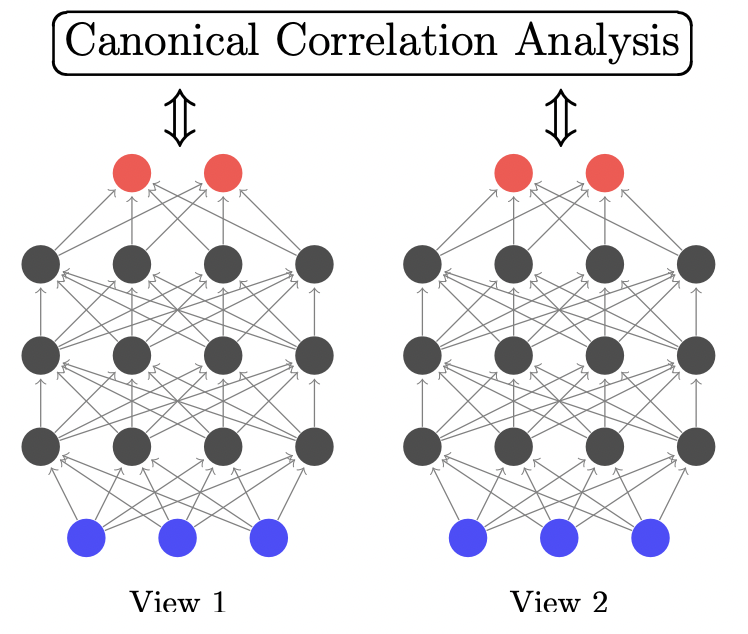
\includegraphics[scale=0.8]{figures/Theoretical_Background/DCCA.png}
    \caption{\en{The two parallel networks, along with the information path (arrows)}}
\end{figure}
\bigbreak

In the figure above, the two neural networks are shown, consisting of 5 layers, with the red layer being the output layer, meaning the vectors that are maximally correlated, and the blue layer being the input layer, meaning the original random vectors. 

If $θ_1$ is the vector of all parameters $(W_i^1, b_i^1)$ of the first network, for each layer i, and respectively $θ_2$ is the vector of all parameters $(W_i^2, b_i^2)$ of the second network for each layer, then the training goal is equivalent to finding the optimum parameters such that the correlation of the output of the networks $f_1(X_1; θ_1), f_2(X_2;θ_2)$ given two random vectors (views) $(X_1, X_2)$. 

That is described as follows:

\bigbreak
$(θ_1^\ast, θ_2^\ast)  = \operatorname{argmax}_{θ_1, θ_2} \{ corr(f_1(X_1; θ_1), f_2(X_2; θ_2))\}$
\bigbreak

Supposing that $H_1,H_2 \in \mathbb{R}^{o\times m}$ are the matrices that contain the respective outputs of the Neural Networks, for each of the  training samples. The target then becomes $corr(H_1, H_2)$. 

To train the networks, the computation of the gradient is needed, and its backpropagation in order to tune the networks parameters. The target is found using the same steps as the standard CCA, while the computation of the gradient, as well as its backpropagation is facilitated through singular value decomposition. 

The authors of the original paper employed full-batch optimization, meaning that before every single weight update step, the network scanned the full dataset. They also used the Limited Memory Broyden–Fletcher–Goldfarb–Shanno (L-BFGS) optimization method. In order to initialise the parameter optimization for the two networks, they utilised a denoising autoencoder for each layer of the networks. The network proposes uses a non-saturating nonlinearity activation function, in the form of:
If $g: \mathbb{R} \to \mathbb{R}$, and $g(x) = {\frac{x^3}{3}} + x$, then the function $s(x) = g^{-1}(x)$ is the activation function, maintaining a sigmoid shape, and unit slope at $x=0$. (\cite{43}, \cite{44})
}
    \subsection{\en{Multiple Correspondence Analysis}}
\en{Multiple Correspondence Analysis (MCA) is a data analysis technique used to analyse the structure of a number of dependent categorical variables in a dataset. It is an extension of simple Correspondence Analysis, and is similar to the well known method of Principal Component Analysis. \cite{45}


MCA is used when a dataset contains variables that are described by nominal values, such as "Male" and "Female", or "Red", "Green", "Blue", etc. The variables can also contain quantitative values, split into categories. MCA is performed on an indicator matrix - also called a Complete Disjunctive Table - or on a Burt table. It can also be viewed as the PCA method applied to the CDT. \cite{46}


Suppose there is a dataset containing only categorical variables, and its corresponding CDT, $X$. Let $K$ be the number of the nominal variables, and each nominal variable has $J_K$ levels and the sum of the $J_K$ is equal to $J$. There are $I$ observations. Then the table $X$ is actually the $I \times J$ indicator matrix. 

We indicate the sum of all entries to be $N$, and compute the probability matrix $Z = {
frac{X}{N}}$.
We also use the special vectors $r$, and $c$, which are the vector of the row totals of $Z$, and the vector of column totals of $Z$ respectively.

Then, if 
\bigbreak
$D_c = diag(c), D_r = diag(r)$, 
\bigbreak
we have the factor scores of the MCA are obtained from the following singular value decomposition: 

\bigbreak
$M = D_r ^{ -{\frac{1}{2}}} (Z - rc^\intercal) D_c ^{ - {\frac{1}{2}}} = P \Delta Q ^\intercal$,
\bigbreak  

where $\Delta$ is the diagonal matrix of the singular values, and the matrix of the eigenvalues is $\Lambda = \Delta^2$. 
MCA decomposes the matrix  into coordinates (or scores) of the factor space, which can be found as follows:
\bigbreak  
$F = D_r^{- {\frac{1}{2}}} P \Delta$, for the row coordinates and 
\bigbreak  
$G = D_c^{- {\frac{1}{2}}} Q \Delta$ for the column ones.
}

    \subsection{\en{Non-Negative Matrix Factorization}}
\en{Non-Negative Matrix Factorization (NMF) is a unsupervised, multivariate, analytic method for the approximate  factorization of a matrix $V$ into two matrices $W$,$H$ under the constraint that their elements are non-negative:
$V=WH$, such that $H\geq 0$ and $W\geq 0$. \cite{47}

The method was created by P. Paatero and U. Tapper, and further developed by D. Lee and H. Seung (\cite{48}, \cite{49}). It is used to reduce data dimensionality, perform clustering tasks and find underlying structures within the dataset. Because the resulting factorization contains non-negative elements, the method has the advantage of improved interpretability compared to other data dimensionality reduction methods, and has the ability to produce parts-based representation of the data, it has been applied in many different fields, such as machine learning, computer vision, signal processing, data mining, medical imaging etc. (\cite{50}, \cite{51}, \cite{52}, \cite{53})

Lee and Seung’s multiplicative update rule is the basis of the method’s computation of the $W$ and $H$ matrices, and has the characteristics of being iterative and element based. However there are other ways, and it can be supplemented with additional constraints or regularizations, leading to many extensions. 

One notable extension is that of Orthonormal Projective NMF (OPNMF), where the loading coefficients are estimated as the projection of the matrix  onto the estimated components $W$ ($H = W ^ \intercal V$), while maintaining orthonormality on the estimated components ($W^\intercal W = I$). As a result, all components participate in the reconstruction of all of the data samples, meaning that the overlap between the estimated components is significantly lower, having fewer parameters to be learned, while maintaining high sparsity. Additionally, this variant relies on the original update rule (and thus is computationally easier than the Projective NMF variant), and at the same time is able to generalize on unseen data without the need of retraining. \cite{50}
}
    \subsection{\en{Factor Analysis of Mixed Data}}
\en{Similar to MCA, Factor Analysis of Mixed Data (FAMD) is a data analysis technique used to analyse the structure of mixed data, meaning both continuous numerical as well as categorical data. It is also used to in order to reduce the number of dimensions of the dataset, and improve interpretability. It is based on the methods of MCA and PCA. \cite{55}

Suppose there is a dataset containing both quantitative (numerical) and qualitative (categorical) variables. Let $K_1$ be the quantitative variables, $Q$ the qualitative variables, and $K_q$ the categories of the $q^{th}$ variable. We can denote the overall number of categories of the qualitative variables as: 

\bigbreak
$K_2 = \sum_{q}^{} K_q$
\bigbreak

Let $K = K_1 + K_2 $ be the total number of quantitative variables and indicator variables.

We assume that individuals have the same weight, and the diagonal metric of the weights of the individuals is: 

\bigbreak
$D = {\frac{1}{I}}I_d$
\bigbreak

The quantitative variables are represented by a vector of length 1, and the qualitative ones by a cloud of datapoints $N_q$ of its centered indicators. FAMD aims to look for a direction  of $v$ that maximizes the inertia (measure of weighted spread of the points) of the $\mathbb{R}^{I}$ cloud. That goal is perfectly achieved by maximizing the following criterion:

\bigbreak
$\sum_{k\epsilon K_1}^{} r^2(k,v) + \sum_{q\epsilon Q}^{} \eta^2(q,v)$  , where
\bigbreak
$\eta^2(q,v)$ is the squared correlation ratio between $q$ and $v$, and $ r^2(k,v)$  is the squared projection coordinate of variable $k$ on $v$. \cite{56}

FAMD's number of resulting components can range from $1$ to $min(K_1, Q)$, where $K_1$ is the number of the quantitative variables and $Q$ is the number of the categorical ones.
}
    \subsection{\en{Support Vector Machines}}
\en{Support Vector Machines are a family of models that are used for classification and regression analysis. The model was initially introduced by C. Cortes and V. Vapnik and has enjoyed considerable popularity since its creation, being one of the most widely used Machine Learning Techniques. They have been applied to many scientific fields, such as pattern recognition, image classification, biomedical research, petroleum exploration, etc.(\cite{57}, \cite{58}, \cite{59})  

The goal of an SVM is to choose a hyperplane (e.g. a straight line in two-dimensional space, a plane in three-dimensional) that best separates a dataset consisting of labeled samples that belong to one of two classes. The method that SVMs rely on to achieve this goal is choosing two parallel hyperplanes that separate the two classes such that the distance between them (the margin) is maximal. The data points on the margin maximizing hyperplanes (supporting vectors)  define the decision surface for the classification, as shown below: \cite{60}

\bigbreak
\begin{figure}[h!]
    \centering
    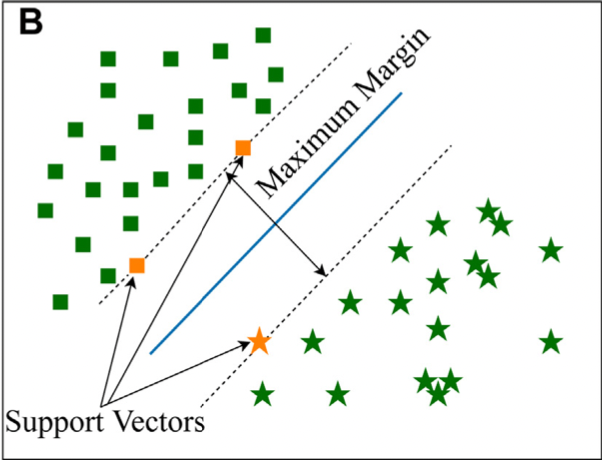
\includegraphics[width=0.5\textwidth]{figures/Theoretical_Background/SVM.png}
    \caption{\en{Support Vectors are shown in orange, the decision boundary in blue, the datapoints in green (squares for one class, stars for the other), and the dash lines are the margin maximizing hyperplanes. \cite{60}}}
\end{figure}
\bigbreak

SVMs can be used for multi-class classification as well, through a one-vs-one scheme or one-vs-rest approach, where decision boundaries are calculated between respective classes or a class and the rest of the dataset in each case, respectively. \cite{61}

SVMs enjoy a variety of advantages, such as efficiency in both low and high dimensional spaces, memory efficiency, and being able to produce results in cases where the number of samples is less than the number of dimensions. \cite{62}

However, one major drawback of SVMs is that the standard model does not work on datasets that are not linearly separable; that is one hyperplane cannot correctly divide the classes. To get around that, SVMs use kernels. Thus, the dataset is first non-linearly mapped through a kernel in a higher dimension space where the data is linearly separable, and then the original SVM algorithm is performed. In this approach, one can use the kernel trick to compute the transformations through the kernel function for the whole dataset. \cite{60}

SMVs suffer from over-fitting issues, as well as being sensitive to parameter selection/tuning, such as the kernel function and regularization term choice, especially if the number of parameters is much greater than the number of available samples. Additionally, SVMs are not scale invariant, so scaling the dataset is highly recommended. (\cite{62}, \cite{63}
}
    \subsection{\en{Ensemble Learning}}
\en{Ensemble learning is a technique of combining a multitude of models to enhance the performance of the task, such as classification problems, regression or approximation tasks etc. This is achieved by applying the (perhaps different) models to the data available (or a subset thereof) and combine their outputs, in order to make a better attempt at solving the problem. \cite{64}

An ensemble is created by combining either different models, or models with different parameter initializations and configurations. Such models can be relatively simple, such as decision trees, naive bayes classifiers, or SVMs, or more complicated, such as multi layer perceptrons, or even other ensembles altogether. A key aspect of the base model selection is to create enough diversity of opinions, that is differentiation between the models themselves. \cite{65}

The ensemble learning technique relies on two concepts: the way the dataset is used to train the base models (how the data is introduced to the models) and the way that the outcome of each base model is considered towards the combined outcome. 

The method that is employed for training the base models can be as simple as dividing the dataset by the number of models and feeding each subset to each model, or as strategically complex as to involve feature selection along with data augmentation during the phase of training the base models. Another approach might be introducing different views of the dataset to different base models. \cite{65}

Respectively, the method employed for combining the outcomes of the base models can be as simple as simple majority voting (for example the most voted class in a classification problem) or algebraic combiners, or more sophisticated and tailored to a specific problem strategies. 

The idea behind ensemble learning is to enhance the decision taken with group knowledge; that is to reduce the likelihood of an unfortunate selection. While that is not guaranteed, there is empirical evidence that ensemble models achieve in general better performance than that of single models, and in some case better than that of the average of their base models. \cite{65} 



Another motive for employing ensemble methods is their ability to perform fairly well both in big data tasks and when there isn't adequate data for the successful training of a single model. The big data case is handled with dividing the dataset into many subsets, and training each model on a single subset, thus making the training phase much easier. On the other hand, with a strategy such as bootstrapping, different base models can be trained on different combination of samples of data, taken from the initial dataset, with replacement, and treated as if they were independently drawn. (\cite{65}, \cite{66})
\bigbreak
\begin{figure}[H]
    \centering
    \includegraphics[width=0.7\textwidth]{figures/Theoretical_Background/EnsembleLearning.jpg}
    \caption{\en{Combining classifiers with different decision boundaries reduce error. \cite{68}}}
\end{figure}
\bigbreak
One method of ensemble learning applied to the problem of classification is that of Bagging, or Bootstrap Aggregating, where the base models are trained on drawn samples from the initial dataset, with replacement, and the base models are classifiers of the same type. The individual classifiers' outcomes are combined in a simple majority voting strategy to determine the overall outcome of the ensemble. Another notable example is that of Adaboost, a version of the boosting ensemble, adapted for the problem of multiclass classification. As previously, bootstrapped training data samples are drawn from an initially uniform but  continuously evolving distribution, ensuring that samples that were previously mislabeled are seen more often, and therefore training the base classifiers to the most difficult instances. The base classifiers are combined in a weighted majority voting manner.  (\cite{65}, \cite{67})
}
    %%%%%%% Methodology %%%%%%% 
    % Data Pipeline Overview %
    \chapter{\tl{Methodology}}
\section{\tl{Data Pipeline Overview}}
\en{The data of this thesis were obtained from the Alzheimer’s Disease Neuroimaging Initiative (ADNI) database, a global research study that focuses on understanding better how to prevent or delay the disease, as well as supporting the investigation on methods of treatment. The study collects imaging, genetic, clinical, biospecimen data from people with MCI, Alzheimer’s, as well as from people that are Cognitively Normal (CN). The data was collected in 4 phases, ADNI1, ADNI2, ADNIGO and ADNI3. This study uses data from all three phases, however only uses the genetic and imaging views of the dataset. For more information on the dataset, please visit  \href{https://adni.loni.usc.edu/methods/documents/}  . \cite{69}

The imaging data is in the form of 145 ROI values, acquired from scanners either 1.5T or 3T, using T1-weighted sequences, depending on the phase. The images collected by the scanners have been filtered through Quality Control, and have been preprocessed through intensity normalization and gradient un-warping. In order to acquire the ROI intensity values, the method of MUlti-atlas region Segmentation utilizing Ensembles (MUSE) was used creating the regions of interest. ROIs values’ magnitude is analogous to the regional volume of brain tissue, depending on tissue type. The Regions that these values correspond to can be found in the appendix. (\cite{70}, \cite{71}) 

As for the genetic data, each participant has values for 54 susceptibility loci, in the form of SNPs, that have been identified by AD genetics studies. These values have been filtered through QC, and as previously mentioned are int the form of number of alleles (0,1,2) for each SNP. (\cite{72}, \cite{73}, \cite{74}, \cite{75})
\begin{figure}
  \centering
  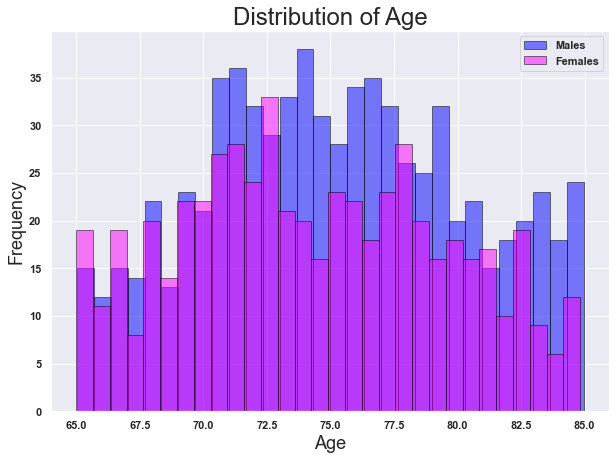
\includegraphics[width=.7\linewidth]{figures/Methodology/sex_histogram.png}
  \caption{\en{Distribution of age for participants}}
\end{figure}%
\begin{figure}
  \centering
  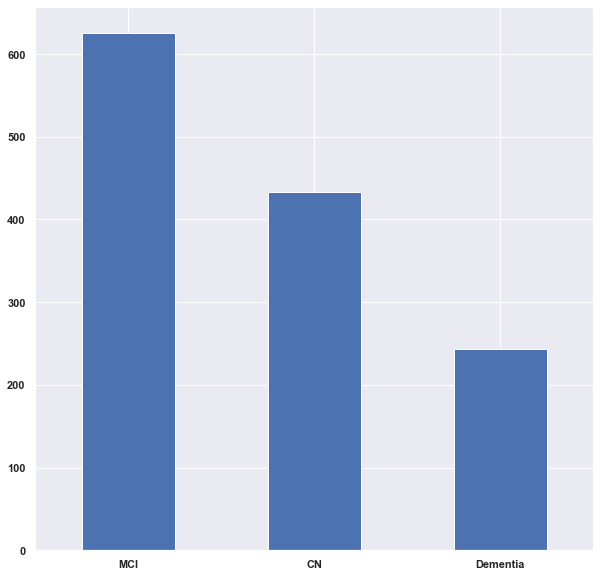
\includegraphics[width=.7\linewidth]{figures/Methodology/classes_bars.png}
  \caption{\en{Distribution of classes for participants}}
\end{figure}
\bigbreak
The dataset has 1302 participants, (56.91\% male), with mean age 75.20 y.o. for males and 74.36 y.o. for females. The dataset now has 433 CN participants (33.25\%), 626 MCI patients (48.07\%) and 243 AD patients (18.66\%). Following that, Linear Regression was performed to remove any unwanted age, sex, or brain size related effect. The regressor was fitted on the CN group, and the transformation was applied to the entire sample. Subsequently, the data was transformed through experimentation, and the output of the method was stored, in order to be compared with the raw data. Afterwards, data analysis techniques were applied, such as OPNMF to the imaging data, or MCA to the genetic data, or FAMD to the whole dataset. These methods were applied both to the original data, as well as the output of the DCCA method, in order to be compared later. The result of each one of those techniques was then saved for later tasks. Finally, each one of the results of combinations of the methods was fed to SVM as well as ensemble classifiers. 
\begin{figure}[H]
    \centering
    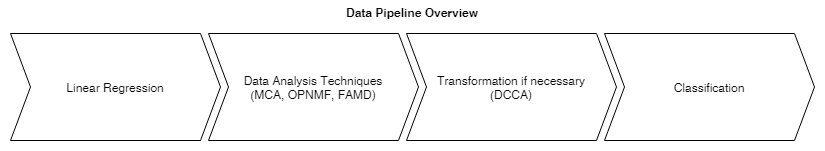
\includegraphics[width=\textwidth]{figures/Methodology/Data_Pipeline_Overview.png}
    \caption{\en{Data Pipeline Overview}}
\end{figure}
\begin{figure}[H]
    \centering
    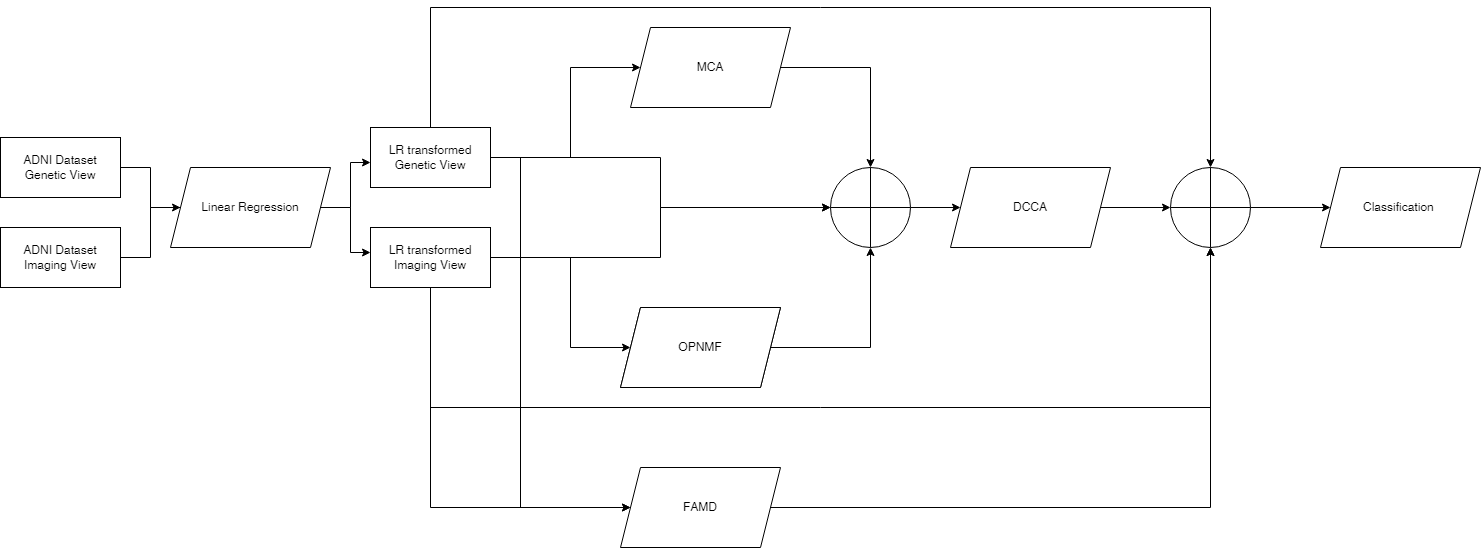
\includegraphics[width=\textwidth]{figures/Methodology/Data_Pipeline_Diagram_1.png}
    \caption{\en{Data Pipeline Diagram}}
\end{figure}
\bigbreak
}
    % Linear Regression %
    \section{\tl{Linear Regression}}
\en{Linear Regression is a statistical method that aims to learn the relationship between dependent and independent variables. In our case, the goal is to study the shrinkage effect that AD and MCI have on brain size, and therefore to study it properly we need to isolate that effect. In order to do that, any effects that age, sex and different cranium sizes have, must be removed. Finding out the pattern between the brain size, which is the 145 ROI values, and the age the person has, as well as his/her gender and cranium size, is necessary if we want to remove it.

LR learns the trend between the independent variables (age, gender, cranium size) and the dependent variable (ROI volume), so calculating the difference from the computed trend values and the real values is called the residual values. We use those residual values as a means to recognize how intense the effect of the disease on the participant’s brain size is, since the other independent variables’ effects have been subtracted, meaning that if there was no effect, the trend between age, gender and cranium size would accurately predict the brain size and there would be no error. 

The model is trained on CN participants only, however all participants brain sizes are predicted using the trend line learned, to find out the difference between the real values and the predicted ones. We only keep the residual values, as they signify the difference from the trend line, which is equivalent to the intensity of the disease’s effect. 

The trend lines can be observed in the below figure for the ROI MUSE\_Volume\_48 which is translated to the left hippocampus area. It is clear that while the CN (green) population is centered around the x axis, meaning the brain size values are well predicted, the MCI population (blue) is lower than predicted, and the AD population (red) is much lower. This is expected, as the real brain size values are lower, since MCI and AD both cause a shrinkage of the brain.
\bigbreak
\begin{figure}[H]
    \centering
    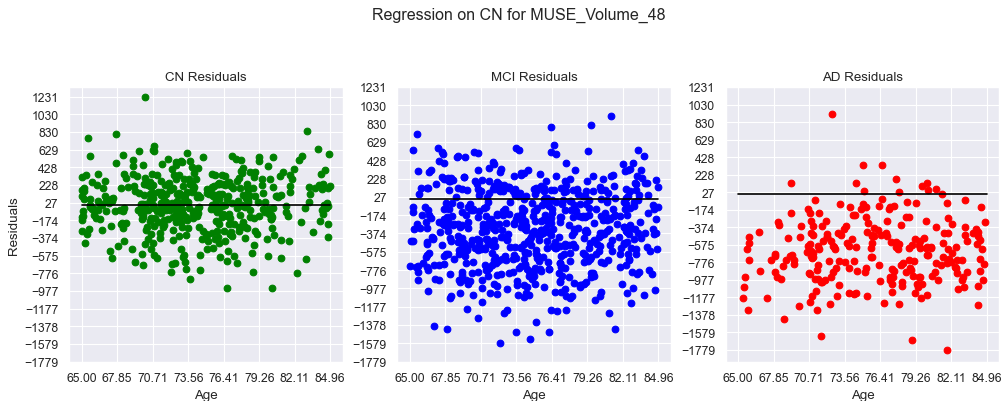
\includegraphics[width=\textwidth]{figures/Methodology/Linear_Regression.png}
    \caption{\en{Linear Regression on CN for MUSE\_Volume\_48}}
\end{figure}
\bigbreak

}
    % DCCA model training %
    \section{\tl{DCCA model training}} \label{DCCA methodology}
\en{In addition to the previously mentioned techniques, DCCA was used in order to transform the two uncorrelated, different views into two that are more linearly correlated. The choice of hyperparameters, the methods and class functions, as well as the parameter optimization was subject to our experimentation. 

As stated before, the DCCA model relies on two parallel networks, each taking as input a view of the dataset, and producing the output that are the views but nonlinearly transformed in order to use as subject for classification. 

The dataset for the model optimization was split into three sets, the training, validation and the test set, with the last one being kept hidden from the model during the training phase, in order to ensure an accurate prediction on unseen data. The split between the sets was 75\% for the training set, 15\% for the validation set, and 10\% for the test set, split randomly. This was done in order to ensure that the model had enough training samples, as well as validation samples to achieve good accuracy scores without overfitting, and enough test scores as to not skew the results. 

The hyperparameters include the number of hidden layers as well as hidden layer size, output layer size, the regularization parameter, the learning rate, as well as the batch size. These hyperparameters were chosen after extensive testing with each one, with the best values stored and used for training. The epoch number was kept at 100 epochs along all experimentation, which was enough for all cases for the validation accuracy score to stabilize. 

We experimented with 3 or 4 hidden layers, as it became apparent that due to the complexity of the problem, a big enough network was needed for both views. The original paper used the same architecture for both of the networks, a logic we followed in our study as well. The size of the hidden layers ranged from 256 neurons to 1024 neurons per layer, with all hidden layers having the same number of neurons. As for the output layer size, we experimented with sizes of [10,50,100,150]. One attempt was made with output layer size of 300 in order to observe the effect of large output layer size in the correlation metric, however the computation was extremely time-consuming. Furthermore, the learning rate ranged from $10^{-4}$ to $10^{-2}$, and the regularization parameter being in the range of $10^{-4}$ to $10^{-2}$. The batch size that we used was either 500 samples or 1000 samples. 

The activation function was kept the same as the original paper, which was a sigmoid function, and the error metric was the error metric as defined from the paper, a version of CCA using a derivative-free optimization method. The optimizer function of the paper was the L-BFGS second-order optimization method, however due to it being more difficult to compute, the optimizer RMSProp was used, with similar results. The original paper initialized the neural network using a denoising autoencoder, but this was out of the scope of this study.  \cite{76}

The DCCA implementation we used was made with python by Z.Wu. The method is implemented with pytorch, which supports for multi-GPU training, however this study employed only CPU training.  (\cite{77}, \cite{78})
}
    % Data Analysis Techniques %
    \section{\tl{Data Analysis Techniques}}
\en{In our experimentation with the dataset, it was noticed early that the nature of the different types of views of the dataset was an obstacle to the methods and the goals we wanted to achieve. We hypothesized that the difficulty to achieve better classification scores stemmed from the fact that the two views of data were different not only in type (numerical vs categorical), but in the difference of the dimensions as well, making the algorithms employed inefficient and/or not well suited for the task.

To remedy this situation, we experimented with data analysis techniques. Initially we tried OPNMF, to reduce the number of imaging dimensions, to more closely match the number of genetic dimensions. Then, we tried using MCA to transform the genetic data from categorical to numerical, and finally we tried creating a combining transformation of the two views using FAMD, as a benchmark for the other methods. All possible combinations of the methods were tested, in order to find the best possible mix.

A data analysis technique that this study explores is that of Orthonormal Projective Non-Negative Matrix Factorization. This method is used to dimensionally reduce a dataset, while still maintaining interpretability, due to the non-negative nature of the matrix decomposition. For this dataset, we applied OPNMF to the RAVENS maps of the imaging data, because it has been observed to achieve better results than the MUSE ROIs, while reducing the dataset dimensions. In this work, the imaging data was reduced into 30 components. \cite{79}

The number of the resulting components was chosen in a way that was close to the number of the number of dimensions of the genetic data, close to the (later referenced) number of MCA components, while not too small in order to retain most of the information and minimize approximation error, and not too big in order for the method to have any use. It is worth noting that the OPNMF method rescales the data, a much needed action, since different ROIs have orders of magnitude different intensities, a feature that the SVM classifiers benefit from.

Another data analysis technique that is used in this study is Multiple Correspondence Analysis, which, as previously mentioned, analyses the structure of a number of dependent categorical variables, and performs dimensionality reduction if necessary. For this dataset, we applied MCA to the genetic data, in order to dimensionally reduce the 54 SNPs into 10 components. This had the added benefit of transforming the categorical data into numerical, which we hypothesized would greatly enhance the outcome of the classification.

The method was performed using mca, a package for python which is intended to be used along with pandas. \cite{80}

The third and final technique we explored is Factor Analysis of Mixed Data, which combines multiple views of the dataset, to create a transformation along with a dimensionality reduction. 

The number of the resulting components was chosen based on the fitting time, however it was quickly observed that above 12 components, the time needed for computing the resulting components was more than substantial, making the process of optimizing quite lengthy and not feasible. 

The method was based on the implementation of the python package prince, an open-source package developed by Max Halford. \cite{81} 
}
    % Classification% 
    \section{\tl{Classification}}
\en{The task we tried to enhance the models for was the one of classification. To solve that, we chose the SVM family of models, and optimized it through parameter grid search, which is exhaustive search of all the different parameter combinations.

As mentioned previously, SVMs can have different kernels, in order to accommodate for non-linear datasets. We experimented with linear, polynomial, and radial basis function kernels, which are among the most commonly used. For each kernel, its specific parameters were optimized through grid search, and the results were evaluated on their ability to generalize through cross validation. 

For all of the different cases, we used the python library Scikit-Learn, and specifically the sklearn.svm module. \cite{82}

In particular, for the linear kernel we experimented with L2 normalization penalty, [0.00001, 0.0001, 0.001, 0.01, 0.1, 1, 10] C (regularization parameter) values, and one-vs-rest multi class classification strategy. As for the polynomial kernel, we experimented with polynomial degrees of [2,3,4,5], independent term values of [0.00001, 0.0001, 0.001, 0.01, 0.1, 1, 10], C values of [0.00001, 0.0001, 0.001, 0.01, 0.1, 1, 10], and finally kernel coefficient values (g values) of [0.0001, 0.001, 0.01, 0.1, 1]. Finally, as for the radial basis function kernels, we experimented with C values of [0.00001, 0.0001, 0.001, 0.01, 0.1, 1, 10], and kernel coefficient values of [0.0001, 0.001, 0.01, 0.1, 1]. 

Each kernel was given 1000 iterations in order to converge, and the cross validation was done with 5 folds. The data was split into train and test splits, with respective sizes of 80\% and 20\% of the initial dataset, without shuffling, as the data was already ordered randomly. All of the combinations were run on all of the potential different combinations on views of every data analysis techniques (imaging + genetic views, only imaging, only genetic). 

Furthermore, in addition to the simple method of the SVM models, we attempted to use the method of ensemble learning to further enhance the classification outcome. For that reason, we experimented with the methods of Bagging (Bootstrap Aggregating) and Adaboost. For both of those methods, we experimented with the base classifier being a decision tree or a linear SVM. 

For all of the different combinations, we used the python library Scikit-Learn, and specifically the sklearn.ensemble module.

The parameter tuning for both of those models as well as their base classifiers was done with grid search along with cross validation, using 5 folds. Specifically, for the Bagging classifier ensemble model, the parameters that we experimented with were the number of estimators, with values of [5,10,15], the maximum samples of the dataset that an estimator could train on, with values of [60\%,80\%,100\%]. As for the Adaboost ensemble classifier model, the parameters we experimented with were again the number of estimators, with those being [5,10,15,50], and SAMME and SAMME.R for the boosting algorithm. The learning rate for this model was kept at 1.0.

For the decision tree base classifier, the parameters we experimented with were the estimator criterion, with it being either gini Impurity or entropy, along with the max depth, with its values being [1,2,5]. Finally, for the linear SVM base classifier, we experimented with the C parameter, with its values being [0.00001, 0.0001, 0.001, 0.01, 0.1, 1, 10].

Before the classification task, if needed, balancing and scaling was applied. Balancing the dataset was done through random undersampling, while scaling was performed utilizing scikit-learn's preprocessing module, and more specifically the StandardScaler function. This function standardizes features by removing the mean and scaling to unit variance.

The metrics we chose for the classification task were those of accuracy, balanced accuracy, and F1 score. The implementation of the metrics that was used was again from Scikit-Learn. As for accuracy, it is the ratio of: 

\bigbreak
$Accuracy \; = \;{{\frac{True\;\; Positive\;\; +\;\;True\;\; Negative}{True\;\; Positive\;\; + \;\;False \;\;Positive\;\; + \;\;True\;\; Negative\;\; + \;\;False\;\; Negative}}}$
\bigbreak

As for the balanced accuracy, it is the ratio of:

\bigbreak
$Balanced \;\;Accuracy \; =Avg({\frac{True\;\;Positive} {True \;\;Positive \;\;+\;\; False \;\;Negative} }+ {\frac{True \;\;Negative}{True \;\; Negative \;\;+\;\;False \;\;Positive}})$
\bigbreak

And as for the F1 score, it is the ratio of:
\bigbreak
$F1 \;\; Score = {\frac{True\;\; Positive\;\;}{ True\;\; Positive\;\; + \;\;{\frac{1}{2}}( False \;\;Positive\;\; + \;\;False\;\; Negative)}}$
\bigbreak
}
    %%%%%%% Optimizations %%%%%%% 
    \chapter{\tl{DCCA Optimizations}}
\en{Before the classification, we must optimize the DCCA network parameters, and find the ideal values and combinations. We do that for the different cases of the views. 

First of all, we train the DCCA networks on the raw data, meaning the 145 ROI values for the imaging view, and the 54 SNPs for the genetic view. After that, we take the MCA-transformed genetic data (10 genetic components), and pair them with the original imaging data, meaning the 145 ROI values. Finally, we experiment with the opposite combination, which is the OPNMF-transformed imaging data (30 imaging components) and pair them with the original genetic data, meaning the 54 SNPs. 

As mentioned in the previous chapter, the parameter combinations we explored affect the number and sizes of the hidden layers, the size of the output layer of the network, the learning rate, the regularization parameter and the batch size. The following results are after exhaustive search of the different parameter combinations. 

The metric we optimized for is the correlation between the two views, after being transformed by their respective DCCA network. Essentially we pass the data through their own trained network, transforming them and measuring how linearly correlated they have become. The total number of parameter combinations for each different case of the views is 288.

For each parameter, we plotted for the different values the correlation achieved by the worst combination of the parameter’s value with all the other possible parameters values, the average correlation, as well as the best correlation. Since the implementation of the DCCA network employed the correlation as a Loss function (assigned with a negative signum, in order to be able to be minimized), we used that as the metric directly. 

\section{\tl{Original data: 145 ROI (Imaging) + 54 SNPs (Genetic)}}

\begin{figure}[H]
    \centering
    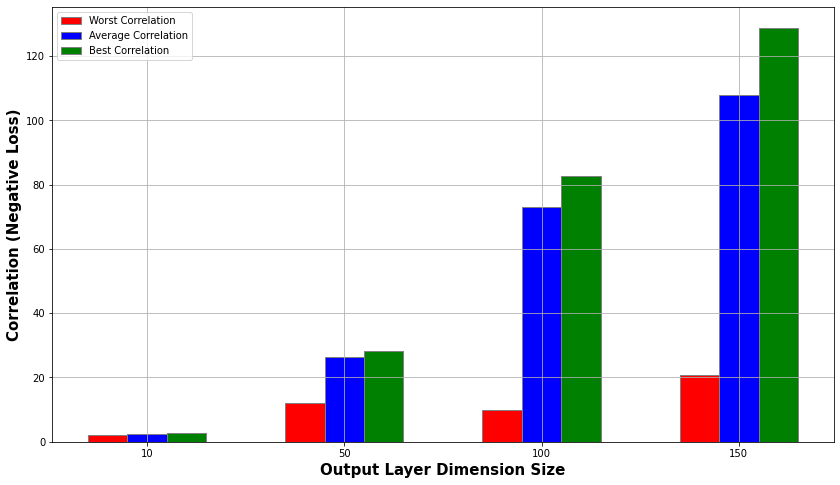
\includegraphics[width=\textwidth]{figures/DCCA_optimizations/Raw_Outdim.png}
    \caption{\en{Output Layer Dimension size vs Achieved Correlation}}
\end{figure}
\begin{figure}[H]
    \centering
    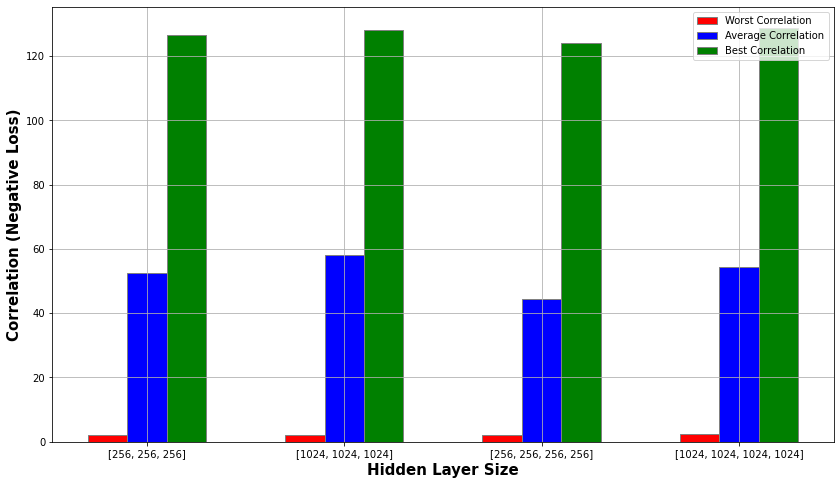
\includegraphics[width=\textwidth]{figures/DCCA_optimizations/Raw_Hidden.png}
    \caption{\en{Hidden Layer size vs Achieved Correlation}}
\end{figure}
\begin{figure}[H]
    \centering
    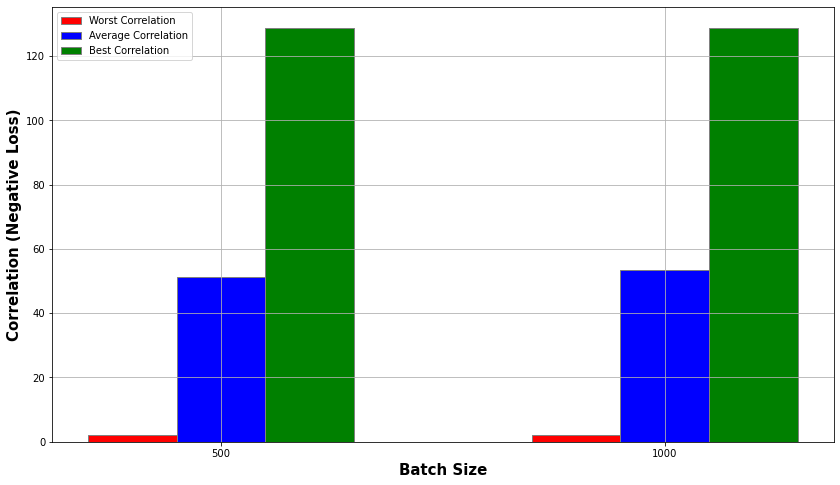
\includegraphics[width=\textwidth]{figures/DCCA_optimizations/Raw_Batch.png}
    \caption{\en{Batch size vs Achieved Correlation}}
\end{figure}
\begin{figure}[H]
    \centering
    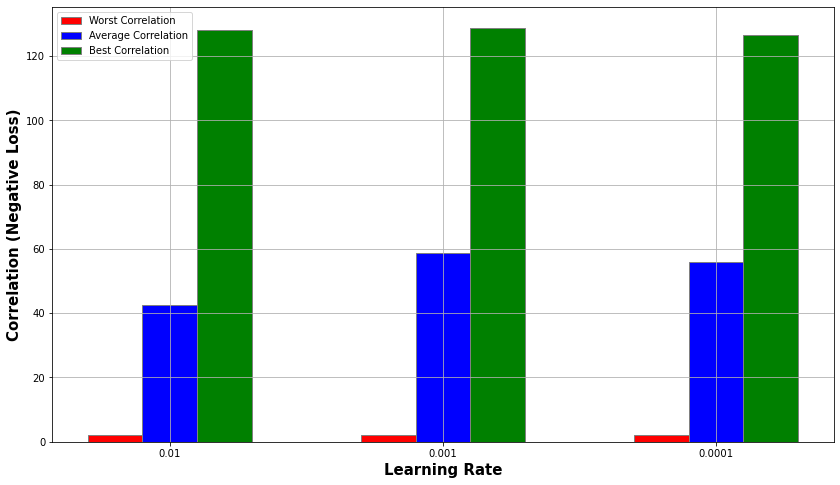
\includegraphics[width=\textwidth]{figures/DCCA_optimizations/Raw_Learning.png}
    \caption{\en{Learning Rate vs Achieved Correlation}}
\end{figure}
\begin{figure}[H]
    \centering
    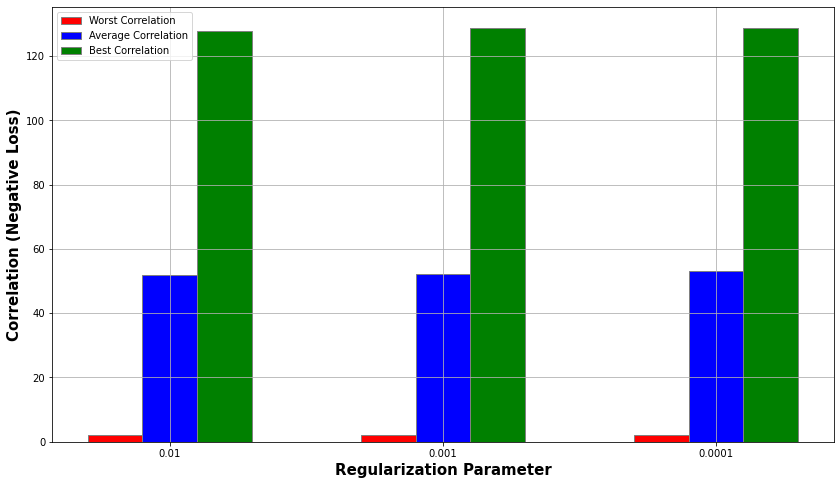
\includegraphics[width=\textwidth]{figures/DCCA_optimizations/Raw_Regularization.png}
    \caption{\en{Regularization Parameter vs Achieved Correlation}}
\end{figure}


Based on the above figures, it is clear that the more nodes the output layer has, the better the correlation of the transformed data is, not only on the best case, but on average as well as on the worst case. 

Furthermore, it is clear that the hidden layer size and number have little effect on the output correlation, since not only the best, but also the average and the worst cases, the correlation numbers seem to be the same. It can be noted that more hidden layers and more nodes per hidden layer do seem to be achieving better results, but the difference is minor.  

As for the batch size parameters, in our experiments the results stay basically identical; the only change being noticed in terms of training time, since the lower the batch size, the more time the model takes per epoch to run through the dataset, hence more training time for the same number of epochs. 

The same effect can be noticed with the Learning Rate, since the best case is more or less achieving the same results, however here we can observe that the average case benefits from a medium Learning Rate value of 0.001. 

Finally, the Regularization parameter follows the same logic, with its changing not making a substantial difference, and on all accounts the results being identical. 

To summarize the parameters' effects, we can create the following table:

\begin{figure}[H]
    \centering
    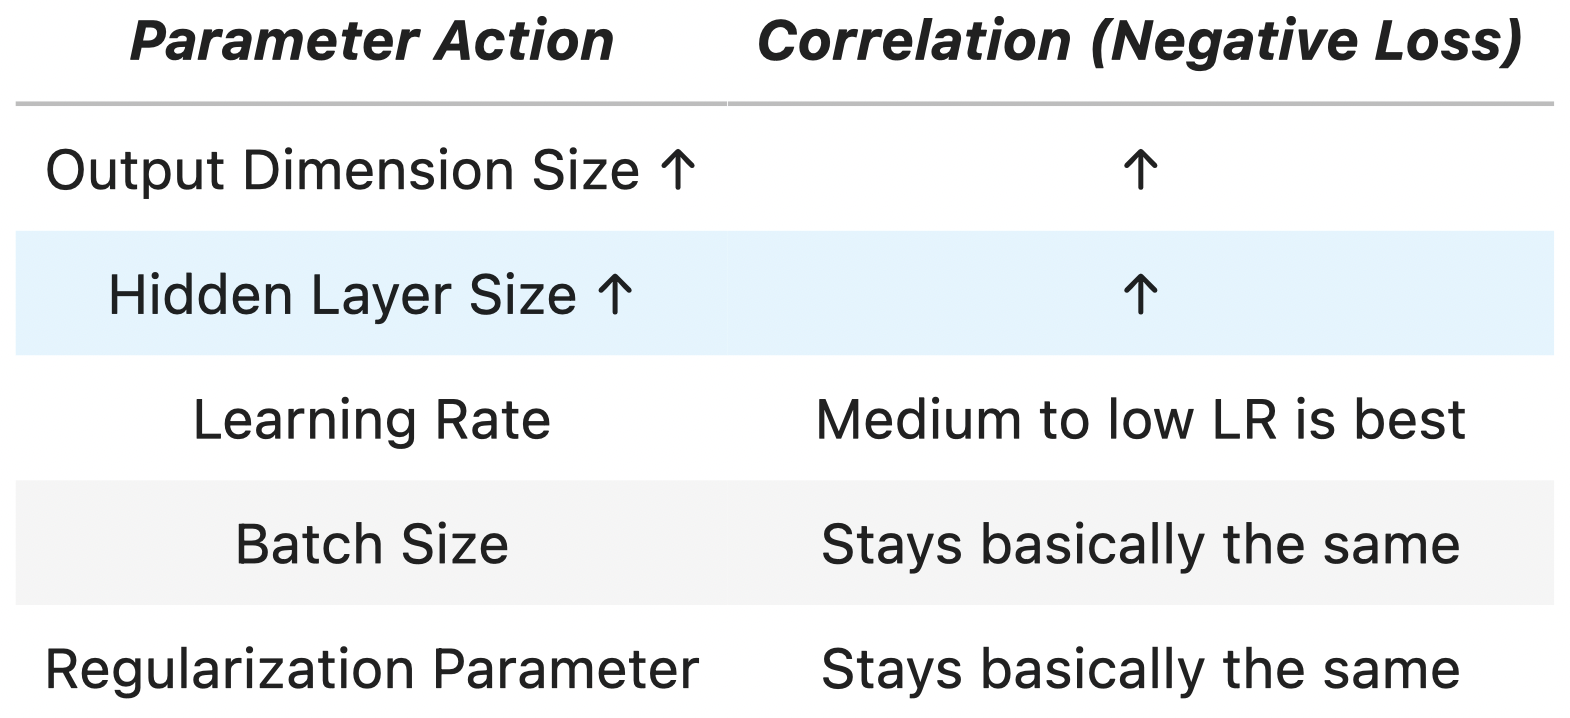
\includegraphics[width=0.7\textwidth]{figures/DCCA_optimizations/Raw_Conclusions.png}
    \caption{\en{Learned Conclusions from DCCA optimizations on 145 ROI (Imaging) and 54 SNPs (Genetic)}}
\end{figure}

\section{\tl{Transformed Genetic data: 145 ROI (Imaging) + 10 MCA components (Genetic)}}
\begin{figure}[H]
    \centering
    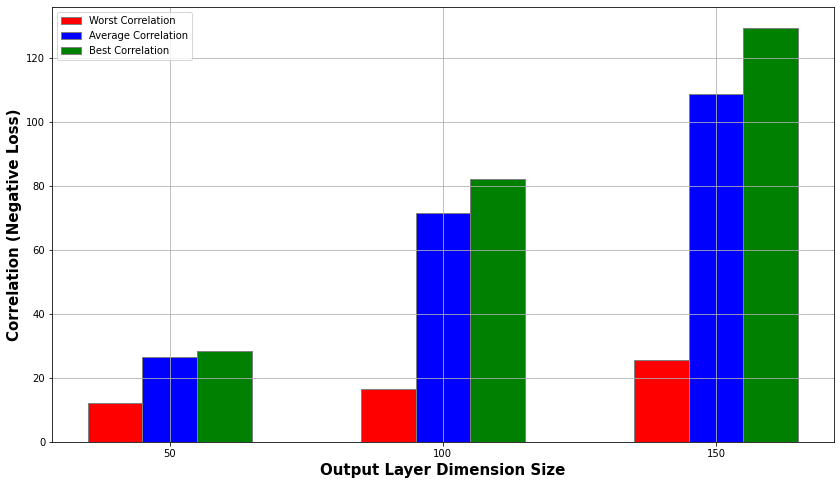
\includegraphics[width=\textwidth]{figures/DCCA_optimizations/MCA_Outdim.png}
    \caption{\en{Output Layer Dimension size vs Achieved Correlation}}
\end{figure}
\begin{figure}[H]
    \centering
    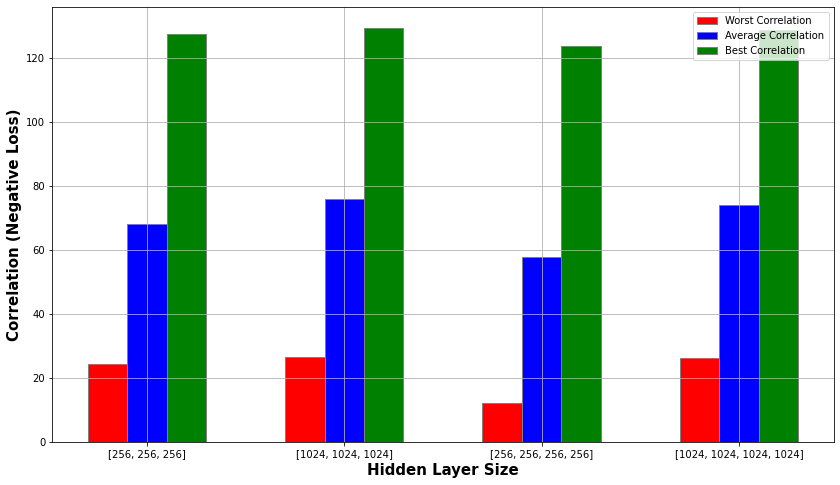
\includegraphics[width=\textwidth]{figures/DCCA_optimizations/MCA_Hidden.png}
    \caption{\en{Hidden Layer size vs Achieved Correlation}}
\end{figure}
\begin{figure}[H]
    \centering
    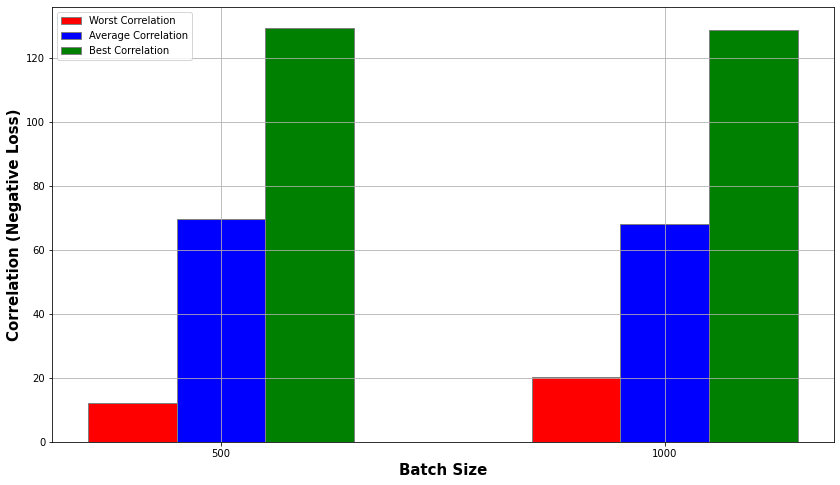
\includegraphics[width=\textwidth]{figures/DCCA_optimizations/MCA_Batch.png}
    \caption{\en{Batch size vs Achieved Correlation}}
\end{figure}
\begin{figure}[H]
    \centering
    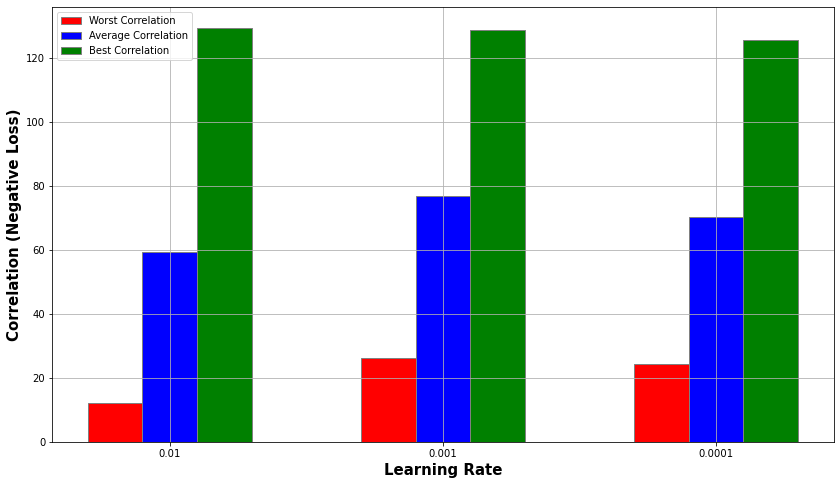
\includegraphics[width=\textwidth]{figures/DCCA_optimizations/MCA_Learning.png}
    \caption{\en{Learning Rate vs Achieved Correlation}}
\end{figure}
\begin{figure}[H]
    \centering
    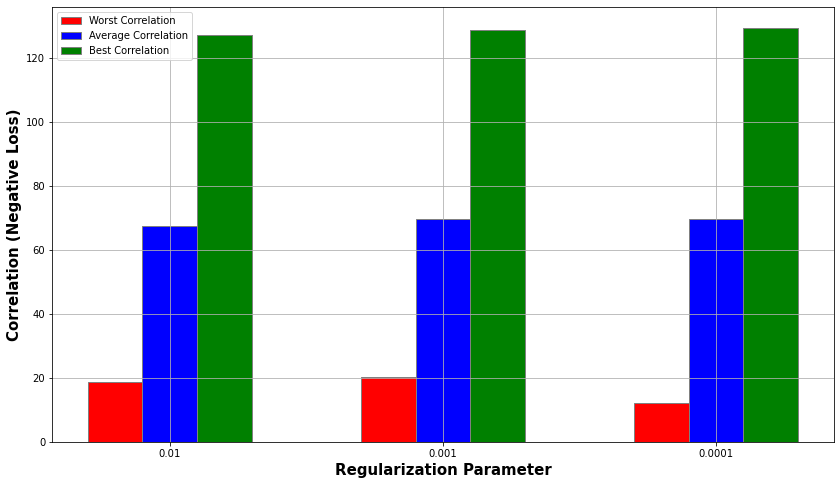
\includegraphics[width=\textwidth]{figures/DCCA_optimizations/MCA_Regularization.png}
    \caption{\en{Regularization Parameter vs Achieved Correlation}}
\end{figure}

As before, we notice the same patterns. Increasing the output layer size results in an increase in output correlation, hidden layer size and number of hidden layers seems to make a small difference, and for the rest of the parameters the effect seems to be negligible. We can sum up the parameter behaviour in the following table:
\begin{figure}[H]
    \centering
    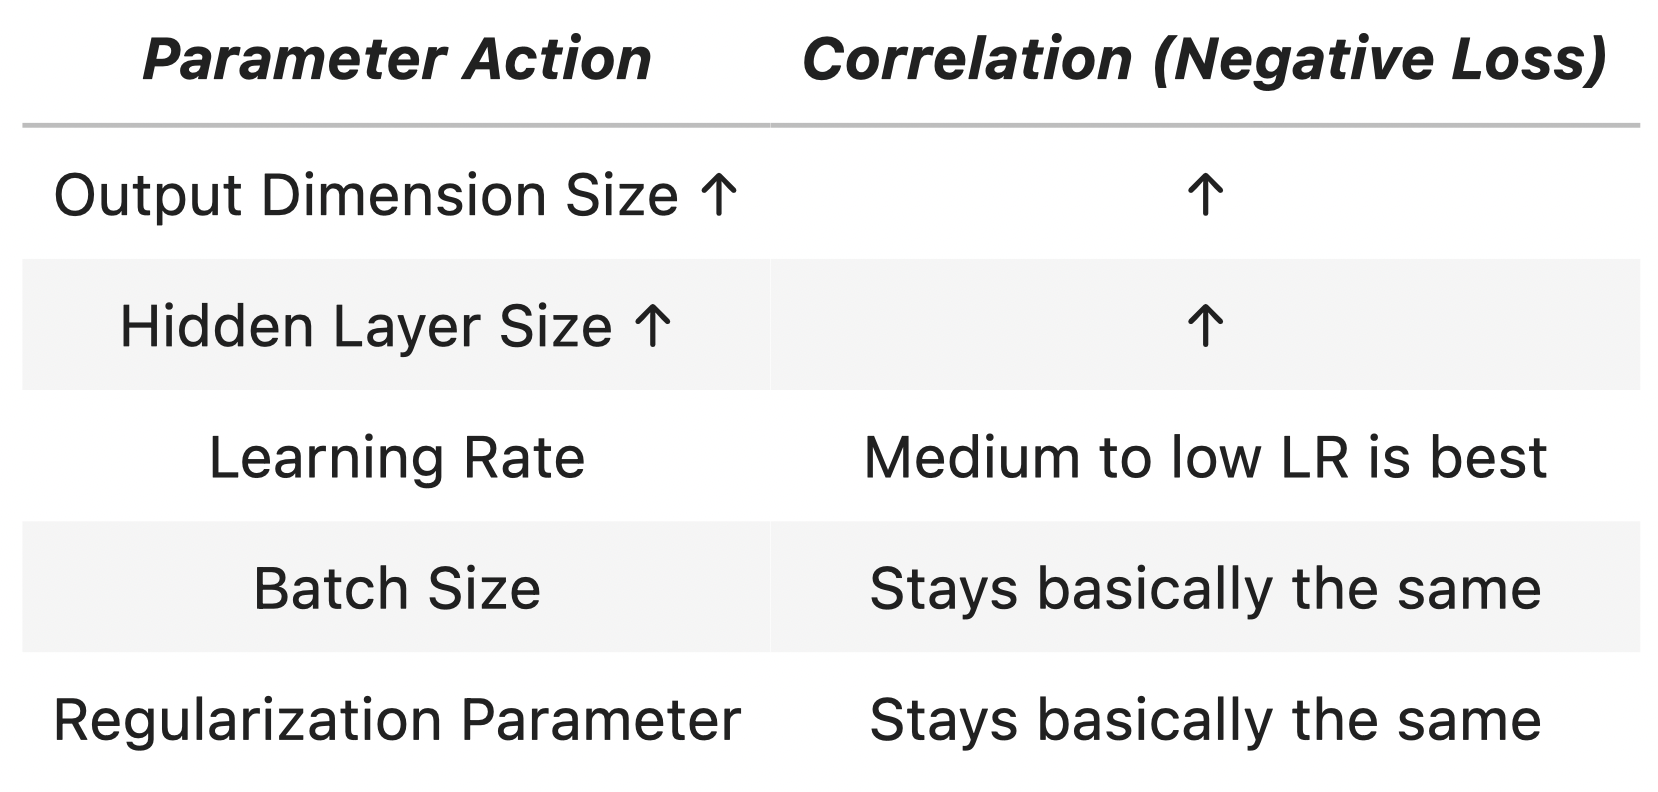
\includegraphics[width=0.7\textwidth]{figures/DCCA_optimizations/MCA_Conclusions.png}
    \caption{\en{Learned Conclusions from DCCA optimizations on 145 ROI (Imaging) and 10 MCA Genetic components}}
\end{figure}


\section{\tl{Transformed Imaging data: 30 OPNMF components (Imaging) + 54 SNPs (Genetic)}}

\begin{figure}[H]
    \centering
    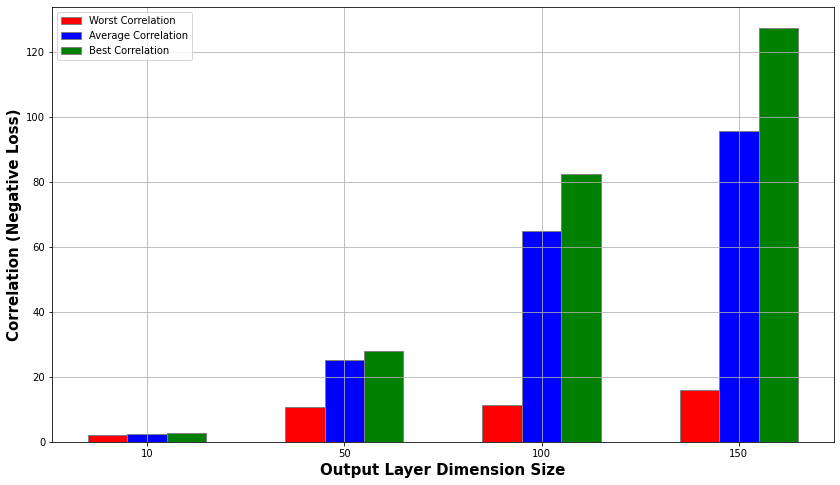
\includegraphics[width=\textwidth]{figures/DCCA_optimizations/NMF_Outdim.png}
    \caption{\en{Output Layer Dimension size vs Achieved Correlation}}
\end{figure}
\begin{figure}[H]
    \centering
    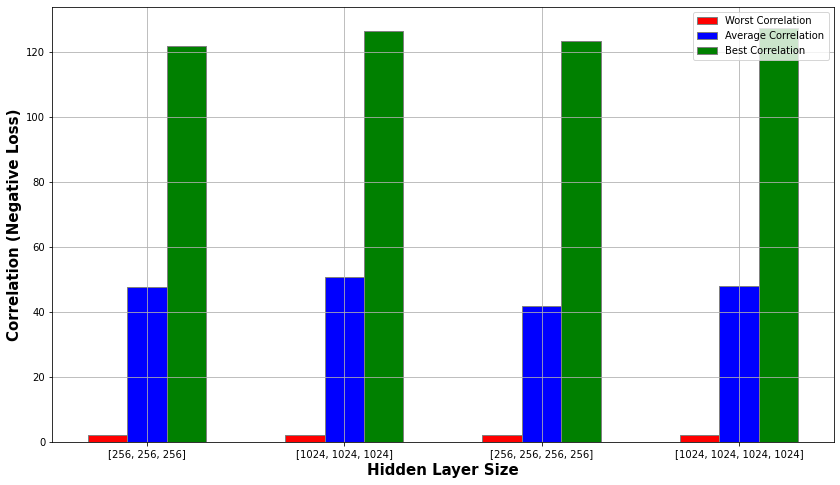
\includegraphics[width=\textwidth]{figures/DCCA_optimizations/NMF_Hidden.png}
    \caption{\en{Hidden Layer size vs Achieved Correlation}}
\end{figure}
\begin{figure}[H]
    \centering
    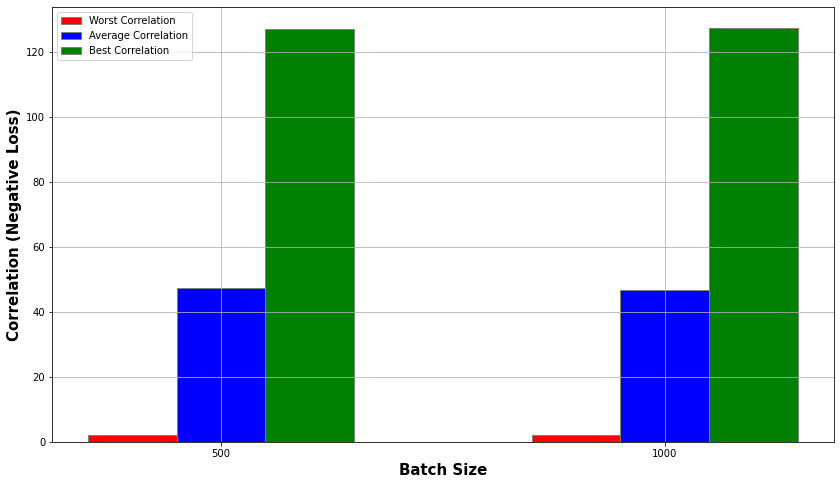
\includegraphics[width=\textwidth]{figures/DCCA_optimizations/NMF_Batch.png}
    \caption{\en{Batch size vs Achieved Correlation}}
\end{figure}
\begin{figure}[H]
    \centering
    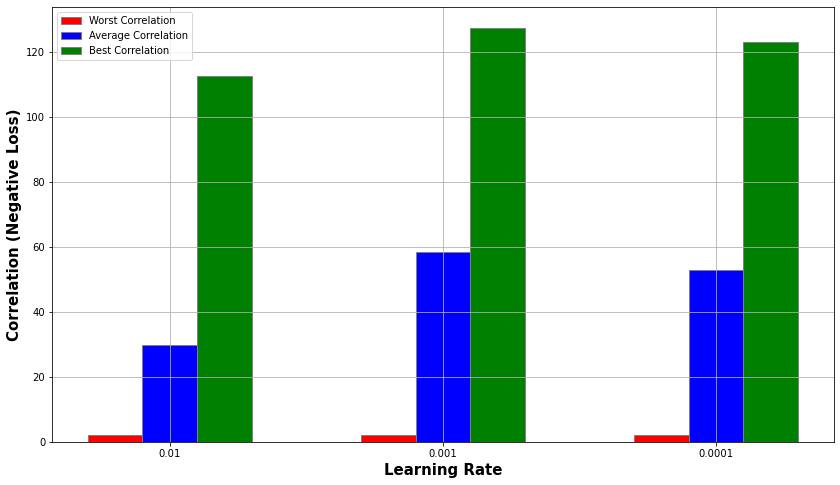
\includegraphics[width=\textwidth]{figures/DCCA_optimizations/NMF_Learning.png}
    \caption{\en{Learning Rate vs Achieved Correlation}}
\end{figure}
\begin{figure}[H]
    \centering
    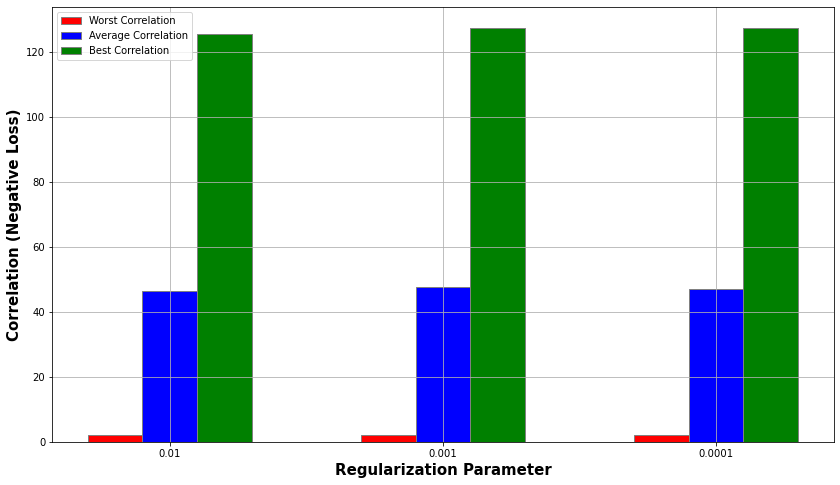
\includegraphics[width=\textwidth]{figures/DCCA_optimizations/NMF_Regularization.png}
    \caption{\en{Regularization Parameter vs Achieved Correlation}}
\end{figure}

Finally, in the case of the transformed through OPNMF imaging data combined with the raw genetic data, we can see that the parameter behaviour is again the same. Once again, output layer size increase correlates with better results, bigger hidden layer size, along with increasing the number of hidden layers improves the output correlation but only slightly, learning rate should be kept at a value of 0.001, and altering the other parameters has little to no effect.  

\begin{figure}[H]
    \centering
    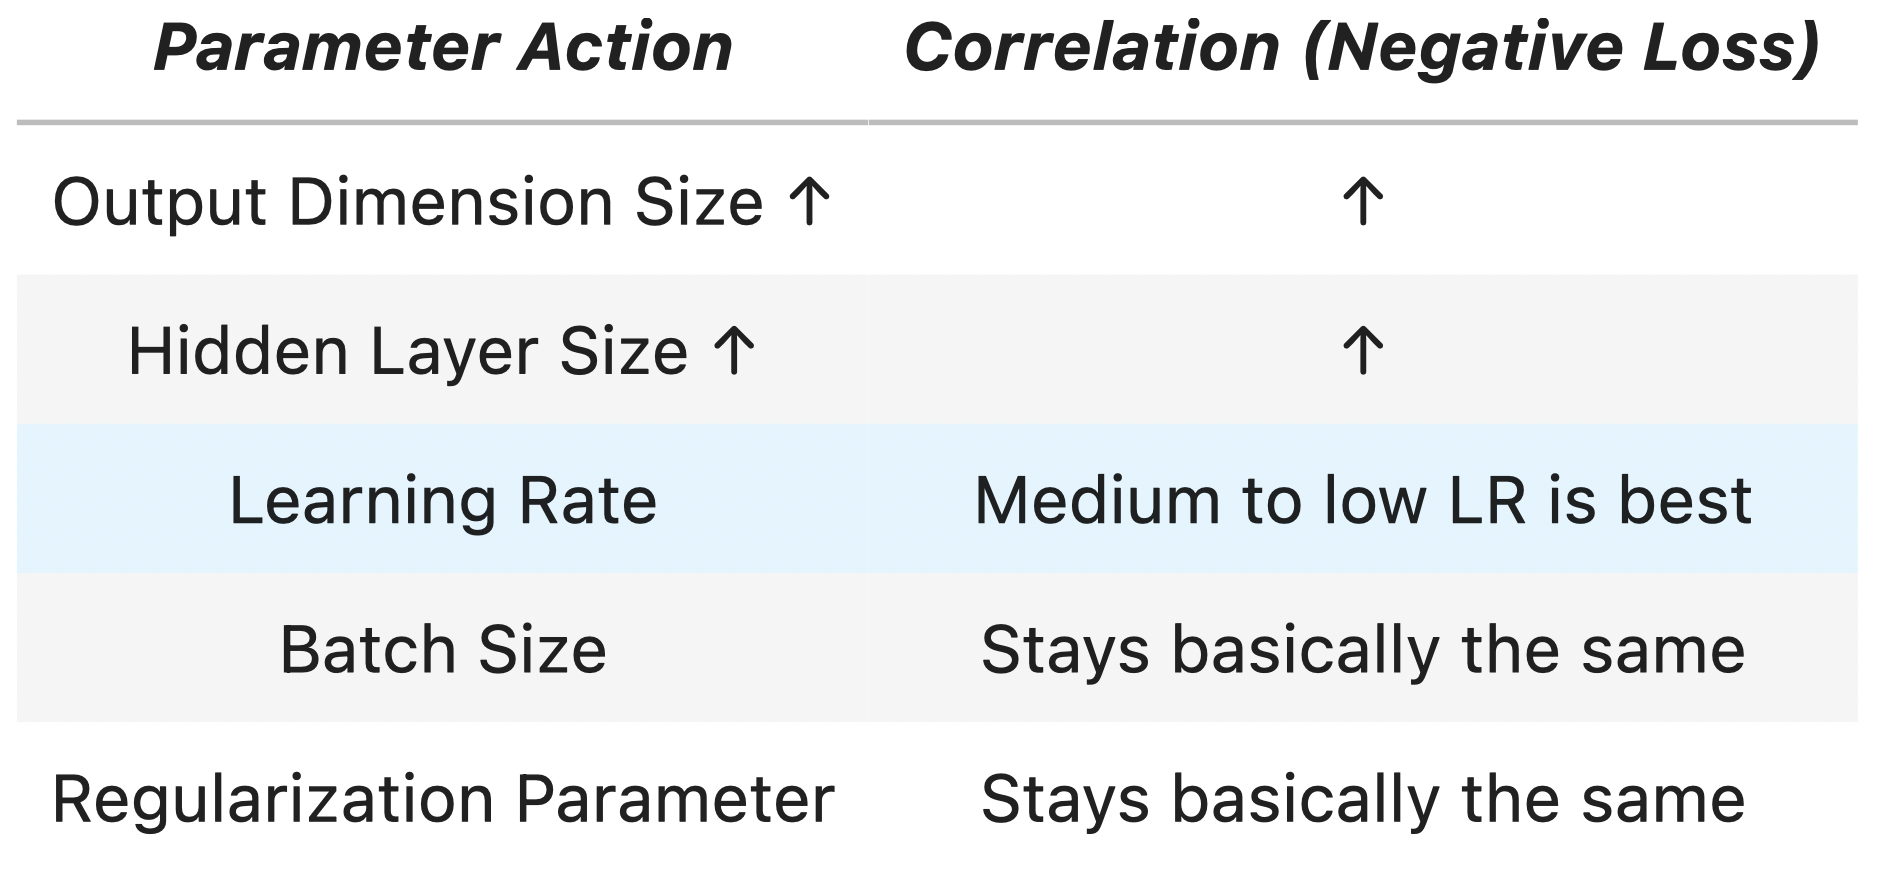
\includegraphics[width=0.7\textwidth]{figures/DCCA_optimizations/NMF_Conclusions.png}
    \caption{\en{Learned Conclusions from DCCA optimizations on 54 Imaging components and and 54 SNPs (Genetic)}}
\end{figure}
}
    %%%%%%% Results %%%%%%% 
    \chapter{\tl{Results} }
\en{In this chapter, we introduce results the methods and combinations thereof we experimented with achieved. 

First, the classification results of the raw views are presented, meaning the imaging data as is (145 ROIs) and the genetic data as is (54 SNPs), as a baseline. Those results are contrasted with the results of applying DCCA to those data. Following that, the classification results using MCA-transformed genetic data (10 genetic components) and the original imaging data are presented, and contrasted with DCCA applied on top of that. Afterwards, the respective results are presented after OPNMF (30 imaging components) and then with DCCA on top of that, using the combination of MCA and OPNMF, and finally after FAMD. 

For the aforementioned combinations of methods, the classification results are presented before and after scaling (if needed) and balancing, to highlight the effect those techniques have on the task. Finally, to ensure that the effect of having both views is properly documented, we perform the same task with both views, as well as keeping only one view, testing imaging and genetic for every method.

}
    \section{\tl{Raw data vs DCCA}}
\en{As mentioned before, we consider as the baseline results the SVM classification on the imaging and genetic data taken directly after LR on the ADNI dataset, and then compare them with the methods we experimented with. }
\subsection{\en{Without scaling or balancing:}}
\en{
\begin{figure}[H]
    \centering
    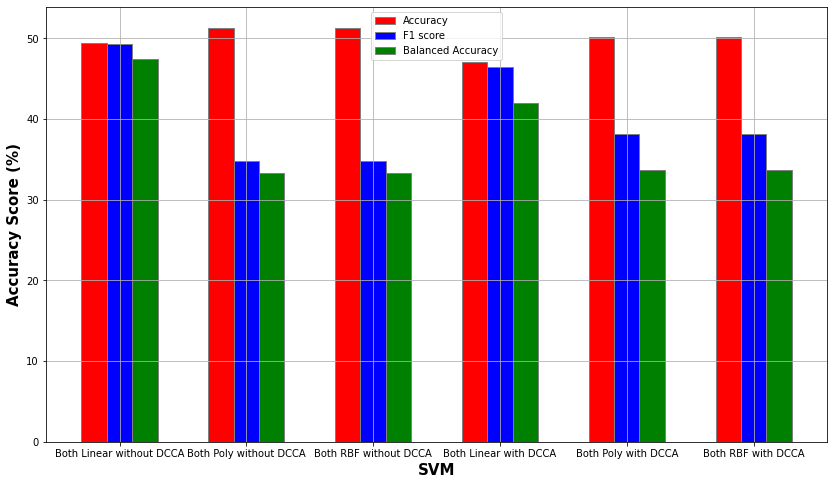
\includegraphics[width=\textwidth]{figures/Results/RAW/Raw_Both_out.png}
    \caption[\en{Classification metric scores using Both views on Raw vs DCCA data}]{\en{Classification metric scores using Both views (Imaging and Genetic), on the SVM kernels (Linear, Polynomial, RBF), using raw data (3 left bar groups) vs using DCCA (3 right bar groups)}}
\end{figure}

\begin{figure}[H]
    \centering
    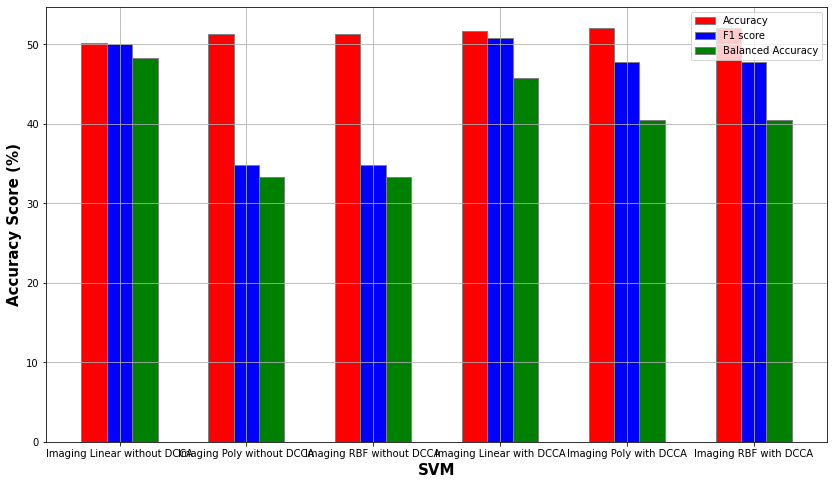
\includegraphics[width=\textwidth]{figures/Results/RAW/Raw_Ima_out.png}
    \caption[\en{Classification metric scores using Imaging view on Raw vs DCCA data}]{\en{Classification metric scores using only the Imaging view, on the SVM kernels (Linear, Polynomial, RBF), using raw data (3 left bar groups) vs using DCCA transformed imaging data, trained on both views (3 right bar groups)}}
\end{figure}

\begin{figure}[H]
    \centering
    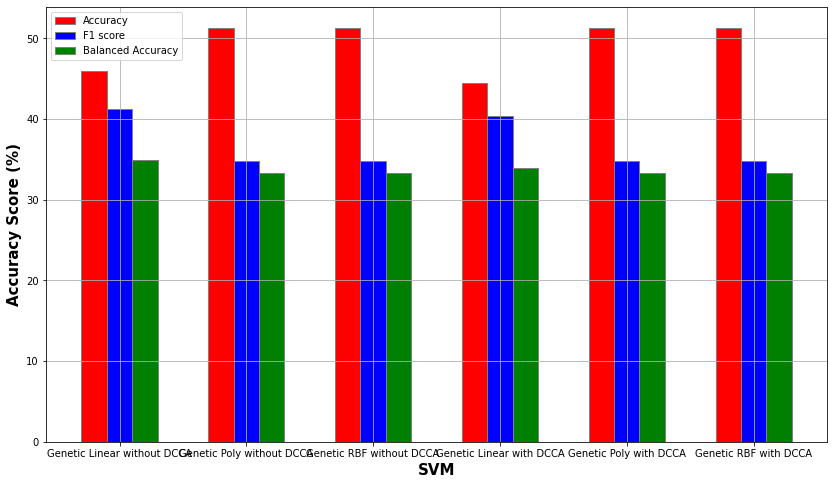
\includegraphics[width=\textwidth]{figures/Results/RAW/Raw_Gen_out.png}
    \caption[\en{Classification metric scores using Genetic view on Raw vs DCCA data}]{\en{Classification metric scores using only the Genetic view, on the SVM kernels (Linear, Polynomial, RBF), using raw data (3 left bar groups) vs using DCCA transformed genetic data, trained on both views (3 right bar groups)}}
\end{figure}

% \begin{figure}[H]
%     \centering
%     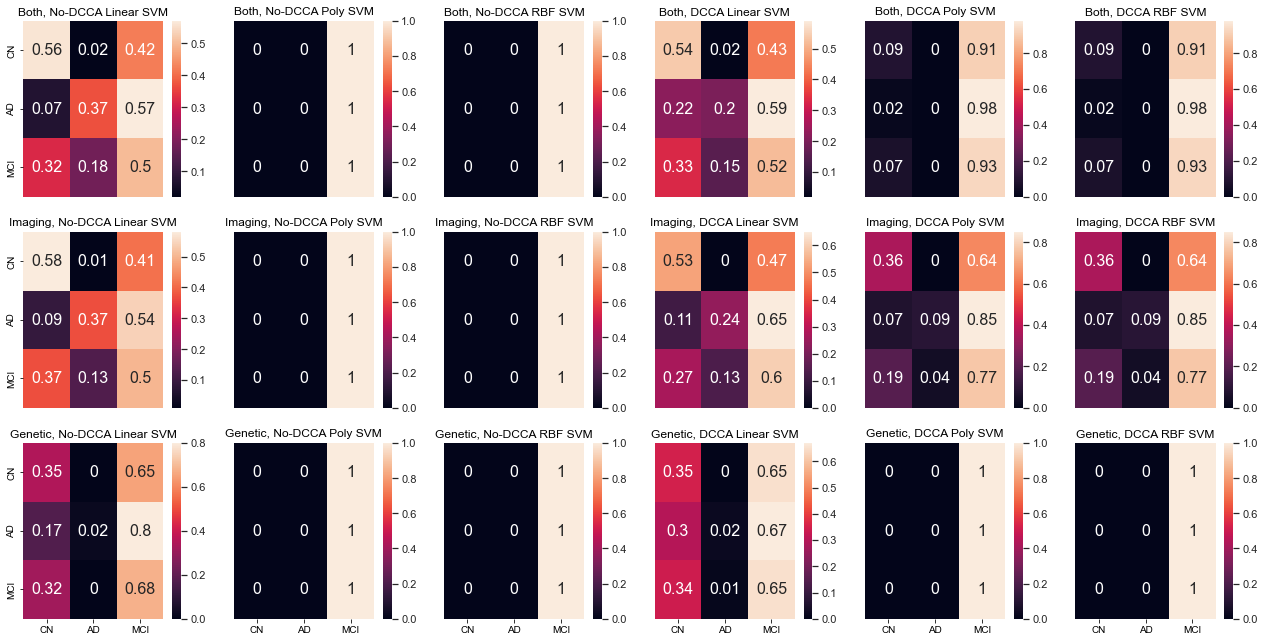
\includegraphics[width=\textwidth]{figures/Results/RAW/Raw_CM_out.png}
%     \caption[\en{Confusion Matrices of Raw vs DCCA data}]{\en{The Confusion Matrices for each class, per model, using both views (top row), only the imaging view (middle row), and only the genetic view (bottom row). The three left columns represent the CM of the raw data classification, while the three right columns represent the CM of the DCCA transformed data classification.}}
% \end{figure}

\begin{figure}[H]
    \centering
    \includegraphics[width=\textwidth]{figures/Results/RAW/Bagging_RAW_out.png}
    \caption[\en{Bagging Classification metrics}]{\en{Classification metric using Bagging on the imaging and genetic data.}}
\end{figure}

% \begin{figure}[H]
%     \centering
%     \includegraphics[width=\textwidth]{figures/Results/RAW/Bagging_RAW_CM_out.png}
%     \caption[\en{Bagging Confusion Matrices}]{\en{The Confusion Matrices for each class, with Bagging, for the imaging and genetic data.}}
% \end{figure}

\begin{figure}[H]
    \centering
    \includegraphics[width=\textwidth]{figures/Results/RAW/AdaBoost_RAW_out.png}
    \caption[\en{AdaBoost Classification metrics}]{\en{Classification metric using AdaBoost on the imaging and genetic data.}}
\end{figure}

% \begin{figure}[H]
%     \centering
%     \includegraphics[width=\textwidth]{figures/Results/RAW/AdaBoost_RAW_CM_out.png}
%     \caption[\en{AdaBoost Confusion Matrices}]{\en{The Confusion Matrices for each class, with AdaBoost, for the imaging and genetic data.}}
% \end{figure}

}
\subsection{\en{With scaling and balancing:}}
\en{
\begin{figure}[H]
    \centering
    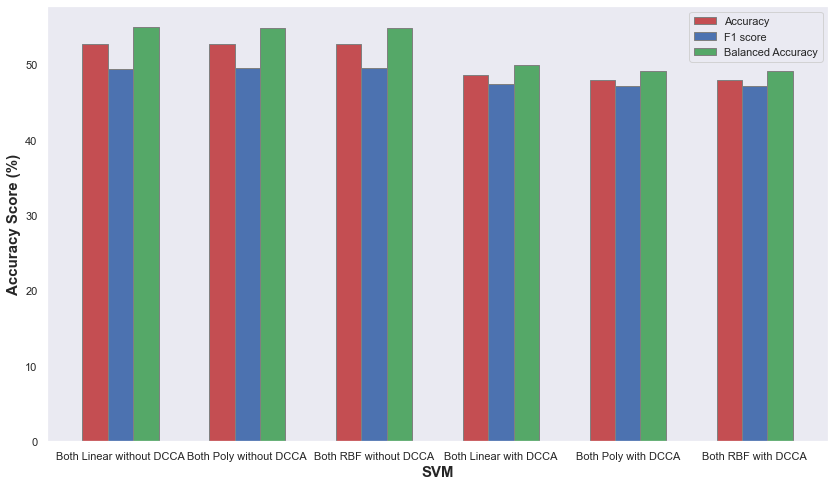
\includegraphics[width=\textwidth]{figures/Results/RAW/Raw_Both_with.png}
    \caption[\en{Classification metric scores using Both views on Raw vs DCCA data with scaling and balancing}]{\en{Classification metric scores using Both views (Imaging and Genetic), on the SVM kernels (Linear, Polynomial, RBF), using raw data (3 left bar groups) vs using DCCA (3 right bar groups)}}
\end{figure}

\begin{figure}[H]
    \centering
    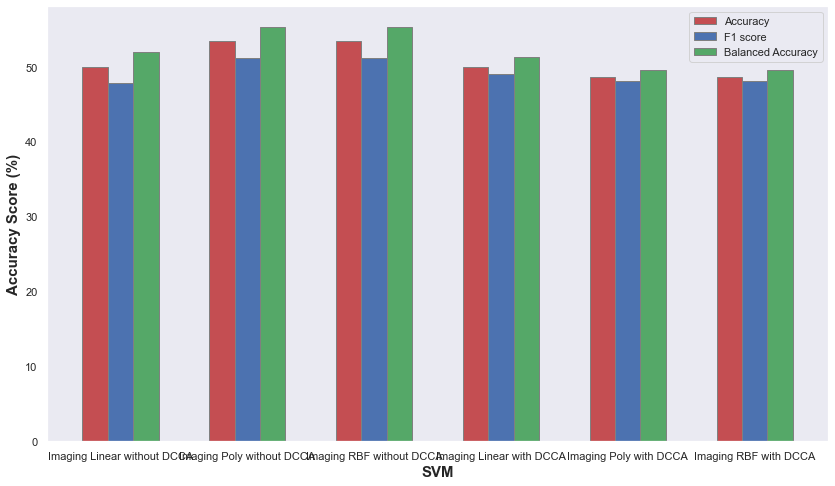
\includegraphics[width=\textwidth]{figures/Results/RAW/Raw_Ima_with.png}
    \caption[\en{Classification metric scores using Imaging view on Raw vs DCCA data with scaling and balancing}]{\en{Classification metric scores using only the Imaging view, on the SVM kernels (Linear, Polynomial, RBF), using raw data (3 left bar groups) vs using DCCA transformed imaging data, trained on both views (3 right bar groups)}}
\end{figure}

\begin{figure}[H]
    \centering
    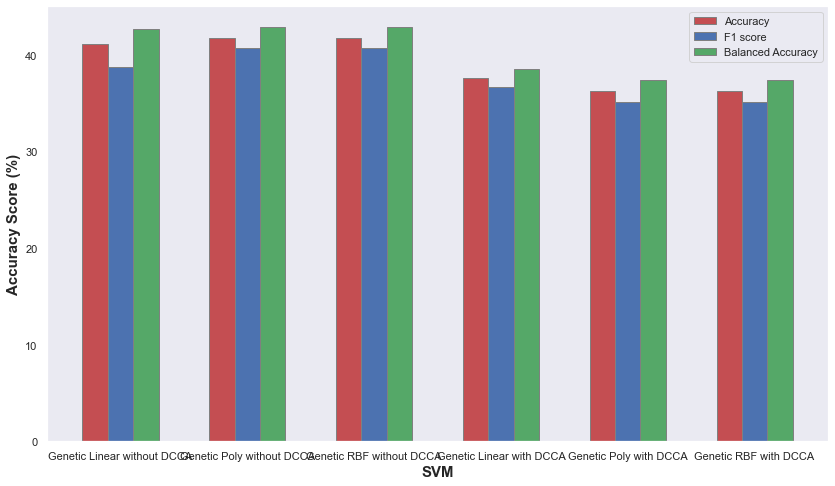
\includegraphics[width=\textwidth]{figures/Results/RAW/Raw_Gen_with.png}
    \caption[\en{Classification metric scores using Genetic view on Raw vs DCCA data with scaling and balancing}]{\en{Classification metric scores using only the Genetic view, on the SVM kernels (Linear, Polynomial, RBF), using raw data (3 left bar groups) vs using DCCA transformed genetic data, trained on both views (3 right bar groups)}}
\end{figure}

% \begin{figure}[H]
%     \centering
%     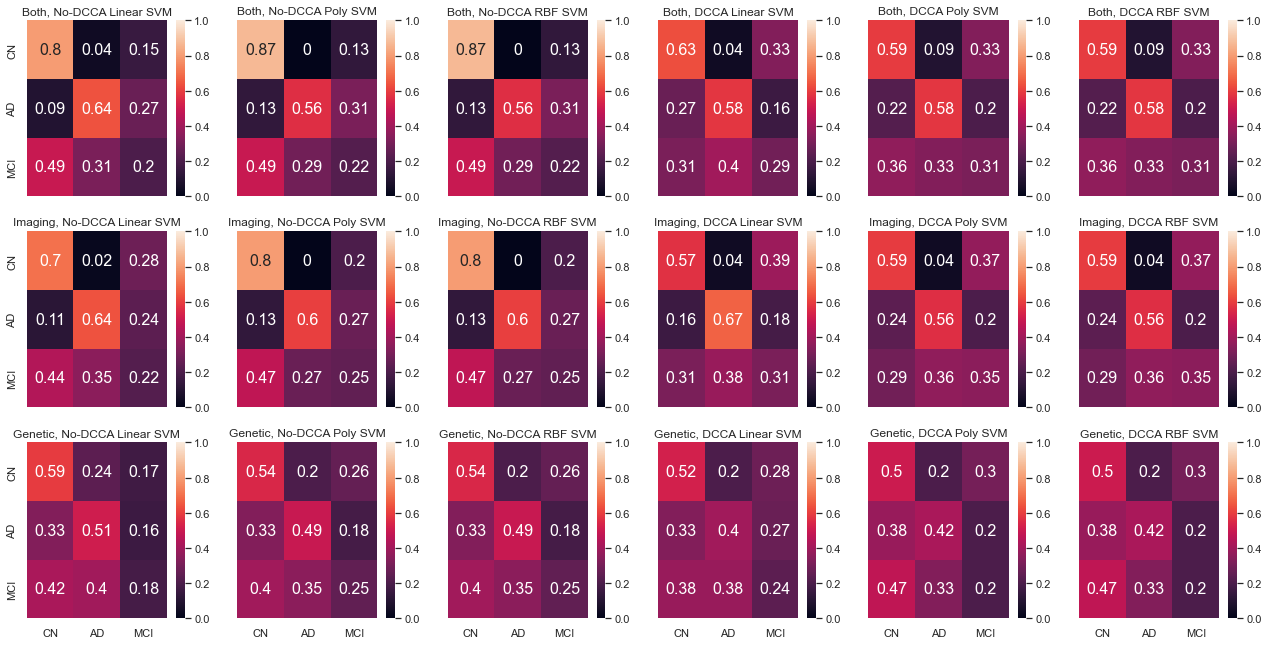
\includegraphics[width=\textwidth]{figures/Results/RAW/Raw_CM_with.png}
%     \caption[\en{Confusion Matrices of Raw vs DCCA data with scaling and balancing}]{\en{The Confusion Matrices for each class, per model, using both views (top row), only the imaging view (middle row), and only the genetic view (bottom row). The three left columns represent the CM of the raw data classification, while the three right columns represent the CM of the DCCA transformed data classification.}}
% \end{figure}

\begin{figure}[H]
    \centering
    \includegraphics[width=\textwidth]{figures/Results/RAW/Bagging_RAW_with.png}
    \caption[\en{Bagging Classification metrics with scaling and balancing}]{\en{Classification metric using Bagging on the imaging and genetic data.}}
\end{figure}

% \begin{figure}[H]
%     \centering
%     \includegraphics[width=\textwidth]{figures/Results/RAW/Bagging_RAW_CM_with.png}
%     \caption[\en{Bagging Confusion Matrices with scaling and balancing}]{\en{The Confusion Matrices for each class, with Bagging, for the imaging and genetic data.}}
% \end{figure}

\begin{figure}[H]
    \centering
    \includegraphics[width=\textwidth]{figures/Results/RAW/AdaBoost_RAW_with.png}
    \caption[\en{AdaBoost Classification metrics with scaling and balancing}]{\en{Classification metric using AdaBoost on the imaging and genetic data.}}
\end{figure}

% \begin{figure}[H]
%     \centering
%     \includegraphics[width=\textwidth]{figures/Results/RAW/AdaBoost_RAW_CM_with.png}
%     \caption[\en{AdaBoost Confusion Matrices with scaling and balancing}]{\en{The Confusion Matrices for each class, with AdaBoost, for the imaging and genetic data.}}
% \end{figure}

The following tables present the complete results for the raw data, as well as the DCCA transformed data, for each model, for each metric, for each view, and either with or without scaling and balancing. With green are highlighted the best values for each metric, depending on whether scaling and balancing were applied:

\begin{figure} [H]
    \centering
    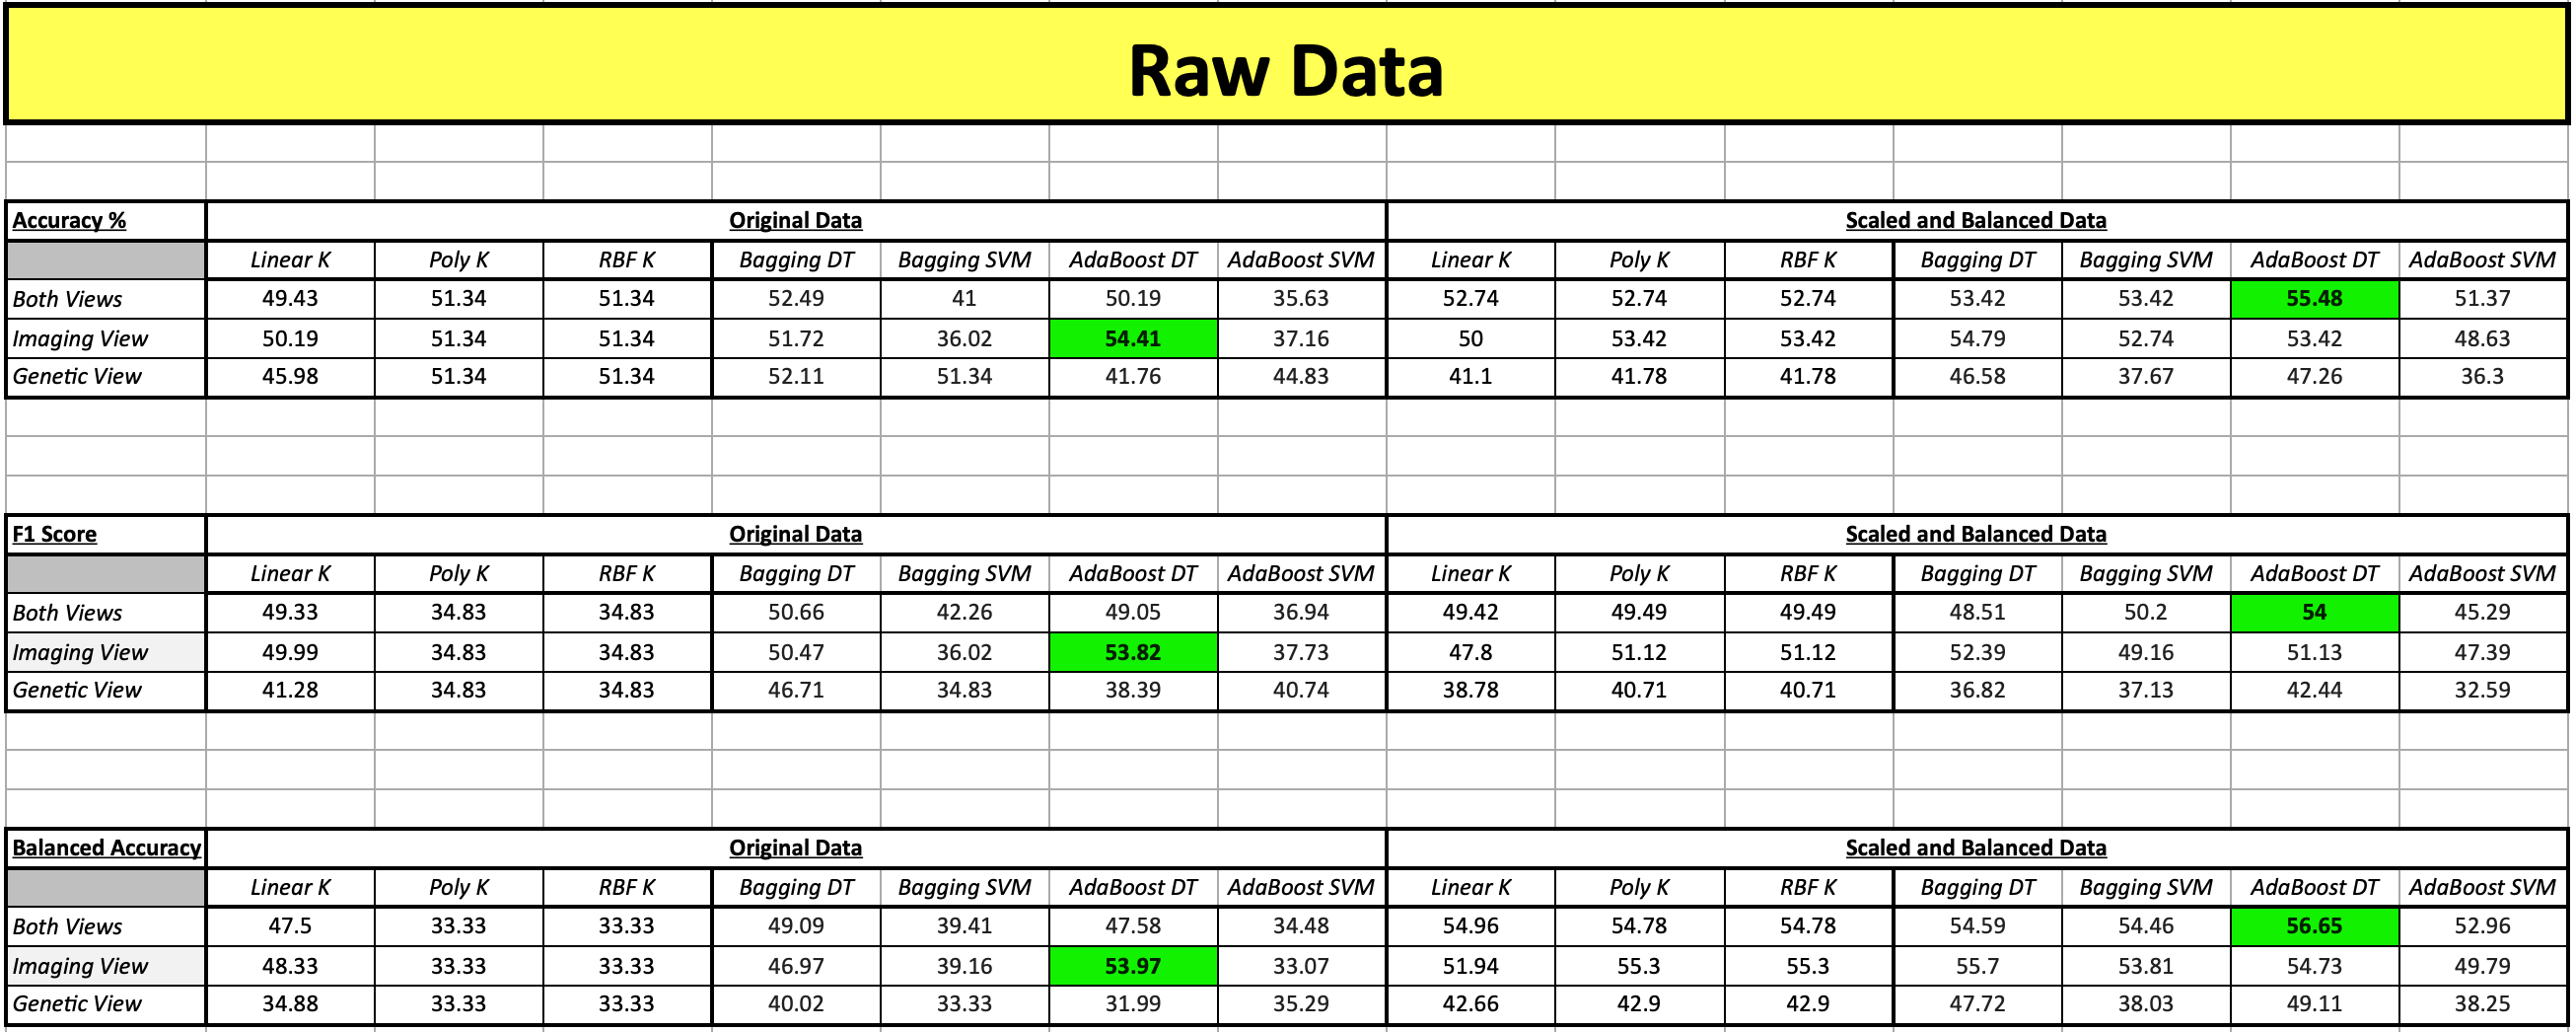
\includegraphics[width=\textwidth]{figures/Results/Analytical_Table_Raw.png}
    \caption[\en{Analytical table of results for raw data classification}]{\en{For each model and classifier, the metric scores for raw data classification are presented. Highlighted green are the best performing models, for each metric.}}
    \label{fig: Summary Table for classification scores for raw data}
\end{figure}

\begin{figure} [H]
    \centering
    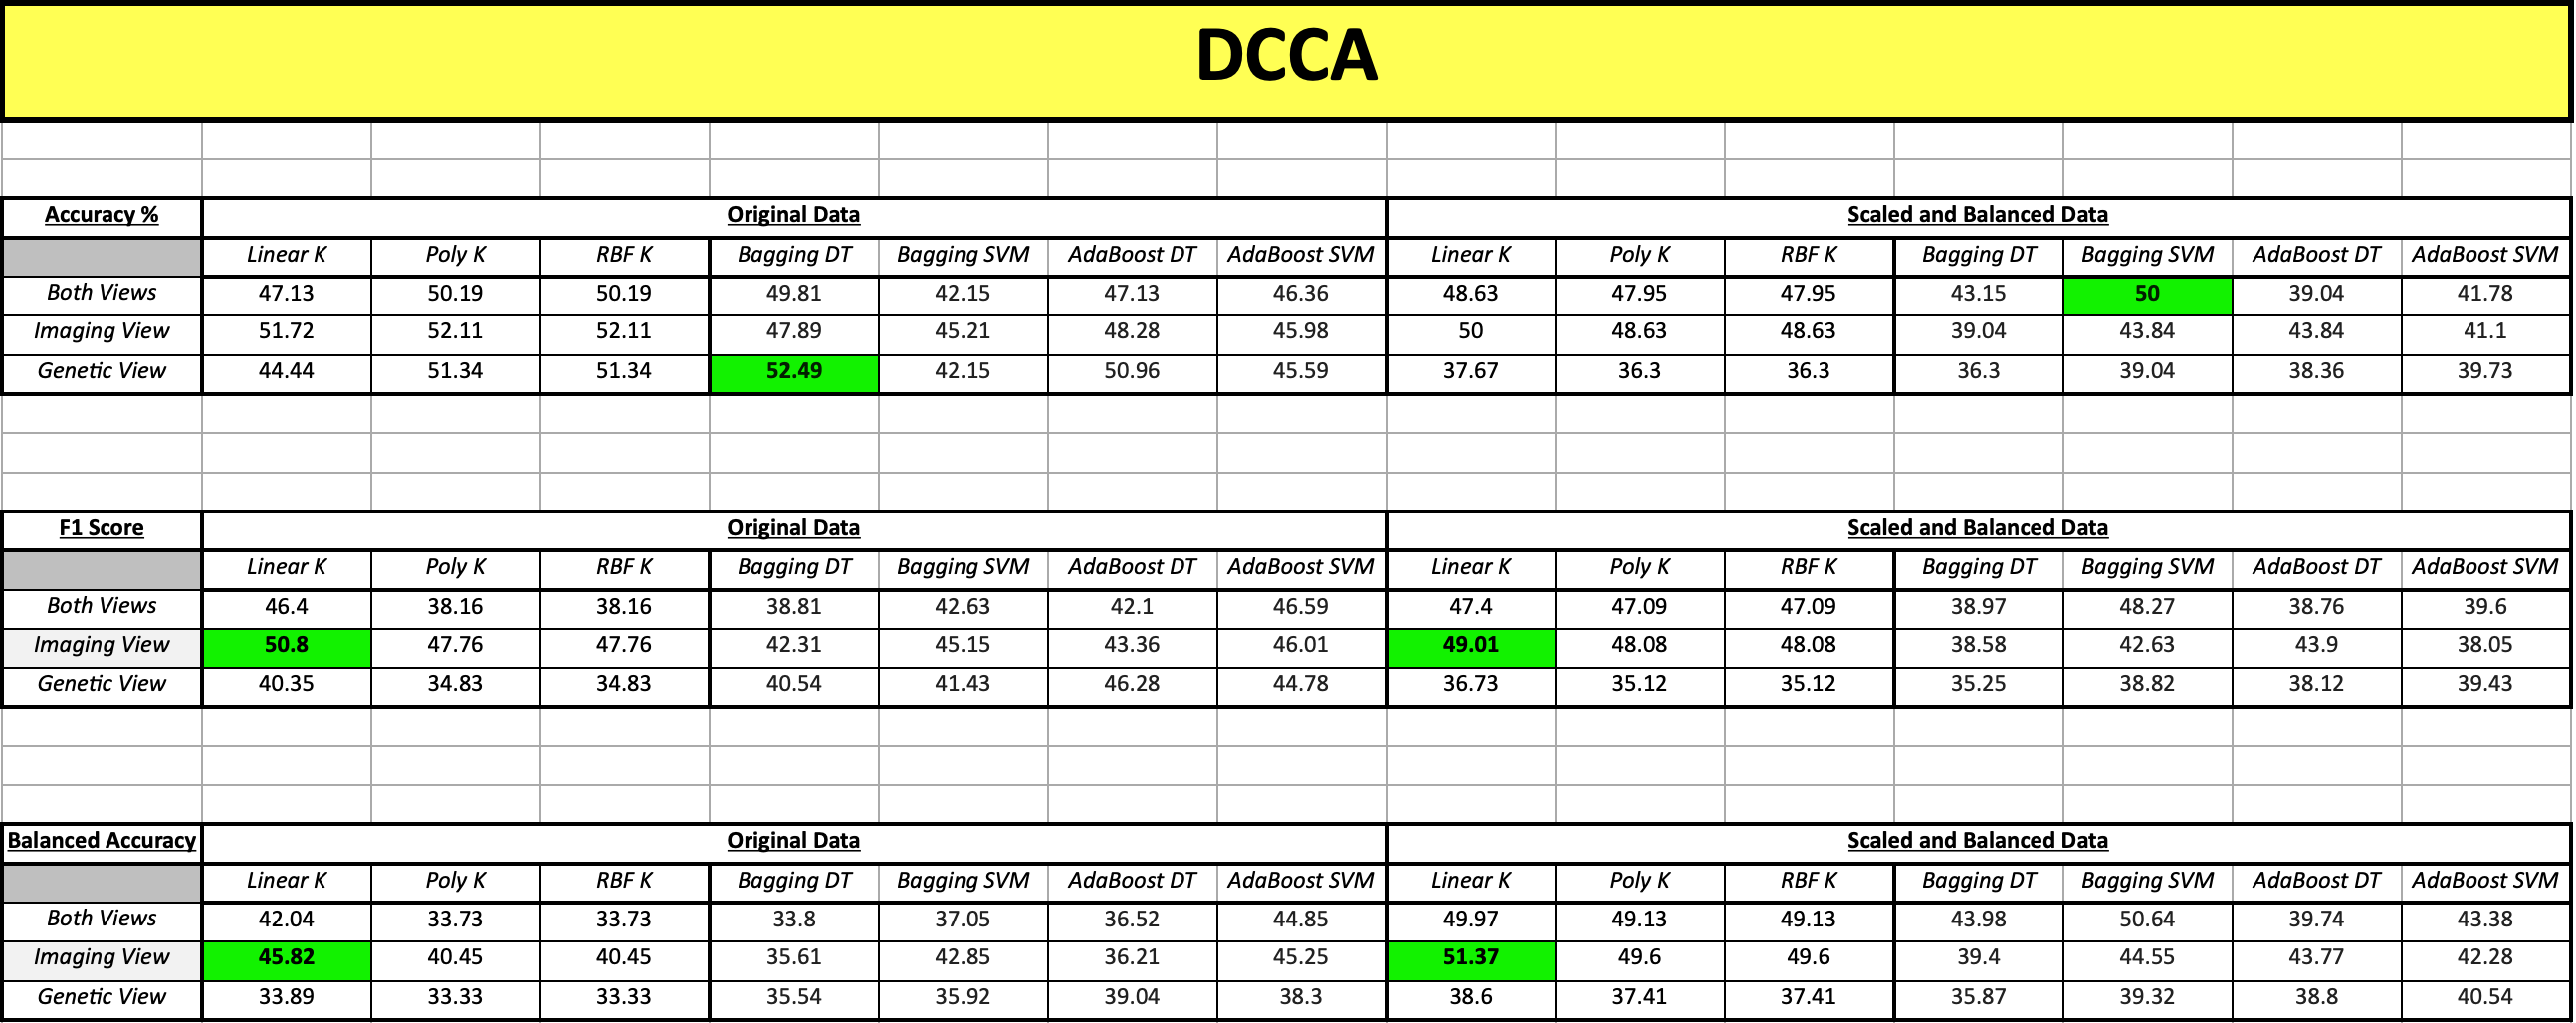
\includegraphics[width=\textwidth]{figures/Results/Analytical_Table_DCCA.png}
    \caption[\en{Analytical table of results for DCCA transformed data classification}]{\en{For each model and classifier, the metric scores for DCCA transformed data classification are presented. Highlighted green are the best performing models, for each metric.}}
    \label{fig: Summary Table for classification scores for DCCA data}
\end{figure}

}
    \section{\tl{MCA vs MCA - DCCA}}
\en{Moving on from the classification of the raw data versus the DCCA transformed data, we explore the effect that MCA has, and introduce the results of the classification. In this part, we present the classification results, (a) of the data after the genetic view has been transformed through MCA, and (b) of the DCCA transformed data after the genetic view has been transformed through MCA.}

\subsection{\en{Without scaling or balancing:}}
\en{
\begin{figure}[H]
    \centering
    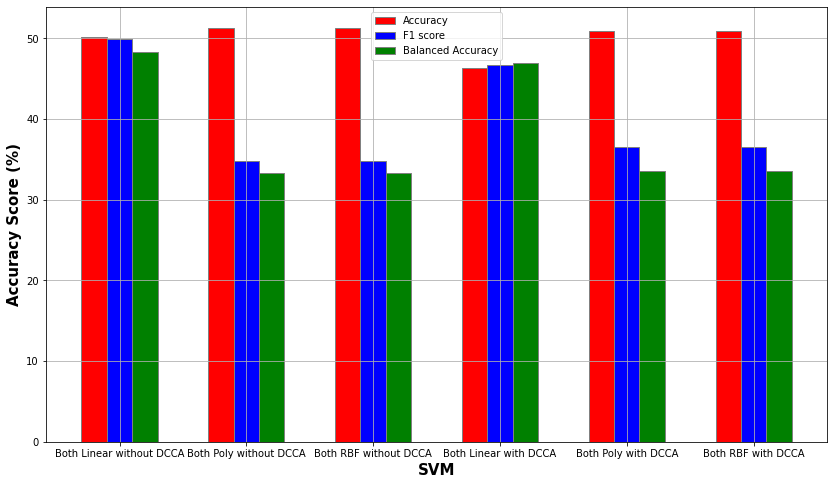
\includegraphics[width=\textwidth]{figures/Results/MCA/MCA_Both_out.png}
    \caption[\en{Classification metric scores using Both views on MCA vs MCA-DCCA data}]{\en{Classification metric scores using Both views (Imaging and Genetic), on the SVM kernels (Linear, Polynomial, RBF), using raw imaging and MCA transformed genetic data (3 left bar groups) vs using DCCA transformed raw imaging and MCA transformed genetic data (3 right bar groups)}}
\end{figure}

\begin{figure}[H]
    \centering
    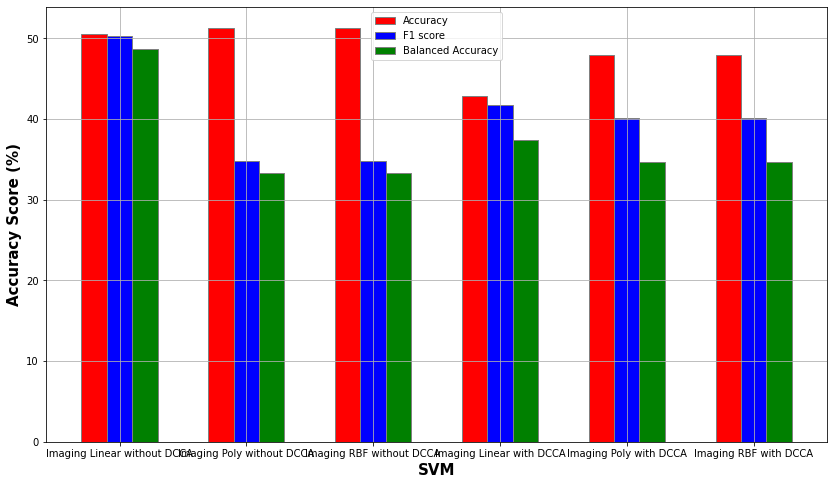
\includegraphics[width=\textwidth]{figures/Results/MCA/MCA_Ima_out.png}
    \caption[\en{Classification metric scores using Imaging view on MCA vs MCA-DCCA data}]{\en{Classification metric scores using only the Imaging view, on the SVM kernels (Linear, Polynomial, RBF), using raw imaging data (3 left bar groups) vs using the DCCA transformed imaging data, trained on raw imaging data and MCA transformed genetic data (3 right bar groups).}}
\end{figure}

\begin{figure}[H]
    \centering
    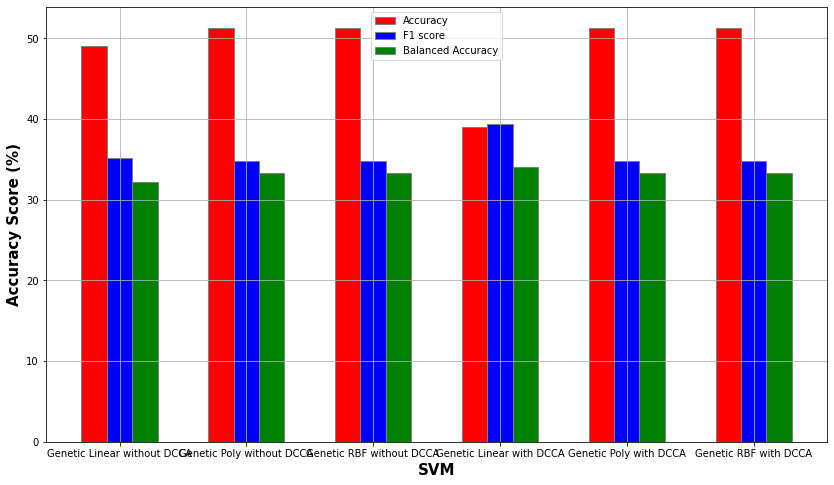
\includegraphics[width=\textwidth]{figures/Results/MCA/MCA_Gen_out.png}
    \caption[\en{Classification metric scores using Genetic view on MCA vs MCA-DCCA data}]{\en{Classification metric scores using only the genetic view, on the SVM kernels (Linear, Polynomial, RBF), using MCA transformed genetic data (3 left bar groups) vs using the DCCA transformed genetic data, trained on raw imaging data and MCA transformed genetic data (3 right bar groups).}}
\end{figure}

% \begin{figure}[H]
%     \centering
%     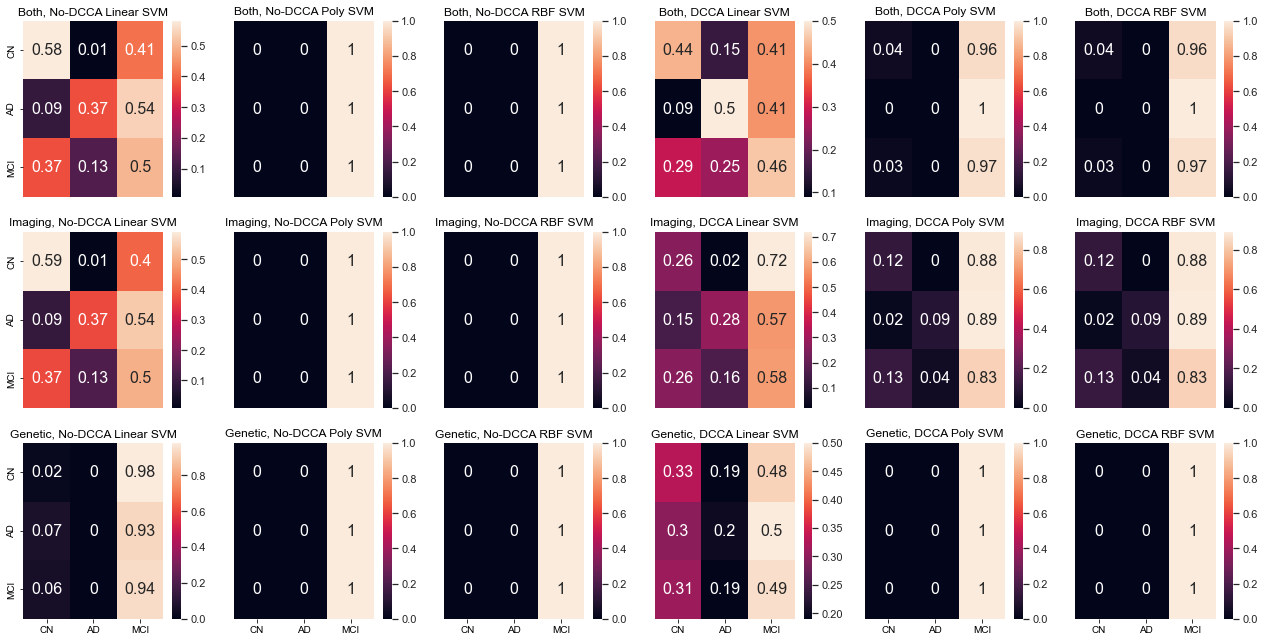
\includegraphics[width=\textwidth]{figures/Results/MCA/MCA_CM_out.png}
%     \caption[\en{Confusion Matrices of MCA vs MCA-DCCA data}]{\en{The Confusion Matrices for each class, per model, using both views (top row), only the imaging view (middle row), and only the genetic view (bottom row). The three left columns represent the CM of the raw imaging and MCA transformed genetic data classification, while the three right columns represent the CM of the DCCA transformed data classification.}}
% \end{figure}

\begin{figure}[H]
    \centering
    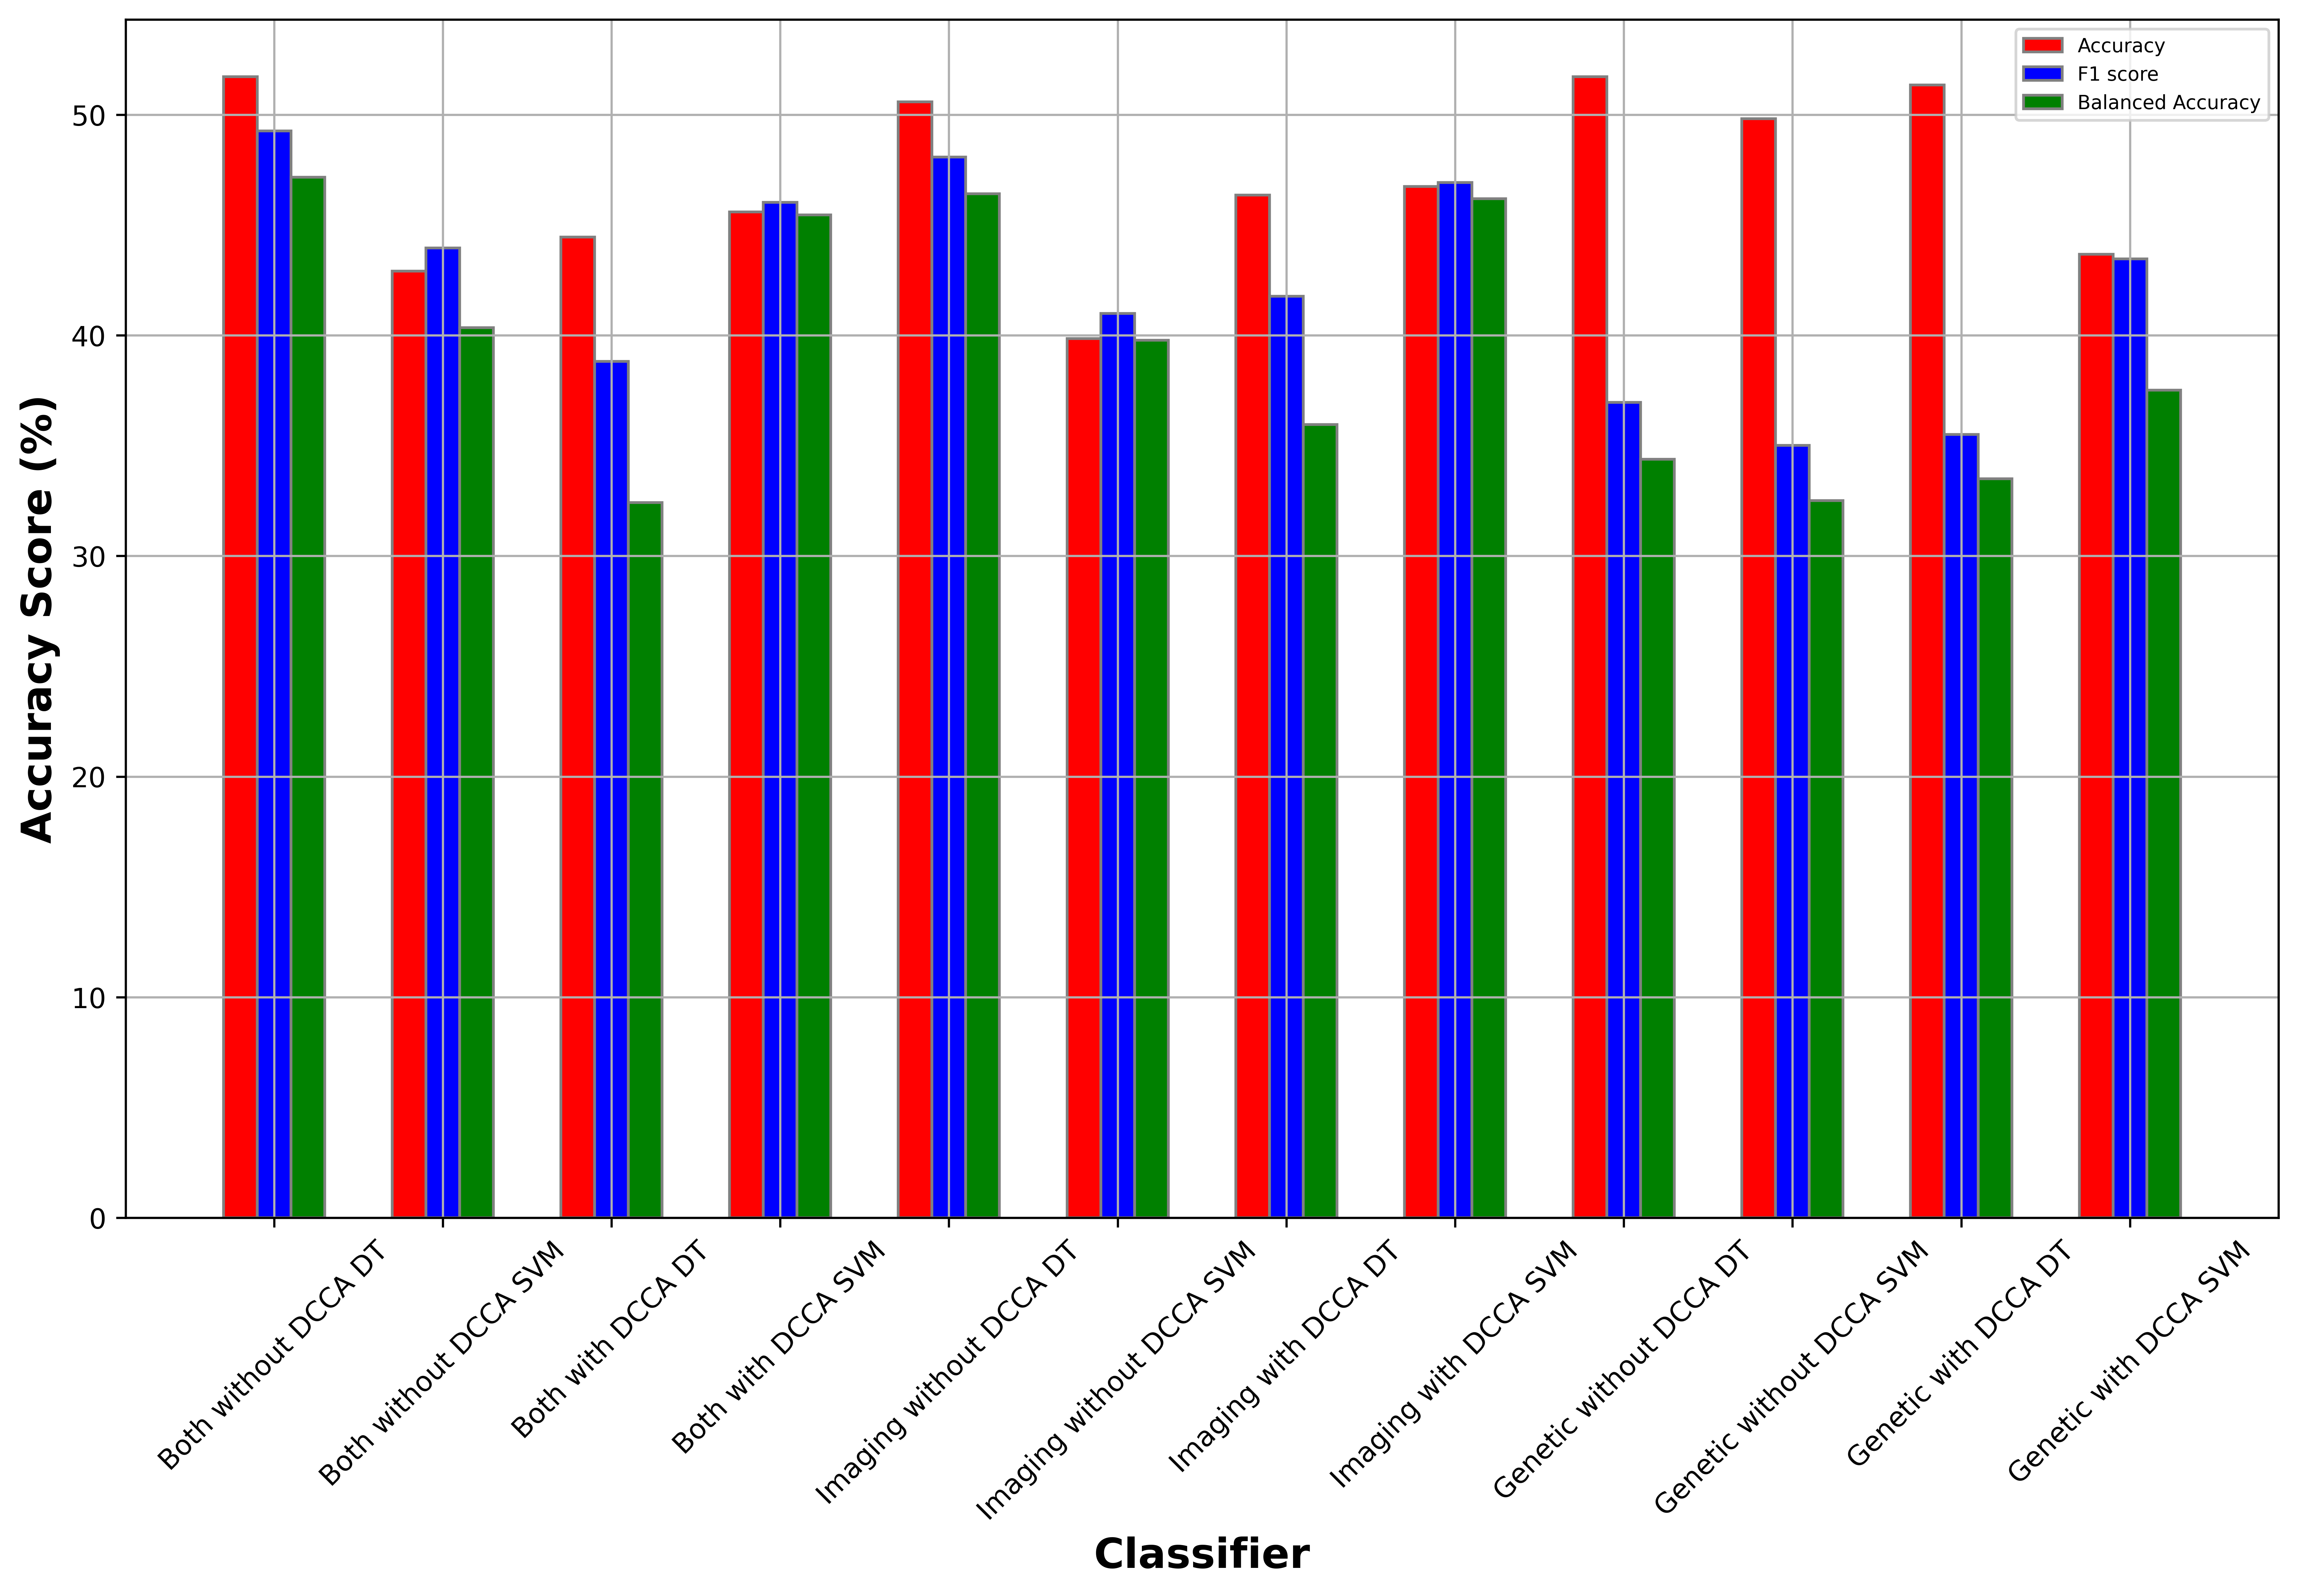
\includegraphics[width=\textwidth]{figures/Results/MCA/Bagging_MCA_out.png}
    \caption[\en{MCA Bagging Classification metrics}]{\en{Classification metric using Bagging on the MCA transformed imaging and genetic data.}}
\end{figure}

% \begin{figure}[H]
%     \centering
%     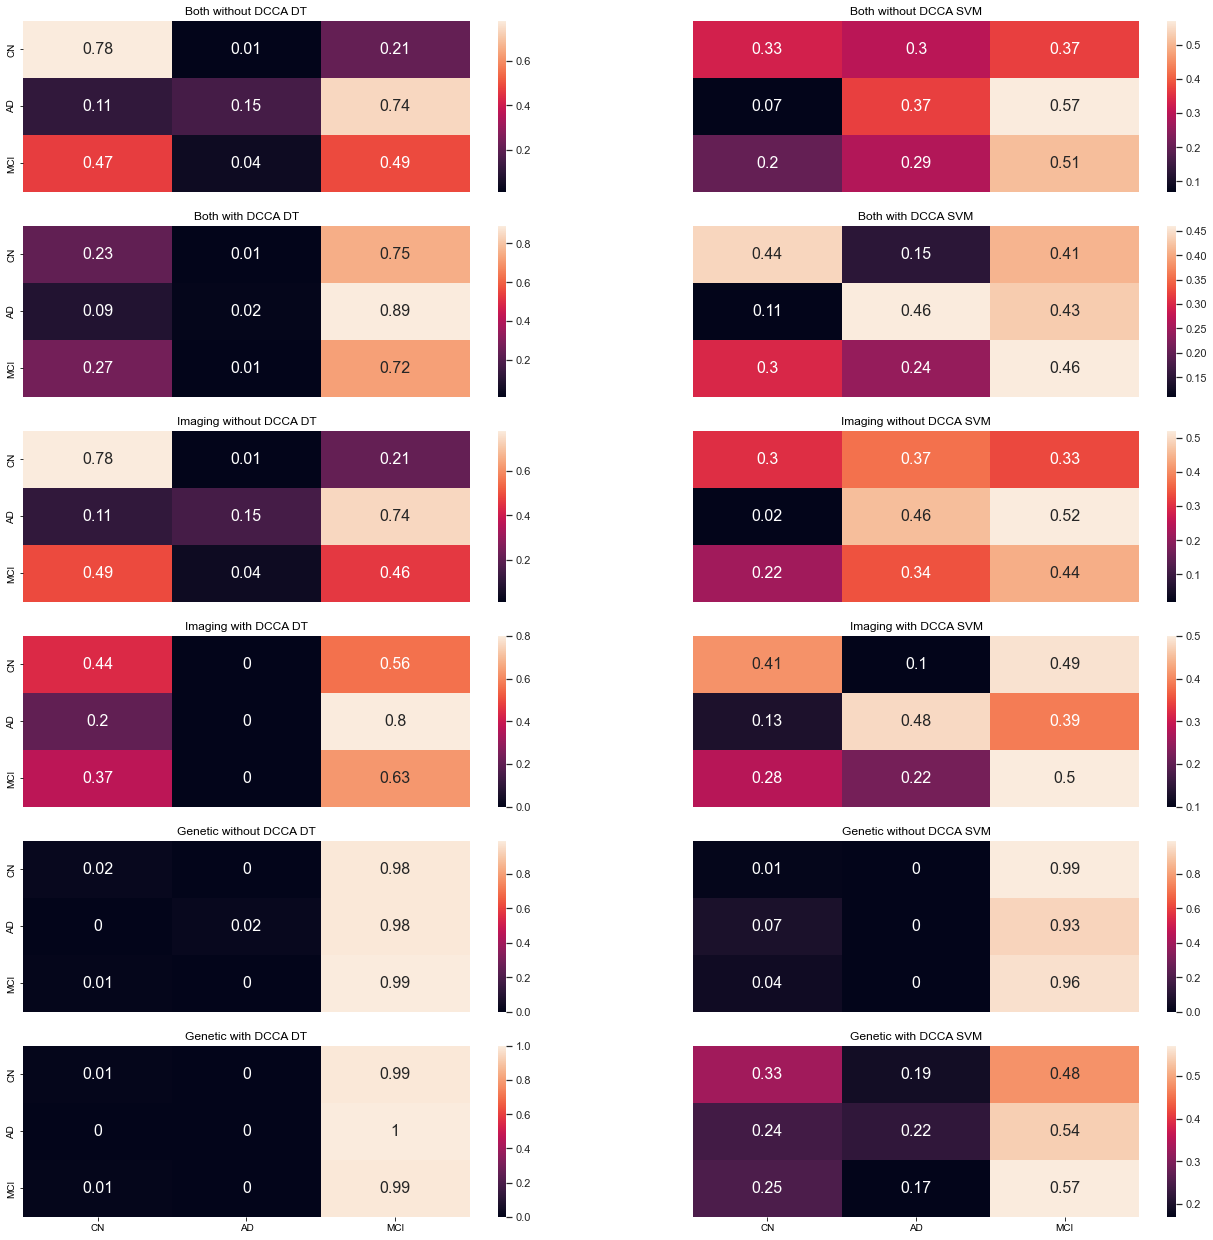
\includegraphics[width=\textwidth]{figures/Results/MCA/Bagging_MCA_CM_out.png}
%     \caption[\en{MCA Bagging Confusion Matrices}]{\en{The Confusion Matrices for each class, with Bagging, for the MCA transformed imaging and genetic data.}}
% \end{figure}

\begin{figure}[H]
    \centering
    \includegraphics[width=\textwidth]{figures/Results/MCA/AdaBoost_MCA_out.png}
    \caption[\en{MCA AdaBoost Classification metrics}]{\en{Classification metric using AdaBoost on the MCA transformed imaging and genetic data.}}
\end{figure}

% \begin{figure}[H]
%     \centering
%     \includegraphics[width=\textwidth]{figures/Results/MCA/AdaBoost_MCA_CM_out.png}
%     \caption[\en{MCA AdaBoost Confusion Matrices}]{\en{The Confusion Matrices for each class, with AdaBoost, for the MCA transformed imaging and genetic data.}}
% \end{figure}

}
\subsection{\en{With scaling and balancing:}}
\en{
\begin{figure}[H]
    \centering
    \includegraphics[width=\textwidth]{figures/Results/MCA/MCA_Both_with.png}
    \caption[\en{Classification metric scores using Both views on MCA vs MCA-DCCA data with scaling and balancing}]{\en{Classification metric scores using Both views (Imaging and Genetic), on the SVM kernels (Linear, Polynomial, RBF), using raw imaging and MCA transformed genetic data (3 left bar groups) vs using DCCA transformed raw imaging and MCA transformed genetic data (3 right bar groups)}}
\end{figure}

\begin{figure}[H]
    \centering
    \includegraphics[width=\textwidth]{figures/Results/MCA/MCA_Ima_with.png}
    \caption[\en{Classification metric scores using Imaging view on MCA vs MCA-DCCA data with scaling and balancing}]{\en{Classification metric scores using only the Imaging view, on the SVM kernels (Linear, Polynomial, RBF), using raw imaging data (3 left bar groups) vs using the DCCA transformed imaging data, trained on raw imaging data and MCA transformed genetic data (3 right bar groups).}}
\end{figure}

\begin{figure}[H]
    \centering
    \includegraphics[width=\textwidth]{figures/Results/MCA/MCA_Gen_with.png}
    \caption[\en{Classification metric scores using Genetic view on MCA vs MCA-DCCA data with scaling and balancing}]{\en{Classification metric scores using only the genetic view, on the SVM kernels (Linear, Polynomial, RBF), using MCA transformed genetic data (3 left bar groups) vs using the DCCA transformed genetic data, trained on raw imaging data and MCA transformed genetic data (3 right bar groups).}}
\end{figure}

The confusion matrices of the MCA and MCA - DCCA models are shown, because they performed exceptionally good:
\begin{figure}[H]
    \centering
    \includegraphics[width=\textwidth]{figures/Results/MCA/MCA_CM_with.png}
    \caption[\en{Confusion Matrices of MCA vs MCA-DCCA data with scaling and balancing}]{\en{The Confusion Matrices for each class, per model, using both views (top row), only the imaging view (middle row), and only the genetic view (bottom row). The three left columns represent the CM of the raw imaging and MCA transformed genetic data classification, while the three right columns represent the CM of the DCCA transformed data classification.}}
    \label{fig:Confusion Matrices of MCA vs MCA-DCCA data with scaling and balancing}
\end{figure}

\begin{figure}[H]
    \centering
    \includegraphics[width=\textwidth]{figures/Results/MCA/Bagging_MCA_with.png}
    \caption[\en{MCA Bagging Classification metrics with scaling and balancing}]{\en{Classification metric using Bagging on the MCA transformed imaging and genetic data.}}
\end{figure}

% \begin{figure}[H]
%     \centering
%     \includegraphics[width=\textwidth]{figures/Results/MCA/Bagging_MCA_CM_with.png}
%     \caption[\en{MCA Bagging Confusion Matrices with scaling and balancing}]{\en{The Confusion Matrices for each class, with Bagging, for the MCA transformed imaging and genetic data.}}
% \end{figure}

\begin{figure}[H]
    \centering
    \includegraphics[width=\textwidth]{figures/Results/MCA/AdaBoost_MCA_with.png}
    \caption[\en{MCA AdaBoost Classification metrics with scaling and balancing}]{\en{Classification metric using AdaBoost on the MCA transformed imaging and genetic data.}}
\end{figure}

% \begin{figure}[H]
%     \centering
%     \includegraphics[width=\textwidth]{figures/Results/MCA/AdaBoost_MCA_CM_with.png}
%     \caption[\en{MCA AdaBoost Confusion Matrices with scaling and balancing}]{\en{The Confusion Matrices for each class, with AdaBoost, for the MCA transformed imaging and genetic data.}}
% \end{figure}

The following tables present the complete results for the MCA transformed data, as well as the DCCA transformed data after MCA transformation on the genetic data, for each model, for each metric, for each view, and either with or without scaling and balancing. With green are highlighted the best values for each metric, depending on whether scaling and balancing were applied:

\begin{figure} [H]
    \centering
    \includegraphics[width=\textwidth]{figures/Results/Analytical_Table_MCA.png}
    \caption[\en{Analytical table of results for MCA data classification}]{\en{For each model and classifier, the metric scores for MCA transformed data classification are presented. Highlighted green are the best performing models, for each metric.}}
    \label{fig: Summary Table for classification scores for MCA transformed data}
\end{figure}

\begin{figure} [H]
    \centering
    \includegraphics[width=\textwidth]{figures/Results/Analytical_Table_MCA_DCCA.png}
    \caption[\en{Analytical table of results for MCA-DCCA transformed data classification}]{\en{For each model and classifier, the metric scores for MCA - DCCA transformed data classification are presented. Highlighted green are the best performing models, for each metric.}}
    \label{fig: Summary Table for classification scores for MCA - DCCA transformed data}
\end{figure}

}
    \section{\tl{OPNMF vs OPNMF - DCCA}}
\en{
Furthermore, we explore the effect that OPNMF has to the task of classification. To that extent, we compare the classification results of (a) the data after the imaging view has been transformed with OPNMF and (b) the DCCA transformed data, trained on the raw genetic data and the OPNMF transformed imaging data.

}
\subsection{\en{Without scaling or balancing:}}
\en{
\begin{figure}[H]
    \centering
    \includegraphics[width=\textwidth]{figures/Results/NMF/NMF_Both_out.png}
    \caption[\en{Classification metric scores using Both views on OPNMF vs OPNMF-DCCA data}]{\en{Classification metric scores using Both views (Imaging and Genetic), on the SVM kernels (Linear, Polynomial, RBF), using raw genetic and OPNMF transformed imaging data (3 left bar groups) vs using DCCA transformed raw genetic and OPNMF transformed imaging data (3 right bar groups)}}
\end{figure}

\begin{figure}[H]
    \centering
    \includegraphics[width=\textwidth]{figures/Results/NMF/NMF_Ima_out.png}
    \caption[\en{Classification metric scores using Imaging view on OPNMF vs OPNMF-DCCA data}]{\en{Classification metric scores using only the Imaging view, on the SVM kernels (Linear, Polynomial, RBF), using OPNMF transformed imaging data (3 left bar groups) vs using the DCCA transformed imaging data, trained on raw genetic data and OPNMF transformed genetic data (3 right bar groups).}}
\end{figure}

\begin{figure}[H]
    \centering
    \includegraphics[width=\textwidth]{figures/Results/NMF/NMF_Gen_out.png}
    \caption[\en{Classification metric scores using Genetic view on OPNMF vs OPNMF-DCCA data}]{\en{Classification metric scores using only the Imaging view, on the SVM kernels (Linear, Polynomial, RBF), using OPNMF transformed imaging data (3 left bar groups) vs using the DCCA transformed imaging data, trained on raw genetic data and OPNMF transformed genetic data (3 right bar groups).}}
\end{figure}

% \begin{figure}[H]
%     \centering
%     \includegraphics[width=\textwidth]{figures/Results/NMF/NMF_CM_out.png}
%     \caption[\en{Confusion Matrices of OPNMF vs OPNMF-DCCA data}]{\en{Classification metric scores using only the Imaging view, on the SVM kernels (Linear, Polynomial, RBF), using OPNMF transformed imaging data (3 left bar groups) vs using the DCCA transformed imaging data, trained on raw genetic data and OPNMF transformed genetic data (3 right bar groups).}}
% \end{figure}

\begin{figure}[H]
    \centering
    \includegraphics[width=\textwidth]{figures/Results/NMF/Bagging_NMF_out.png}
    \caption[\en{OPNMF Bagging Classification metrics}]{\en{Classification metric using Bagging on the OPNMF transformed imaging and genetic data.}}
\end{figure}

% \begin{figure}[H]
%     \centering
%     \includegraphics[width=\textwidth]{figures/Results/NMF/Bagging_NMF_CM_out.png}
%     \caption[\en{OPNMF Bagging Confusion Matrices}]{\en{The Confusion Matrices for each class, with Bagging, for the OPNMF transformed imaging and genetic data.}}
% \end{figure}

\begin{figure}[H]
    \centering
    \includegraphics[width=\textwidth]{figures/Results/NMF/AdaBoost_NMF_out.png}
    \caption[\en{OPNMF AdaBoost Classification metrics}]{\en{Classification metric using AdaBoost on the OPNMF transformed imaging and genetic data.}}
\end{figure}

% \begin{figure}[H]
%     \centering
%     \includegraphics[width=\textwidth]{figures/Results/NMF/AdaBoost_NMF_CM_out.png}
%     \caption[\en{OPNMF AdaBoost Confusion Matrices}]{\en{The Confusion Matrices for each class, with AdaBoost, for the OPNMF transformed imaging and genetic data.}}
% \end{figure}
}
\subsection{\en{With scaling and balancing:}}
\en{
\begin{figure}[H]
    \centering
    \includegraphics[width=\textwidth]{figures/Results/NMF/NMF_Both_with.png}
    \caption[\en{Classification metric scores using Both views on OPNMF vs OPNMF-DCCA data }]{\en{Classification metric scores using Both views (Imaging and Genetic), on the SVM kernels (Linear, Polynomial, RBF), using raw genetic and OPNMF transformed imaging data (3 left bar groups) vs using DCCA transformed raw genetic and OPNMF transformed imaging data (3 right bar groups)}}
\end{figure}

\begin{figure}[H]
    \centering
    \includegraphics[width=\textwidth]{figures/Results/NMF/NMF_Ima_with.png}
    \caption[\en{Classification metric scores using Imaging view on OPNMF vs OPNMF-DCCA data }]{\en{Classification metric scores using only the Imaging view, on the SVM kernels (Linear, Polynomial, RBF), using OPNMF transformed imaging data (3 left bar groups) vs using the DCCA transformed imaging data, trained on raw genetic data and OPNMF transformed genetic data (3 right bar groups).}}
\end{figure}

\begin{figure}[H]
    \centering
    \includegraphics[width=\textwidth]{figures/Results/NMF/NMF_Gen_with.png}
    \caption[\en{Classification metric scores using Genetic view on OPNMF vs OPNMF-DCCA data }]{\en{Classification metric scores using only the genetic view, on the SVM kernels (Linear, Polynomial, RBF), using raw genetic data (3 left bar groups) vs using the DCCA transformed genetic data, trained on raw genetic data and OPNMF transformed imaging data (3 right bar groups).}}
\end{figure}

% \begin{figure}[H]
%     \centering
%     \includegraphics[width=\textwidth]{figures/Results/NMF/NMF_CM_with.png}
%     \caption[\en{Confusion Matrices of OPNMF vs OPNMF-DCCA data with scaling and balancing}]{\en{The Confusion Matrices for each class, per model, using both views (top row), only the imaging view (middle row), and only the genetic view (bottom row). The three left columns represent the CM of the raw genetic and OPNMF transformed imaging data classification, while the three right columns represent the CM of the DCCA transformed data classification.}}
% \end{figure}

\begin{figure}[H]
    \centering
    \includegraphics[width=\textwidth]{figures/Results/NMF/Bagging_NMF_with.png}
    \caption[\en{OPNMF Bagging Classification metrics with scaling and balancing}]{\en{Classification metric using Bagging on the OPNMF transformed imaging and genetic data.}}
\end{figure}

\begin{figure}[H]
    \centering
    \includegraphics[width=\textwidth]{figures/Results/NMF/AdaBoost_NMF_with.png}
    \caption[\en{OPNMF AdaBoost Classification metrics with scaling and balancing}]{\en{Classification metric using AdaBoost on the OPNMF transformed imaging and genetic data.}}
\end{figure}

The confusion matrices of the OPNMF Bagging models are shown, because they performed exceptionally good:
\begin{figure}[H]
    \centering
    \includegraphics[width=\textwidth]{figures/Results/NMF/Bagging_NMF_CM_with.png}
    \caption[\en{OPNMF Bagging Confusion Matrices with scaling and balancing}]{\en{The Confusion Matrices for each class, with Bagging, for the OPNMF transformed imaging and genetic data.}}
    \label{fig:OPNMF Bagging Confusion Matrices with scaling and balancing}
\end{figure}

\begin{figure}[H]
    \centering
    \includegraphics[width=\textwidth]{figures/Results/NMF/AdaBoost_NMF_CM_with.png}
    \caption[\en{OPNMF AdaBoost Confusion Matrices with scaling and balancing}]{\en{The Confusion Matrices for each class, with AdaBoost, for the OPNMF transformed imaging and genetic data.}}
    \label{fig:OPNMF AdaBoost Confusion Matrices with scaling and balancing}
\end{figure}

The following tables present the complete results for the OPNMF transformed data, as well as the DCCA transformed data after OPMNF transformation on the imaging data, for each model, for each metric, for each view, and either with or without scaling and balancing. With green are highlighted the best values for each metric, depending on whether scaling and balancing were applied:

\begin{figure} [H]
    \centering
    \includegraphics[width=\textwidth]{figures/Results/Analytical_Table_OPNMF.png}
    \caption[\en{Analytical table of results for OPNMF data classification}]{\en{For each model and classifier, the metric scores for OPNMF transformed data classification are presented. Highlighted green are the best performing models, for each metric.}}
    \label{fig: Summary Table for classification scores for OPNMF transformed data}
\end{figure}

\begin{figure} [H]
    \centering
    \includegraphics[width=\textwidth]{figures/Results/Analytical_Table_OPNMF_DCCA.png}
    \caption[\en{Analytical table of results for OPNMF - DCCA transformed data classification}]{\en{For each model and classifier, the metric scores for OPNMF - DCCA transformed data classification are presented. Highlighted green are the best performing models, for each metric.}}
    \label{fig: Summary Table for classification scores for OPNMF - DCCA transformed data}
\end{figure}
}
    \section{\tl{Application of MCA to the genetic data along with OPNMF to the imaging data}}
\en{Combining the two previous techniques, we now apply MCA to the genetic data, and OPNMF to the imaging data, and combine the two transformed views for the classification task. 
}
\subsection{\en{Without scaling or balancing:}}
\en{
\begin{figure}[H]
    \centering
    \includegraphics[width=\textwidth]{figures/Results/MCA_NMF/MCA_NMF_out.png}
    \caption[\en{MCA OPNMF Classification metrics}]{\en{Classification metric using both views (imaging and genetic) on the SVM kernels (Linear, Polynomial, RBF), using the MCA transformed genetic and OPNMF transformed imaging data.}}
\end{figure}

% \begin{figure}[H]
%     \centering
%     \includegraphics[width=\textwidth]{figures/Results/MCA_NMF/MCA_NMF_CM_out.png}
%     \caption[\en{MCA OPNMF Confusion Matrices}]{\en{The Confusion Matrices for each class, per SVM kernel, for the MCA transformed genetic and OPNMF transformed imaging data.}}
% \end{figure}

\begin{figure}[H]
    \centering
    \includegraphics[width=\textwidth]{figures/Results/MCA_NMF/Bagging_MCAOPNMF_out.png}
    \caption[\en{MCA and OPNMF Bagging Classification metrics}]{\en{Classification metric using Bagging on the MCA and OPNMF transformed imaging and genetic data.}}
\end{figure}

% \begin{figure}[H]
%     \centering
%     \includegraphics[width=\textwidth]{figures/Results/MCA_NMF/Bagging_MCAOPNMF_CM_out.png}
%     \caption[\en{MCA and OPNMF Bagging Confusion Matrices}]{\en{The Confusion Matrices for each class, with Bagging, for the MCA and OPNMF transformed imaging and genetic data.}}
% \end{figure}

\begin{figure}[H]
    \centering
    \includegraphics[width=\textwidth]{figures/Results/MCA_NMF/AdaBoost_MCAOPNMF_out.png}
    \caption[\en{MCA and OPNMF AdaBoost Classification metrics}]{\en{Classification metric using AdaBoost on the MCA and OPNMF transformed imaging and genetic data.}}
\end{figure}

% \begin{figure}[H]
%     \centering
%     \includegraphics[width=\textwidth]{figures/Results/MCA_NMF/AdaBoost_MCAOPNMF_CM_out.png}
%     \caption[\en{MCA and OPNMF AdaBoost Confusion Matrices}]{\en{The Confusion Matrices for each class, with AdaBoost, for the MCA and OPNMF transformed imaging and genetic data.}}
% \end{figure}


}
\subsection{\en{With scaling and balancing:}}
\en{
\begin{figure}[H]
    \centering
    \includegraphics[width=\textwidth]{figures/Results/MCA_NMF/MCA_NMF_with.png}
    \caption[\en{MCA OPNMF Classification metrics with scaling and balancing}]{\en{Classification metric using both views (imaging and genetic) on the SVM kernels (Linear, Polynomial, RBF), using the MCA transformed genetic and OPNMF transformed imaging data.}}
\end{figure}

% \begin{figure}[H]
%     \centering
%     \includegraphics[width=\textwidth]{figures/Results/MCA_NMF/MCA_NMF_CM_with.png}
%     \caption[\en{MCA OPNMF Confusion Matrices with scaling and balancing}]{\en{The Confusion Matrices for each class, per SVM kernel, for the MCA transformed genetic and OPNMF transformed imaging data.}}
% \end{figure}

\begin{figure}[H]
    \centering
    \includegraphics[width=\textwidth]{figures/Results/MCA_NMF/Bagging_MCAOPNMF_with.png}
    \caption[\en{MCA and OPNMF Bagging Classification metrics with scaling and balancing}]{\en{Classification metric using Bagging on the MCA and OPNMF transformed imaging and genetic data.}}
\end{figure}

% \begin{figure}[H]
%     \centering
%     \includegraphics[width=\textwidth]{figures/Results/MCA_NMF/Bagging_MCAOPNMF_CM_with.png}
%     \caption[\en{MCA and OPNMF Bagging Confusion Matrices with scaling and balancing}]{\en{The Confusion Matrices for each class, with Bagging, for the MCA and OPNMF transformed imaging and genetic data.}}
% \end{figure}

\begin{figure}[H]
    \centering
    \includegraphics[width=\textwidth]{figures/Results/MCA_NMF/AdaBoost_MCAOPNMF_with.png}
    \caption[\en{MCA and OPNMF AdaBoost Classification metrics with scaling and balancing}]{\en{Classification metric using AdaBoost on the MCA and OPNMF transformed imaging and genetic data.}}
\end{figure}

% \begin{figure}[H]
%     \centering
%     \includegraphics[width=\textwidth]{figures/Results/MCA_NMF/AdaBoost_MCAOPNMF_CM_with.png}
%     \caption[\en{MCA and OPNMF AdaBoost Confusion Matrices with scaling and balancing}]{\en{The Confusion Matrices for each class, with AdaBoost, for the MCA and OPNMF transformed imaging and genetic data.}}
% \end{figure}

The following tables present the complete results for the MCA and OPNMF transformed data, for each model, for each metric, for each view, and either with or without scaling and balancing. With green are highlighted the best values for each metric, depending on whether scaling and balancing were applied:

\begin{figure} [H]
    \centering
    \includegraphics[width=\textwidth]{figures/Results/Analytical_Table_MCA_OPNMF.png}
    \caption[\en{Analytical table of results for MCA OPNMF data classification}]{\en{For each model and classifier, the metric scores for MCA and OPNMF transformed data classification are presented. Highlighted green are the best performing models, for each metric.}}
    \label{fig: Summary Table for classification scores for MCA - OPNMF transformed data}
\end{figure}
}
    \subsection{\en{Factor Analysis of Mixed Data}}
\en{Similar to MCA, Factor Analysis of Mixed Data (FAMD) is a data analysis technique used to analyse the structure of mixed data, meaning both continuous numerical as well as categorical data. It is also used to in order to reduce the number of dimensions of the dataset, and improve interpretability. It is based on the methods of MCA and PCA. \cite{55}

Suppose there is a dataset containing both quantitative (numerical) and qualitative (categorical) variables. Let $K_1$ be the quantitative variables, $Q$ the qualitative variables, and $K_q$ the categories of the $q^{th}$ variable. We can denote the overall number of categories of the qualitative variables as: 

\bigbreak
$K_2 = \sum_{q}^{} K_q$
\bigbreak

Let $K = K_1 + K_2 $ be the total number of quantitative variables and indicator variables.

We assume that individuals have the same weight, and the diagonal metric of the weights of the individuals is: 

\bigbreak
$D = {\frac{1}{I}}I_d$
\bigbreak

The quantitative variables are represented by a vector of length 1, and the qualitative ones by a cloud of datapoints $N_q$ of its centered indicators. FAMD aims to look for a direction  of $v$ that maximizes the inertia (measure of weighted spread of the points) of the $\mathbb{R}^{I}$ cloud. That goal is perfectly achieved by maximizing the following criterion:

\bigbreak
$\sum_{k\epsilon K_1}^{} r^2(k,v) + \sum_{q\epsilon Q}^{} \eta^2(q,v)$  , where
\bigbreak
$\eta^2(q,v)$ is the squared correlation ratio between $q$ and $v$, and $ r^2(k,v)$  is the squared projection coordinate of variable $k$ on $v$. \cite{56}

FAMD's number of resulting components can range from $1$ to $min(K_1, Q)$, where $K_1$ is the number of the quantitative variables and $Q$ is the number of the categorical ones.
}
    \section{\en{Results Summary}}
\en{To summarize the results, we present a table with the best accuracy, F1 Score and balanced accuracy scores for each model, along with some notes. The diagram below visualizes the best results of each model, in order for them to be compared more easily.

\begin{figure}[H]
    \centering
    \includegraphics[width=\textwidth]{figures/Results/Outro/Results_summary_table.png}
    \caption[\en{Summary table of Classification Metric Scores for each model}]{\en{For each model, the best Accuracy, F1 Score, Balanced Accuracy achieved are shown, along with notes explaining the combination of data and parameters used. Highlighted in green are the best and second best (lighter green) results achieved among all models. }}
    \label{fig:Summary table}
\end{figure}



\begin{figure}[H]
    \centering
    \includegraphics[width=\textwidth]{figures/Results/Outro/Results_summary_diagram.png}
    \caption[\en{Summary Graph of Classification Metric Scores for each model}]{\en{For each model, the best Accuracy, F1 Score and Balanced Accuracy are plotted.}}
    \label{fig:Summary figure}
\end{figure}

}
    %%%%%%% Discussion %%%%%%% 
    \chapter{\tl{Discussion} }
\en{

% Overall stuff:
Looking at the results, we can clearly see that the models that achieve superior results are the OPNMF and MCA models. The first model, employed the OPNMF technique in order to transform the 145 ROI values for the imaging view of the dataset into 30 imaging components. After that, without the genetic view, balancing on the imaging view was performed, and the classification was performed after training a Bagging ensemble classifier, using as a base model a linear SVM, achieving the highest balanced accuracy score, of 61.01\%. The second model, utilized the MCA technique on the genetic view of the dataset, reducing the 54 (categorical) values of the SNPs into 10 genetic components (continuous). After that, along with the imaging view, balancing was performed, and the classification task was carried out using the model of SVM (single classifier). The polynomial kernel as well as the radial basis function were both used and both achieved identical results, which are the best in accuracy and F1 Score, 59.59\% and 57.85\% respectively. 

% Genetic only is not good:
It is immediately obvious that all models are achieving scores that are close to each other, with their best variations being around 50\% and above. That however is not the case for most variations of the models' parameters, as is easily observable through the figures of the fifth chapter (e.g. \ref{fig: Summary Table for classification scores for raw data},\ref{fig: Summary Table for classification scores for DCCA data},\ref{fig: Summary Table for classification scores for MCA transformed data},\ref{fig: Summary Table for classification scores for MCA - DCCA transformed data}). Therefore, there is a clear benefit in using the imaging view, since many genetic-only models are quite far from the best models (achieving metric scores in the mid 30s). More importantly, no genetic-only model has been able to achieve better results than another model that included the imaging view. This is expected, since the genetic data do not contain any information about MCI patients, and more importantly, the existence of AD risk alleles are not guaranteed to be translated to having the disease. Furthermore, the information that is contained in the neuroimaging data is very important, and many times is a better indicator than the genetic data. Studies utilizing genetic only data have achieved prediction results that are worse than the results of models that used imaging data and/or genetic data (\cite{83}, \cite{84}, \cite{85}). This is also evaluated by studies that have compared using the two views, and found that using only genetic data is relatively worse \cite{86}

% Imaging only is not always the answer:
Nevertheless, the same cannot be said for the opposite; that is there is no clear benefit in including always using both the genetic and the imaging views, since models that have both views (imaging and genetic) are often outperformed by imaging-only models, yet they trade places depending on the model. For example, the two previously mentioned models (that achieve the best metric scores) are imaging-only (the case of the OPNMF model), and both views (the case of the MCA model). 

% Balancing and scaling have unclear effects:
There is no clear conclusion to be drawn about the benefit of the techniques of balancing and scaling. In the cases of (a) the data having no data analysis technique applied to them before classification, i.e. raw, (b) MCA-transformed genetic view models, (c)  MCA-transformed genetic view and OPNMF-transformed imaging view models, balancing the dataset and applying scaling if needed seems to help, while in the case of the rest of the models it seems to worsen the results. This might be because information could be perhaps lost due to the method of standard scaling.

% DCCA is worse:
As for DCCA, it is clear that the technique achieves its target, which is to increase the linear correlation between the two views. However, one can clearly observe that it produces objectively worse results than equivalent no-DCCA methods. Even in the case of the original data, the DCCA transformed data produce results that are across the board worse in every metric. This is compounded by the fact that the DCCA networks not only took a considerable amount of time to train and optimize, but also the transformed outputs were clearly more computationally expensive to classify and therefore the fitting of the classifiers to the DCCA-transformed dataset took more time than that of their no-DCCA counterpart methods. The aforementioned facts can only lead us to conclude that the use of the method cannot be recommended for this type of problem, with the reservation that the model was not adequately trained or had not a nearly enough number of parameters. This however could very well go beyond the scope of this work, and is discussed in the next chapter. One detail that should be noted is that the DCCA method is not suitable for the great dissimilarity of the two views (the imaging being continuous and the genetic view being categorical). We attempted to remedy that dissimilarity with the MCA and OPNMF methods, which definitely improved the results of the models that utilized the DCCA method, however none of the resulting methods could achieve the results that the no-DCCA equivalent methods could achieve. While the model has the ability to non-linearly transform data in such a way that they are maximally correlated, this case is not a suitable case, as proven by the results. One reason might be that neural networks often require a much greater volume of data, and another might be that the two views are different in nature. 

% What about FAMD?
An interesting result is that of FAMD, in which both views are transformed into a reduced number of components. This method, as previously mentioned, is similar to performing PCA on the continuous imaging view while performing MCA on the categorical genetic view, but combined. In our case, we set the number of components to 10 due to long computational time, which proved to yield worse results than many of the other methods. It is entirely possible that the number of chosen components might not be enough to capture all of the information that the two views provide, and only achieve a substantial dimensionality reduction.

% Ensembles are better than single classifiers: 
As can be seen by the extensive figures of the previous chapters, or more conveniently from the table's \ref{fig:Summary table} notes, the ensemble classifiers were in general more successful in predicting the class. This aligns well with the empirical knowledge that ensemble methods of even simple (as decision trees and linear SVMs are) can improve upon the single method performance, even if the single method is more complex. The performance of the ensemble classifiers achieved not only better best-case results, but on average was better overall, with even the worst performing parameter combinations beating out the worst performing parameter combinations of the single classifier models of SVM. This was intuitively hypothesized, emprically proven, as well as expected as it has been shown in other studies. (\cite{87}, \cite{88})

% Ensemble methods comparison:
Moreover, comparing the different ensemble methods, it is not clear as to which method has the clear edge. The two methods have comparable results, with Bagging seemingly being in more models marginally better than AdaBoost. Furthermore, comparing the two methods for the base model classifier, which are the decision tree model and the linear kernel SVM, we can conclude that in nearly every case, the linear SVM base model is better, for both kinds of ensembles. While the difference between the performances of the two base models is not substantial, there is a clear trend. It is worth noting that both of those base models were chosen for their relatively simplistic nature, because of computational time limitations and as to create a basis for comparing single classifier models to ensemble classifiers.  

% SVM kernel comparison:
Overall, ensemble methods result in higher classification performance compared to single classifier models. Concerning the single classifier model of the different SVM kernels, we can see that in most cases the polynomial and RBF kernels outperform the linear kernel. Additionally, the polynomial and RBF kernels seem to outperform in the best case the linear kernel, however the linear kernel seems to be more robust. That can be seen in many confusion matrices, where the polynomial and RBF kernels classify the dataset with very poor performance. There is however, a very interesting note to be added, concerning the models that had DCCA applied to the dataset before the classification task. In those cases, the linear kernel is better than the polynomial and RBF kernels. This might indicate that indeed the DCCA method achieves the goal of linearly correlating the two views, however that might be at the expense of information loss, as those models are beaten by simpler methods without having DCCA applied to the dataset. This alone might be indicative of the need for not only more computational time and power devoted to the training of the DCCA parallel neural networks, but also the need for bigger and more complex variations of the network explored. In agreement with the original paper, after we applied DCCA, the transformed views were more correlated than the original ones, so we succeeded at the goal of the DCCA method.

% Inferring from the Confusion Matrices:
Another important aspect that can be observed is the success of the models in the classification of a specific class. We can see that most models (except from the models with distinctively poor overall performance) could reliably classify the patients that were suffering from AD from the CN people, while struggling to accurately decide for the case of the MCI class. The confusion matrices in the figures of the previous chapter highlight exactly that, with most models having a high percentage of the upper left portion of their confusion matrix well-defined, while the outer right and bottom part (which is the part of the MCI class) being quite confounded. As an example, one can observe the confusion matrices for the OPNMF method (no-DCCA), with the classifier being an ensemble classifier especially on using both or only the imaging view (\ref{fig:OPNMF Bagging Confusion Matrices with scaling and balancing} Bagging, \ref{fig:OPNMF AdaBoost Confusion Matrices with scaling and balancing} Adaboost), but also the confusion matrices of the MCA method on both views, with scaling or balancing, using a single classifier model (\ref{fig:Confusion Matrices of MCA vs MCA-DCCA data with scaling and balancing} SVMs). This is indicative of the strong performance of the model in AD vs CN classification, as well as the difficulty of the problem to distinguish CN vs MCI and MCI vs AD, as the MCI class is apparently blurring the lines of the other classes. Since the methods and the models were optimized and trained for the problem of multi-class classification on the classes of CN, MCI and AD aforementioned should not be taken as a fact, but rather as an indication of performance. 

% Limitations:
The utilization of the grid search and cross validation methods for the evaluation of the different model parameters' performance while producing extensive and very useful results, was limiting the number of models that could possibly be explored. Both the optimizations of the DCCA networks, as well as the classification methods training, took for every model time in the order of hours. As a result, only relatively simple methods such as Support Vector Machines and Decision Trees were selected to be explored, since training multilayer perceptrons and similar methdos for each classification task and then optimizing them not only with every model and every view, but also with their respective grids of parameters was out of the question. Another limiting factor was the insufficient amount of data points that are inherently available to studies like these, which is due to the nature of the problem, since biomedical data and especially neuroimaging data are not only hard to collect, but pose storing, processing and visualization problems as well. Finally, the time frame for this study was not unbounded, and thus there had to be a selective process as to the direction of experimentation. 

% Future Directions:
Finally, as to what the future directions might be for further research on the lessons learned from this work, there are many possible steps. One might be to explore, as mentioned previously, different optimization algorithms, activation functions and generally different architectures for the parallel neural networks of the DCCA method. Another direction might be data augmentation, or creation of synthetic data, as to enrich the dataset and unlock the potential of the DCCA method. Concerning the data analysis techniques, the OPNMF method is one that could benefit from experimenting with different number of components, something that wasn't done on this study due to computational power limitations. Furthermore, more complex classifiers can be used, such as MLPs and K-Nearest Neighbors classifiers. That can also be extended to the ensemble methods, not only for the base classifier models, but also for the ensemble methods, with other boosting methods and methods such as stacking being obvious candidates. Finally, to address the issue of the different in nature and type views, one could explore the use of deep autoencoders in order to alleviate the problem of handling categorical data. }
    %%%%%%% Conclusions %%%%%%% 
    \chapter{\tl{Conclusions}} 
\en{
This study was intended to be an extensive comparison of the applications of data analysis methods, as well as machine and deep learning methods, applied to the problem of CN / MCI / AD classification. From the work that was performed, there are some clear messages. First of all, data analysis techniques such as MCA and OPNMF are better compared to the MUSE ROIs because the OPNMF components are data driven while MUSE ROIs are derived from templates. MCA is also better than the vanilla genetic view, because it transforms the genetic data into the type of the imaging data, making both views have the same kind. Furthermore, the method of Deep Canonical Correlation Analysis as stated in the original paper, is not beneficial to this problem, at least not without further tuning, however it increases the correlation between the views in agreement with the original paper. ensemble classifier methods are superior to the simplistic single classifier methods such as Support Vector Machines. Finally, it is clear that using only genetic data is not sufficient to yield higher-quality results, as they only show predesposition for the disease. The combinations that achieved the best results used imaging or imaging along with genetic data, either OPNMF-transformed imaging data or MCA-transformed genetic data, accompanied with either Bagging ensembles of SVMs or a polynomial kernel SVM as classifiers. 
}

% Παραρτήματα
	
% Βιβλιογραφία - Αναφορές
	\bibliography{references}
% Συντομογραφίες - Αρκτικόλεξα - Ακρωνύμια
% 	\includeabbreviations{back_matter/abbreviations}
% Γλωσσάριο
% 	\includeglossary{back_matter/glossary}
%%%%%%%%%%%%%%%%%%%%%%%%%%%%%%%%%%%%%%%%%%%%%%%%%%%%
% Ευρετήριο Όρων
% 	\printindices
%
%%%%%%%%%%%%%%%%%%
%%%%%%%%%%%%%%%%%%
\end{document}

%%%%%%%%%%%%%%%%%%%%%%%%%%%%%%%%%%%%%%%%%%%%%%%%%%%%
